\documentclass{layout/tudelft-report}

%% Setting up the bibliography
\usepackage{biblatex}
\addbibresource{citations.bib}

% Additional packages and commands
\setlist{itemsep=-2pt}

%%%%%%%%%%%%%%%%%%%%%%%%%%%%%
%%%%% Begin of document %%%%%
%%%%%%%%%%%%%%%%%%%%%%%%%%%%%

% general symbols
\glsxtrnewsymbol[description={Set of Real numbers}]{R}{\ensuremath{\mathbb{R}}}
\glsxtrnewsymbol[description={Set of non-negative integers}]{Rnonnegative}{\ensuremath{\mathbb{Z}_{\geq 0}}}
\glsxtrnewsymbol[description={Number of \acl{DOF}}]{n_dof}{\ensuremath{\mathit{n}}}

% robot environment symbols
\glsxtrnewsymbol[description={Object in the robot environment}]{obj}{\ensuremath{\mathit{obj}}}
\glsxtrnewsymbol[description={Set of objects}]{Obj}{\ensuremath{\mathit{Obj}}}
\glsxtrnewsymbol[description={Number of objects in the environment}]{n_obj}{\ensuremath{\mathit{m}}}
\glsxtrnewsymbol[description={Origin of the environment with with $x$ (north to south), $y$ (west to east) and $z$ (down to up) axis}]{origin}{\ensuremath{\textrm{Origin}}}
\glsxtrnewsymbol[description={The robot environment ground plane}]{groundPlane}{\ensuremath{\textrm{Ground Plane}}}
\glsxtrnewsymbol[description={Set of motion equations in the robot environment}]{motionEquations}{\ensuremath{\textrm{Eq}}}
\glsxtrnewsymbol[description={time step index}]{k}{\ensuremath{k}}
\glsxtrnewsymbol[description={Prediction Error}]{pe}{\ensuremath{\epsilon^{\mathit{pred}}}}
\glsxtrnewsymbol[description={Tracking Error}]{te}{\ensuremath{\epsilon^{\mathit{track}}}}  

% path estimation & planning symbols
\glsxtrnewsymbol[description={Configuration Space, $Dim(\textrm{C-space}) \in \mathbb{R}^2 \vee \mathbb{R}^3$}]{cspace}{\ensuremath{\textrm{C-space}}} 
\glsxtrnewsymbol[description={Configuration, point in configuration space}]{c}{\ensuremath{\mathit{c}}}
\glsxtrnewsymbol[description={distance to \gls{origin} over the $x$-axis}]{x}{\ensuremath{x}}
\glsxtrnewsymbol[description={distance to \gls{origin} over the $y$-axis}]{y}{\ensuremath{y}}
\glsxtrnewsymbol[description={angular distance toward the the \gls{origin}'s positive $x$-axis around the $z$ axis}]{theta}{\ensuremath{\theta}}
\glsxtrnewsymbol[description={length of grid in direction of $x$-axis}]{xGridLength}{\ensuremath{x_{\mathit{grid}}}}
\glsxtrnewsymbol[description={length of grid in direction of $y$-axis}]{yGridLength}{\ensuremath{y_{\mathit{grid}}}}
\glsxtrnewsymbol[description={length and width of a cell}]{cellSize}{\ensuremath{s_{\mathit{cell}}}}

\glsxtrnewsymbol[description={Node in motion or manipulation planner}]{nodeMP}{\ensuremath{\text{\fontfamily{qcr}\selectfont v}}}
\glsxtrnewsymbol[description={Set of nodes for motion or manipulation planner}]{nodesMP}{\ensuremath{V_{\mathit{MP}}}}
\glsxtrnewsymbol[description={Set of edges for motion or manipulation planner}]{edgesMP}{\ensuremath{E_{\mathit{MP}}}}
\glsxtrnewsymbol[description={Set of paths}]{pathsMP}{\ensuremath{P}}

% proposed methods symbols
\glsxtrnewsymbol[description={Task, Tuple of objects and corresponding target configurations.}]{task}{\ensuremath{S}}
\glsxtrnewsymbol[description={subtask, tuple of an object and an target configuration}]{subtask}{\ensuremath{s}}
\glsxtrnewsymbol[description={hypothesis, Sequence of successive edges in the \acl{hgraph}, an idea to put a object at it's target configuration}]{hypothesis}{\ensuremath{h}}
\glsxtrnewsymbol[description={hypothesis graph}]{hgraph}{\ensuremath{G^{\mathit{hypothesis}}}}
\glsxtrnewsymbol[description={knowledge graph}]{kgraph}{\ensuremath{G^{\mathit{knowledge}}}}
\glsxtrnewsymbol[description={Node in hypothesis or \acl{kgraph}}]{node}{\ensuremath{v}}
\glsxtrnewsymbol[description={Set of nodes for \ac{hgraph} }]{nodesH}{\ensuremath{V_{\mathit{H}}}}
\glsxtrnewsymbol[description={Set of nodes for \ac{kgraph}}]{nodesK}{\ensuremath{V_{\mathit{K}}}}
\glsxtrnewsymbol[description={Edge hypothesis or \acl{kgraph}}]{edge}{\ensuremath{e}}
\glsxtrnewsymbol[description={Set of edges for \ac{hgraph}}]{edgesH}{\ensuremath{E_{\mathit{H}}}}
\glsxtrnewsymbol[description={Set of edges for \ac{kgraph}}]{edgesK}{\ensuremath{E_{\mathit{K}}}}
\glsxtrnewsymbol[description={Status of a node}]{nodeStatus}{\ensuremath{\textrm{NODE\_STATUS}}}
\glsxtrnewsymbol[description={Status of a edge}]{edgeStatus}{\ensuremath{\textrm{EDGE\_STATUS}}}
\glsxtrnewsymbol[description={classification of an object}]{objectClass}{\ensuremath{\textrm{OBJ\_CLASS}}}
\glsxtrnewsymbol[description={observation from the robot environment}]{observation}{\ensuremath{\textrm{ob}}}
\glsxtrnewsymbol[description={Success factor for an edge in \ac{kgraph}}]{successfactor}{\ensuremath{\alpha}}


\begin{document}

%% Roman page numbering
\frontmatter

%% Defining the main parameters
\title{A graph-based search\newline approach for planning and learning}

\subtitle{An application to planar pushing and navigation tasks} 

\author{G.S. Groote}
\subject{SC52045: System \& Control Thesis Report}
\affiliation{Delft University of Technology}

\coverimage{figures/cover.png} 
\definecolor{title}{HTML}{4884d6}%
\makecover
page intentionally left blank.
\newpage
\begin{titlepage}

\begin{center}

%% Print the title
{\makeatletter
\largetitlestyle\fontsize{44}{44}\selectfont\@title
\makeatother}

%% Print the subtitle
{\makeatletter
\ifdefvoid{\@subtitle}{}{\bigskip\fontsize{16}{16}\selectfont\@subtitle}
\makeatother}

\bigskip
by
\bigskip

%% Print the name of the author
{\makeatletter
\largetitlestyle\fontsize{25}{25}\selectfont\@author
\makeatother}

\bigskip

%% Print table with names and student numbers
\setlength\extrarowheight{2pt}
\begin{tabular}{lc}
    Student Name & Student Number \\\midrule
    Gijs S. Groote & 4483987 \\
\end{tabular}

\vfill

%% Print some more information at the bottom
\begin{tabular}{ll}
    Supervisors: & C. Smith, M. Wisse \\
    Daily Supervisor: & C. Pezzato \\
    Project Duration: & Nov, 2021 - Feb, 2023 \\
    Faculty: & Faculty of Cognitive Robotics, Delft
\end{tabular}

\bigskip

\begin{tabular}{p{15mm}p{10cm}}
  Cover: & Simulation environment used during the thesis~\cite{spahn_urdfenvironment_2022}.\\
    Style: & TU Delft Report Style, with modifications by Daan Zwaneveld
\end{tabular}
\end{center}

\begin{figure}[b!]
\centering
\resizebox{\textwidth}{!}{%
    
\includegraphics[height=2.5cm]{layout/tudelft/TUDelft_full_color.png}
    
\includegraphics[height=2.5cm]{layout/tudelft/dcsc_logo.png}
    \quad
    
\includegraphics[height=2.5cm]{layout/tudelft/airlab_logo.png}\quad \quad \quad
    
\includegraphics[height=2.5cm]{layout/tudelft/cor_logo.png}
}
\end{figure}
\end{titlepage}

\chapter*{Abstract}
\addcontentsline{toc}{chapter}{Abstract}
todo: this abstract


abstract should be a stand alone text, it should contain: introduction, methods, results conclusion





\begin{flushright}
{\makeatletter\itshape
    \@author \\
    Delft, \monthname{} \the\year{}
\makeatother}
\end{flushright}



\tableofcontents
\listoffigures
\listoftables

%% list of symbols
\printunsrtglossary[type=symbols,style=long]

%% Arabic page numbering
\mainmatter

% a bit weird, but by defining these here ther is not acronym not defined warning
\ac{RRT}
\ac{RRT*}
\ac{PRM}
\ac{PRM*}

\chapter{Introduction}
\label{chap: introduction}

\todo[inline]{citation for claim "3 main topics"}

Three main topics in robotics are motion planning, placing objects at target locations, and learning obstacle dynamics. Whilst individually a lot of research is done in these topics, combining all three is sparsely researched. This thesis reports proposes an robotic framework which can learn obstacle dynamics, perform motion planning and place obstacles at target positions. 


\todo[inline]{3 citations, for motion planning, placing target positions, and one for learning obstacle dynamics}

\todo[inline]{citation for combi learing and placing at target position, this one \cite{sabbagh_novin_model_2021}}

\todo[inline]{citation for combi of learnign and  motion planning, this one \cite{scholz_navigation_2016}}

\todo[inline]{citation for combi of motion planning and placing at target location, this one \cite{goldberg_asymptotically_2020}}

\todo[inline]{citation for combining all 3, + tell that this will be something which we will compare against, this one \cite{sabbagh_novin_model_2021}}



For the starting bit in the intro:\\
- big problem: field domain, what field knowns\\
- narrow problem within\\
- my approach and the gap it fills\\


With references, explain the current state of knowledge, identify the gap in knowledge to fill 

\section{Research Question}

\textbf{Main research question:}
\begin{center}
\label{researchquestion: main}
\large
How do objects' system models learned by a nonprehensile manipulation robot during\\  task execution improve global task planning?
\end{center} 

\textbf{Research subquestion:}
\begin{enumerate}
    \item \label{researchsubquestion: does_it_work} How does backtracing \cite{krontiris_dealing_2015} while remembering interactions with unknown obstacles compare to not remembering learning interactions over time?
    \item\label{researchsubquestion: does_it_compare} Can the proposed method combine learning and planning for push en drive applications? Can the proposed method complete tasks, and how does it compare against the state of the art? 
\end{enumerate}

See research question \ref{researchquestion: main}
\todo[inline]{make research question referable}
\cref{researchsubquestion: does_it_compare}

\section{Problem Descriptions}
\todo[inline]{your assumptions were lacking during the midterm meeting, clearify your assumptions, especially quasi static and the shapes of obstacles}
\section{Report Structure}
\chapter{Required Background}%
\label{chap:required_background}
\textit{This chapter presents the components that the proposed method relies upon, the required background. These components are: the backward search algorithm, system identification, control methods, planning and finaly fault detection. Every components plays a crucial role for the proposed method and its performance influences the proposed methods overall performance. The components role is motivated and the manner of workings is explained. Starting with the backwards search algorithm that searches for a feasible order in which the subtasks should be completed in \cref{subsec:backward_search}. As described in the introduction, this thesis will combine 3 subjects, learning, the \ac{NAMO} problem and non-prehensile pushing of objects to target locations. System identification encompasses the learning subject and is responsible for converting \ac{IO} data into a system model, \cref{sec:sys_iden} is dedicated to system identification. The system model that system identification methods yields is required by control methods in order to create stable control and to track a reference signal. Control methods are presented in \cref{sec:control_methods}. Planning is a core component of the proposed method and is responsible for finding a path in configuration space. Such a path acts as reference signal for the controller and planning detects objects that are blocking the path, adn must be removed first. The planning component is split into path estimation in \cref{subsec:path_estimation}, motion planning in \cref{subsec:motion_planning} and manipulation planning in \cref{subsec:manipulation_planning}. Lastly fault detection halts persisting faulty behavior and will be eleborated upon in \cref{sec:fault_detection}.\bs}






\section{Backward Search}%
\label{sec:backward_search}
This section introduces the \ac{RS} algorithm, an algorithm capable of finding a feasible order in which to rearrange objects to a target configuration~\cite{krontiris_dealing_2015}. In upcoming chapther the proposed method will rely upon this \ac{RS} algorithm to find a feasible order to complete a specified task. The \ac{RS} algorithm is an existing algorithm and has been proven and tested in 2015 by \citeauthor{krontiris_dealing_2015}. The rearrangement search algorithm relies on a technique known as \textbf{backward induction} also known as \textbf{backward tracing} or \textbf{backward search}. This thesis will refer to the underlying technique of the \ac{RS} algorithm with the term \quotes{backward search}. \citeauthor{krontiris_dealing_2015} proposed two versions of the rearrangement algorithm the \ac{mRS} algoritm that specilises in monotone challenges where objects can only be rearrange once, and the \ac{plRS} that specialises in nonmonotone challenges which result in searching in a piecewise-linear configuration space. In this thesis the focus lies upon \ac{plRS}, and a from this point the \ac{RS} algorithm refers to the \ac{plRS} algorithm.\bs

Now the \ac{plRS} algorithm will be briefly discussed. 
\todo[inline]{explain how a backward search works, but keep it compact, the interested readers should go find the referce}

\section{System Identification}%
\label{sec:sys_iden}
\todo[inline]{System identification could be `upgraded` toward termination. Thus it makes no sense to put my soul into this if its existence is so unsure}
Understanding the world is captured by models, \textit{system models} that estimate the behaviour of real-world systems. For example what trajectory does an object take after receiving a push? The trajectory is dependent on the properties of the object (e.g. mass, geomtry), and interaction with its surroundings (e.g sliding friction). These properties and interactions are captured by a system model. Just as applicable constraints that are captured by a system model, see both robots in \cref{fig:example_robots}, the holonomic point robot in \cref{subfig:example_point_robot} can drive without constraints, and the boxer robot in \cref{subfig:example_boxer_robot} can drive forward, backwards and can rotate. A system model for robot driving for the boxer robot should thus capture that it is not able to drive directly sideways.\bs

This thesis encounters only 2 different robots but many different objects. Since every object can be different in type, weight and dimensions. System identification methods are required to capture the variety of objects that the robot can encounter.\bs

\todo[inline]{Visualise test push sequence to collect IO data after implementation}
\todo[inline]{document your \ac{PEM} method after implementation}
\todo[inline]{document your \ac{IPEM} method after implementation}
\todo[inline]{\ac{LSTM} this is here because otherwise, a warning pops up}

\section{Control Methods}%
\label{sec:control_methods}
This section elaborates why control is required and which control methods are best suitable for various control applications. During this thesis, the effect of the robot interacting with objects is captured by system models. In addition to predicting output with system models, control methods leverage the prediction that system models provide to perform actions, in this thesis drive and push actions. A first requirement for a controller is that it should yield a stable closed-loop control because that guarantees converging toward a set point. Secondary requirements are then desired such as a low prediction error, low tracking error and low final placement error, see \cref{sec:fault_detection}. Now the 2 implemented control methods are discussed.\bs

\paragraph{\acl{MPC}}
The basic concept of \ac{MPC} is to use a dynamic model to forecast system behaviour and optimise the forecast to produce the best decision for the control move at the current time. Models are therefore central to every form of \ac{MPC}. Because the optimal control move depends on the initial state of the dynamic system~\cite{rawlings_model_2020}. The best feasible input is found every time step by optimising the objective function whilst respecting constraints. Tuning is accomplished by modifying the weight matrices in the objective function, or by modifying the constraint set. Solving an objective function to find the best feasible input generally yields robust control. It is however required that the system model is \ac{LTI}. System models for driving the robot can be estimated with \ac{LTI} models without compromising on model accuracy making \ac{MPC} controllers a suitable candidate for driving actions. A more elaborate description of \ac{MPC} control can be found in the appendix, \cref{chap:appendix_control_methods}.

\paragraph{\acl{MPPI} Control}
The core idea is from the current state of the system with the use of a system model and randomly sampled inputs to simulate in the future several \quotes{rollouts} for a specific time horizon,~\cite{neuromorphictutorial_ltc21_2021}. These rollouts indicate the future states of the system if the randomly sampled inputs would be applied to the system, the future states can be evaluated by a cost function which penalised undesired states and rewards desired future states. A weighted sum over all rollouts determines the input which will be applied to the system. The main advantage \ac{MPPI} has over \ac{MPC} control is that it is compatible with nonlinear system models. Whilst drive applications can be accurately estimated by linear models, push applications are harder to estimate with a linear model. Thus \ac{MPPI} is selected mainly for push applications. A more elaborate description of \ac{MPPI} control can be found in the appendix, \cref{chap:appendix_control_methods}.\bs

Not all control methods are compatible with every system identification method, the following table conveniently displays which control methods are compatible with the system identification methods that are implemented during the thesis.\bs

\begin{figure}[H]
\begin{minipage}{0.5\linewidth}
\begin{table}[H]
\centering
\begin{tabular}[t]{l c c}
  control sys.~iden. & \ac{PEM} & \ac{IPEM} \\
  \toprule
  \ac{MPC} & \cmark& \cmark\\
  \ac{MPPI} & \cmark& \cmark\\
\end{tabular}
\caption{Drive Control}%
\label{table:compatible_modules_drive}
\end{table}
\end{minipage}
\begin{minipage}{0.5\linewidth}
\begin{table}[H]
\centering
\begin{tabular}[t]{l c c }
  control sys.~iden. & \ac{PEM} & \acs{LSTM}\\
  \toprule
  \ac{MPC} & \cmark& \xmark\\
  \ac{MPPI} & \cmark& \cmark\\
\end{tabular}
\caption{Push Control}%
\label{table:compatible_modules_push}
\end{table}
\end{minipage}
\caption{Compatibility between control and system identification methods for drive and push control.}%
\label{table:compatible_modules}
\end{figure}

\todo[inline]{Update the table above to the sys. iden. that are implemented OR explain why they are not implemented at all}

The properties of \ac{MPC} suggest that it is best suitable for drive actions because of easy tuning and robustness. \Ac{MPPI} control is compatible with nonlinear system models, making it best suitable for push actions. It is worth mentioning that the goal of this thesis is not to find the best optimal controller. The goal is to gradually over time choose control methods in combination with system models that result in better performance, the performance is measured with various metrics to which \cref{subsec:edge_metrics} is dedicated.\bs

\section{Planning}%
\label{sec:planning}
This section explains planning for a single drive or push action and is referred to as \textit{local planning}, searching a solution to a single subtask. Not to be confused with \textit{global planning} or searching a solution to a task that was discussed in \cref{sec:backward_search}. Local planning consists of 2 steps, firstly path estimation and secondly motion or manipulation planning depending on whether the action is a drive or push action respectively. Path estimation constructs the configuration space for an object and checks if a path can be found from start to target point whilst neglecting nonholonomic constraints. The path estimator can detect non-existent paths and concludes that actions are unfeasible. For feasible actions the motion or manipulation planner is responsible for finding a path from starting point to a target point in configuration space. Motion and manipulation planning require a system model provided by system identification, \cref{sec:sys_iden} that is used to check the feasibility of a path. The motion and manipulation planner are incentivised to find a path in free space but are allowed to pass through unknown or movable space. Planned paths that cross unknown or movable space first need to take care of the blocking object that causes the unknown or movable space, as we will see later.\bs

\subsection{Estimating Path Existence}%
\label{subsec:path_estimation}
In this subsection motivation and explanation for estimating path existence is presented. We can describe the path estimation algorithm as: \textit{The idea is to discretise the configuration space with a finite discretisation. The emerged cells act as nodes in the graph, cells are connected through edges to nearby cells. Graph-based planners start from the cell containing the starting pose and search for the cell containing the target pose whilst avoiding cells which lie in obstacle space.\bs}

Path Estimation is heavily used by the backward search algorithm discussed in \cref{sec:backward_search}. Later in this subsection a motivation is provided why path estimation can greatly speed up motion and manipulation planning.

\paragraph{Discritising the Configuration Space}
For general geometric shapes a configuration space can be constructed and discretised. During this thesis an implementation of configuration space is made for cylinders and cuboids. Configuration space for objects with unknown shape can be estimated by constructing the configuration space of a circumjacent cylinder or cuboid. First the configuration space for a cylindrical shaped object in a 3 dimensional environment is presented. That configuration space for cylinderical objects is defined as a $(x, y)$-plane, the $z$-axis is ommitted. During the projectrion from a 3 dimensional environment to a 2 dimesional plane, cylinders (flat side facing down) become circles and cuboids become rectangels. Now the definition of configuration space is presented for a circular object such as the point robot without loss of generality.\bs

Configuration space is represented by a grid of cells. Let \gls{cellSize} be the width and height of a square cell. Let \gls{xGridLength} be the vertical (north to south) length and let \gls{yGridLength} be the horizontal length (west to east) of the configuration space, point $(0, 0)$ is at the center of the grid.\bs

The configuration space for a circular object is defined as:\bs
\[ \gls{cspace}^{\textrm{circle}} = 
\begin{bmatrix}
  c_{(0,0)} & c_{(0,1)} & \hdots & c_{(0,j_{\textrm{max}})}\\
  c_{(1,0)} & c_{(1,1)} & \hdots & c_{(1,j_{\textrm{max}})}\\
  \vdots &  \vdots & \ddots & \vdots\\
  c_{(i_{\textrm{max}},0)} & c_{(i_{\textrm{max}},1)} & \hdots & c_{(i_{\textrm{max}},j_{\textrm{max}})}\\
\end{bmatrix}
\]

with $0 \leq i < i_{\textrm{max}} = \frac{\gls{xGridLength}}{\gls{cellSize}}, \quad 0 \leq j < j_{\textrm{max}} = \frac{\gls{yGridLength}}{\gls{cellSize}}$.\bs

Where $c_{(i,j)}$ in matrix \gls{cspace} represents to which subspace the cell at indices $(i, j)$ belongs. The 4 subspaces considered in this thesis are free-, obstacle-, movable- and unknown space and are indicated with the integers 0, 1, 2 and 3 respectively. Multiple subspaces can reside in a single cell, by default a cell represents free space. The subspaces are ordered from least to most important as follows: free-, movable-, unknown- and obstacle space. A cell displays the subspace with the highest order of importance that resides in the cell. Thus a cell that contains part unknown and part obstacle space will evaluate to obstacle space since obstacle space has a higher order of importance than the unknown space.\bs

A mapping function $f_\mathit{chart\_to\_idx}(i,j)$ maps the\\charthesian $(x,y)$ coordinates to their associated $(i,j)$ indices:

\[f_\mathit{chart\_to\_idx}(i,j): \gls{R}^2 \mapsto \gls{Rnonnegative}^2 \]

and is defined for: 
\[ \mathit{(x, y)} \in [-\frac{\gls{xGridLength}}{2}, \frac{\gls{xGridLength}}{2}] \times [-\frac{\gls{yGridLength}}{2}, \frac{\gls{yGridLength}}{2}]\]

A mapping function $f_\mathit{idx\_to\_chart}(i, j)$ maps the\\indices $(i, j)$ to their associated charthesian $(x,y)$ coordinates:
\[f_\mathit{chart\_to\_idx}(i,j): \gls{Rnonnegative}^2  \mapsto \gls{R}^2 \]

and is defined for:
\[ \mathit{(i, j)} \in [0, \frac{\gls{xGridLength}}{\gls{cellSize}}] \times [0, \frac{\gls{yGridLength}}{\gls{cellSize}}]\]


For rectangular objects the orientation of the object becomes important because the orientation together with the $\mathit{(x, y)}$ coordinates determines in which subspace the object resides. The dimension for rectangular objects is thus 3 whilst circular objects have a 2-dimensional configuration space.\bs

The configuration space for a recangular object is defined as:\bs

\begin{center}
  \begin{tikzpicture}[every node/.style={anchor=north east,fill=white,minimum width=1.4cm,minimum height=7mm}]
    \node (mA)
      {$\begin{bmatrix}
          c_{(0,0,k_{\textrm{max}})} & c_{(0,1,k_{\textrm{max}})} & \hdots & c_{(0,j_{\textrm{max}},k_{\textrm{max}}))}\\
          c_{(1,0,k_{\textrm{max}}))} & c_{(1,1,k_{\textrm{max}}))} & \hdots & c_{(1,j_{\textrm{max}},k_{\textrm{max}}))}\\
          \vdots &  \vdots & \ddots & \vdots\\
          c_{(i_{\textrm{max}},0,k_{\textrm{max}}))} & c_{(i_{\textrm{max}},1,k_{\textrm{max}}))} & \hdots & c_{(i_{\textrm{max}},j_{\textrm{max}},k_{\textrm{max}}))}\\
      \end{bmatrix}$};

    \node (mB) at ($(mA.south west)+(2.1,0.65)$)
      {$\begin{bmatrix}
          c_{(0,0,1)} & c_{(0,1,1)} & \hdots & c_{(0,j_{\textrm{max}},1))}\\
          c_{(1,0,1))} & c_{(1,1,1))} & \hdots & c_{(1,j_{\textrm{max}},1))}\\
          \vdots &  \vdots & \ddots & \vdots\\
          ttttc_{(i_{\textrm{max}},0,1))} & c_{(i_{\textrm{max}},1,1))} & \hdots & c_{(i_{\textrm{max}},j_{\textrm{max}},1))}\\ % adding character 't' for horizontal spacing
      \end{bmatrix}$};

    \node (mC) at ($(mB.south west)+(1.8,0.8)$)
      {$\begin{bmatrix}
          c_{(0,0,0)} & c_{(0,1,0)} & \hdots & c_{(0,j_{\textrm{max}},0))}\\
          c_{(1,0,0))} & c_{(1,1,0))} & \hdots & c_{(1,j_{\textrm{max}},0))}\\
          \vdots &  \vdots & \ddots & \vdots\\
          c_{(i_{\textrm{max}},0,0))} & c_{(i_{\textrm{max}},1,0))} & \hdots & c_{(i_{\textrm{max}},j_{\textrm{max}},0))}\\
      \end{bmatrix}$};

    \node (Cspace) at ($(mC.south west)+(3,5.7)$)
      {$\gls{cspace}^{\mathit{rectangle}} =$};

    \draw[dashed]([xshift=-0.2cm, yshift=-0.135cm] mA.north east)--([xshift=-0.2cm, yshift=-0.135cm]mC.north east);
    \draw[dashed]([xshift=0.19cm, yshift=-0.135cm] mA.north west)--([xshift=0.19cm, yshift=-0.135cm]mC.north west);
    \draw[dashed]([xshift=-0.2cm, yshift=0.135cm] mA.south east)--([xshift=-0.2cm, yshift=0.135cm]mC.south east);
  \end{tikzpicture}
\end{center}

with $0 \leq i < i_{\textrm{max}} = \frac{\gls{xGridLength}}{\gls{cellSize}}, \quad 0 \leq j < j_{\textrm{max}} = \frac{\gls{yGridLength}}{\gls{cellSize}}, \quad 0 \leq k < k_{\textrm{max}} = 2\pi$.\bs

Similar to $f_\mathit{chart\_to\_idx}(x, y)$ and $f_\mathit{idx\_to\_chart}(i,j)$ the mapping functions $\mathit{chart\_to\_idx}(x, y, \theta)$ and $f_\mathit{idx\_to\_pose}(i, j, k)$ exist and map between de $(x, y, \theta)$ pose and the $(i, j, k)$ indices.\bs

An example configuration space for the point robot is now presented.
\begin{figure}[H]
    \centering
    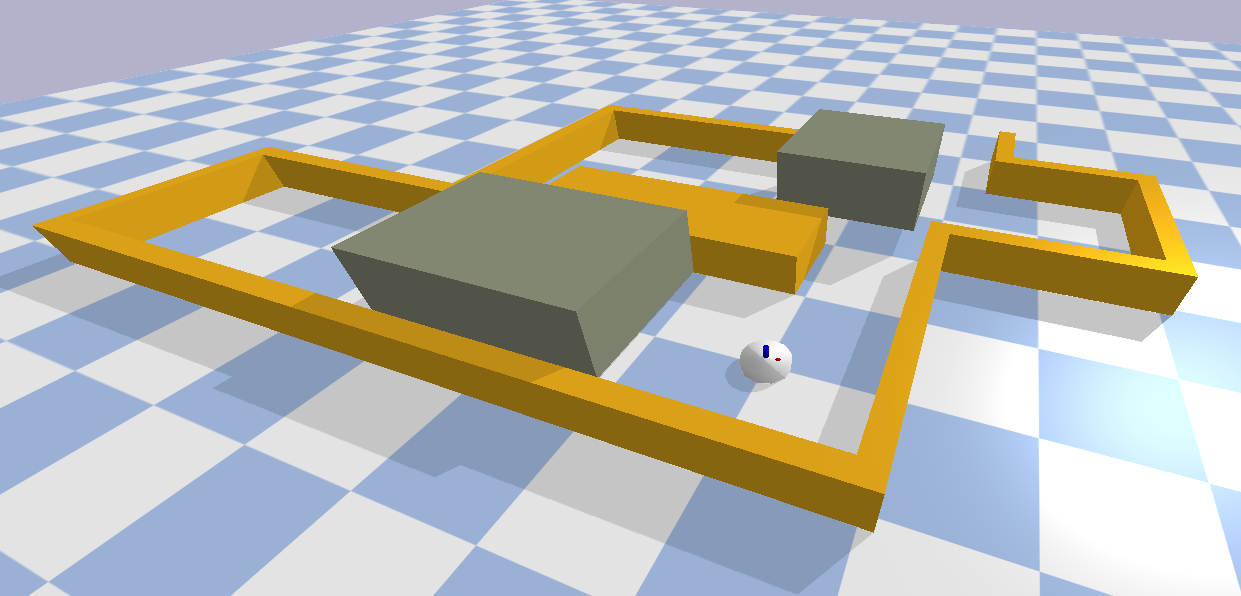
\includegraphics[width=0.8\textwidth]{figures/planning/two_push_to_freedom_env}
    \caption{Environment with the pointrobot, unmovable yellow walls and movable brown boxes.}%
    \label{fig:two_pushes_to_freedom_env}
\end{figure}

The point robot has an cylinderical shape thus a 2 dimensional configuration space is created and can be seen in \cref{fig:two_pushes_to_freedom_conf_space}.

\begin{figure}[H]
  \centering
  \begin{subfigure}{.49\textwidth}
    \centering
    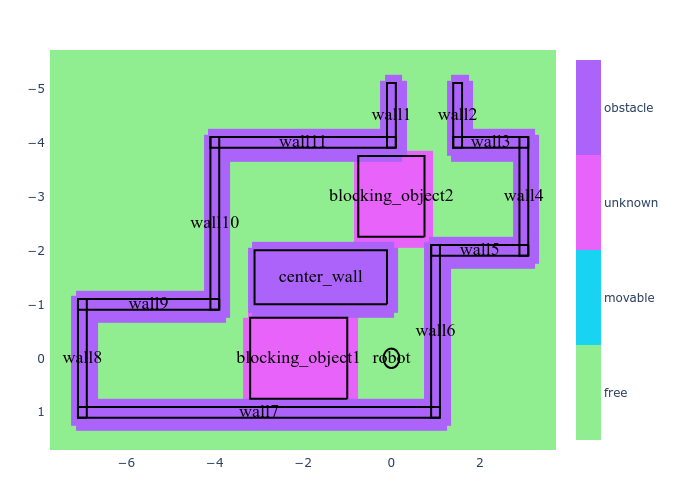
\includegraphics[width=1.05\textwidth]{figures/planning/c_space_point_robot_grid_size_0_1}
    \caption{$\gls{cspace}^{circle}$ with $\gls{cellSize} = 0.1$}%
    \label{fig:c_space_two_pushes_small}
  \end{subfigure}
  \begin{subfigure}{.49\textwidth}
    \centering
    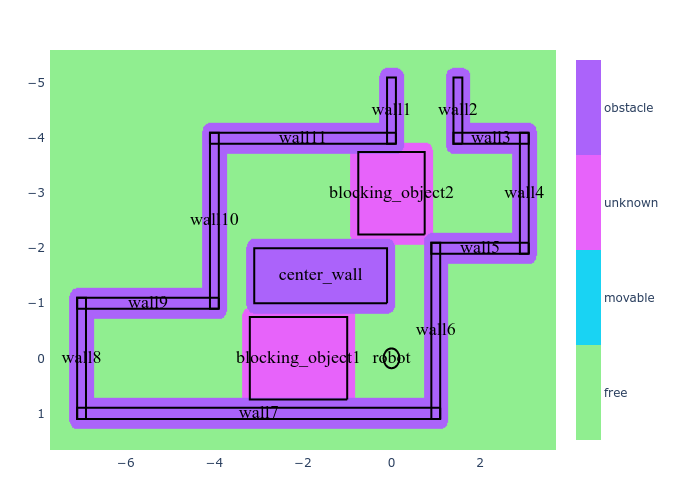
\includegraphics[width=1.05\textwidth]{figures/planning/c_space_point_robot_grid_size_0_01}
    \caption{$\gls{cspace}^{circle}$ with $\gls{cellSize} = 0.01$}%
    \label{fig:c_space_two_pushes_smaller}
  \end{subfigure}
  \caption{The configuration space for the point robot with different cell sizes. The robot\\environment corresponds to the environment presented in \cref{fig:two_pushes_to_freedom_env}.}
  \label{fig:two_pushes_to_freedom_conf_space}
\end{figure}

The resolution of the configuration space at \cref{fig:c_space_two_pushes_smaller} is higher compared to \cref{fig:c_space_two_pushes_small} because of the smaller grid size. The difference in resolution is especially visable at the corners of the walls. A high resolution is better at detecting paths through small quoridors and tight corners, but it comes at the cost of a longer creation and search time.

\paragraph{Path Existence Algorithm}
In context of this thesis we can describe path existence as: \textit{For an object's configuration space there exist an list of neighboring cells from starting to target configuration that do not lie in obstacle space.\bs}

A path in configuration space is detected using the implemented $f_\mathit{shortest\_path}(\gls{c}_\mathit{start}, \gls{c}_\mathit{target}, detect\_blocking\_objects)$ function. This function returns a shortest path from the $\gls{c}_\mathit{start}$ to the $\gls{c}_\mathit{target}$. \textit{detect\_blocking\_objects} is a boolean flag that if \textit{True} returns a list blocking objects that are classified as movable or unknown. If no path can be found, the $f_\textit{shortest\_path}$ function raises an error.\bs

The \textit{shortest\_path} function uses the Dijkstra algorithm 
\cite{dijkstra_note_1959} on the configuration space to find a shortest path. This path can be converted to provide a initial number of samples for motion or manipluation planners, also referreed to as a \quotes{warm start}.

\paragraph{Unfeasible solutions and an undecidable problem}
The path estimation algorithms does not take system constraints into account. It is thus possible that the path estimation algorithm finds a list of neighboring cells from the start to the target configuration and concludes that there exist a path. In reality, this path is unfeasible. An example is driving the boxer robot displayed in \cref{subfig:example_boxer_robot} through a narrow, sharp corner. Whilst geometrically the robot would fit through the corner, the nonholonomic constraints of the robot prevent it from steering through such a thight corner. It is for the motion or manipulation planner to detect that the path is unfeasible.\\

The path estimator suffers from another drawback, finding proof that there exists a path that is undecidable~\cite{zhang_simple_2008}. This is due to the chosen cell size during discretising the configuration space. An example is a quoridor that has exactly the width of the robot, the robot does fit exactly through this quoridor. Detecting such a path requires a number of neighboring cells that lie exactly in the centre line of the quoridor. Only with a cell size going to zero, and the number of cells going to infinity such a path is guaranteed to be detected. Path non-existence on the other hand is more easily to proof, since the path estimation algorithm provides a upper bound on existing paths and a lower bound on non-existing paths~\cite{zhang_simple_2008}.\bs

The path existence algorithm can detect non-existence paths. Thus checking path existence before motion or manipulation planning filters out a number of non-existent paths that would otherwise waste time and resources. Even if in exceptional cases the path estimation algorithm can yield unfeasible paths and can fail to detect existing paths. Checking path existence before motion or manipulation planning filters a number of non-exist paths and is additionally motivated by two reasons. First, because \cref{fig:speed_comparison_planning} shows that an path estimation is orders of magnitudes faster compared to motion or manipulation planning. Secondly, because the path estimation algorithm can provide a number of initial samples to the motion or manipulation planner that can act as a \quotes{warm start}.

\subsection{Motion Planning}%
\label{subsec:motion_planning}
Controllers discussed in \cref{sec:control_methods} can track a path from start to target. Providing a path is the motion planners' responsibility, motion planners seek inside the configuration space for a path from the start to the target configuration. A practical example of such a path is a list of successive robot poses, from starting pose (coinciding with the starting configuration) toward the target pose, where the successive poses lie close together 
\todo[inline]{smsmmsmssm 20 timesamplesThe }
(reachable for the robot in $\sim20$ time samples). Seeking a path from start to target inside a configuration space whilst avoiding obstacles for the robot to track is referred to as \textit{motion planning}. Finding a path between the start and target configuration for pushing applications whilst avoiding collisions is referred to as \textit{manipulation planning}. First, this subsection presents motion planning, and the next subsection \cref{subsec:manipulation_planning} dedicates itself to manipulation planning. For both motion and manipulation planning and sampling-based methods are used, which can be described as.\bs

\textit{\quotes{The main idea is to avoid the explicit construction of the object space, and instead conduct a search that probes the configuration space with a sampling scheme. This probing is enabled by a collision detection module, which the motion planning algorithm considers as a “black box.”~\cite{lavalle_planning_2006}}}\bs

Generally, the configuration space motion planners plan consists of 2 subspaces, free and obstacle space. The configuration space in this thesis consists of 4 subspaces, namely free, obstacle, unknown and movable space. To solve motion planning problems for such a configuration space a dedicated motion planning algorithm has been developed that extends the existing algorithm extends the existing double tree \ac{RRT*} algorithm~\cite{chen_fast_2018}. The motion planner consists of.
\begin{center}
\begin{tabular}[t]{l p{10cm}}
$V$:& A set of nodes\\
$E$:& A set of edges\\
$P$:& A set of paths\\
\end{tabular}
\end{center}

The start connectivity tree consists of the nodes connected by edges containing the starting node, and vice versa for the target connectivity tree containing the target node. The algorithm grows the two \textit{connectivity trees} by randomly sampling configurations and adding them to the start or target connectivity tree. The algorithm explores configuration space by growing these connectivity trees. When the start connectivity tree meets the target connectivity tree a path from start to target is found.\bs

Newly sampled configurations are added in a structural manner that guarantees an optimal path is found with infinite sampling. Where optimality is defined as the path with the lowest cost.

\todo[inline]{Corrado: This is also your idea right? If you put it like this it sounds like it’s common practice from the literature }

The cost is defined as a sum of a distance metric and a fixed penalty for paths that cross unknown or movable subspaces. Incentivising the algorithm to find a path around unknown or movable obstacles over a path crossing through unknown or movable obstacles.\bs

The algorithm takes in 2 arguments, first the \textit{step size}, the maximal normalised distance between connected samples in the connectivity trees. Second, the \textit{search size} is a subspace around newly sampled samples, inside this subspace a parent node is saught that results in the lowest cost, rewiring of closeby nodes happens and the other connectivity tree is searched to detect a full path from start to target.\bs

Now pseudocode of the proposed algorithm is provided in \cref{pseudocode:proposed_rrt_star}, and functions used are elaborated on in \cref{table:functions_for_proposed_rrt_star}. The coloured sections inside \cref{pseudocode:proposed_rrt_star} correspond to the surrounding coloured box around subfigures in \cref{fig:motion_planner_adding_one_sample}. The following definitions are used by the proposed algorithm.\bs

\todo[inline]{It is a suprise to suddenly read that there apparently is a "proposed algorithm". The chapter/section intro doesn't mention that something will be proposed, and neither does all of the text leading up to this sentence.}


\begin{table}[H]
\centering
\begin{tabular}[t]{l p{10cm}}
$x$:& A node containing a point in configuration space\\
$x_{init}$:& Creates a start and target node\\ 
$NotReachStop$:& True if the stopping criteria is not reached\\ 
$Sample_{random}$:& Creates a random sample in free-, movable- or unknown space\\
$Nearest(x, V)$:& Returns the nearest nodes from $x$ in $V$\\
$NearestSet(x, V)$:& Returns set of nearest nodes from $x$ in $V$\\
$Project(x, x')$:& Project $x$ toward $x'$\\
$CollisionCheck(x)$:& Returns true if $x$ is in free-, movable- or unknown space\\
$ObjectCost(x', x)$:& Returns a fixed additional cost if $x$ enters movable- or unknown space from $x'$, otherwise returns 0\\
$Distance(x, x')$:& Returns the distance between sample $x$ and $x'$\\
$CostToInit(x)$:& Find the total cost from $x$ to the initial node\\
$LocalPlannerCheck(x, x')$:& Return true if a local planner is able to connect $x$ and $x'$, otherwise return false. A system model (see \cref{sec:sys_iden}) acts a local planner\\
$InSameTree(x, x')$:& Returns true if both $x$ and $x'$ are in the same tree, otherwise return false\\
\end{tabular}
\caption{Functions used by the \cref{pseudocode:proposed_rrt_star}}
\label{table:functions_for_proposed_rrt_star}
\end{table}

\todo[inline]{you did not yet say anithing about modified RRT, stop that}
\newpage
\begin{algorithm}[H]
\caption{Pseudocode for modified $\text{RRT}^*$ algorithm taking movable objects and constraints into account}
\label{pseudocode:proposed_rrt_star}
\begin{algorithmic}[1]

\hspace{-0.9cm}\colorbox{my_grey}{\parbox{\linewidth}{%
\State $V \leftarrow x_{init}$
\While{$NotReachStop$} 

\hspace{-0.1cm}\colorbox{my_light_blue}{\parbox{\linewidth}{%
    \State $Cost_{min} \leftarrow +\infty$ \algorithmiccomment{Create, check and project a new random sample}
    \State $x_{rand} \leftarrow Sample_{random}$
    \State $x_{nearest} \leftarrow Nearest(x_{rand}, V)$
    \State $x_{temp} \leftarrow Project(x_{rand}, x_{nearest})$

    \If{$CollisionCheck(x_{temp})$}
        \State $x_{new} = x_{temp}$
        \Else
        \State $Continue$
    \EndIf
}}

\hspace{-0.1cm}\colorbox{my_yellow}{\parbox{\linewidth}{%
    \State $X_{near} \leftarrow NearestSet(x_{new}, V)$ \algorithmiccomment{Find and connect new node to parent node}
    \For{$x_{near} \in X_{near}$}
    \State $Cost_{temp} \leftarrow CostFromInit(x_{near}) + Distance(x_{near}, x_{new}) + ObjectCost(x_{near}, x_{new})$
    \If{$Cost_{temp}  < Cost_{min}$}
            \If{$LocalPlannerCheck(x_{new}, x_{near})$}
            \State $Cost_{min} \leftarrow x_{temp}$
            \State $x_{minCost} \leftarrow x_{near}$
            \EndIf
        \EndIf
    \EndFor
    \If{$Cost_{min} == \infty$}
        \State $Continue$
    \Else
        \State $V.add(x_{new})$
        \State $E.add(x_{minCost}, x_{new})$
    \EndIf
}}

\hspace{-0.1cm}\colorbox{my_green}{\parbox{\linewidth}{%
    \State $Cost_{path} \leftarrow +\infty$ \algorithmiccomment{Check if the newly added node can lower cost for nearby nodes}
    \For{$x_{near} \in X_{near}$} 
      \If{$InSameTree(x_{near}, x_{new})$} 
        \State $Cost_{temp} \leftarrow CostFromInit(x_{new}) + distance(x_{new}, x_{near}) + ObjectCost(x_{new}, x_{near})$
        \If{$Cost_{temp} < CostFromInit(x_{near})$}
           \If{$LocalPlannerCheck(x_{new}, x_{near})$}
              \State $E.rewire(x_{near}, x_{new})$
           \EndIf
        \EndIf
      \Else \algorithmiccomment{Add lowest cost path to list of paths}
          \State $Cost_{temp} \leftarrow CostFromInit(x_{new}) + distance(x_{new}, x_{near}) $ \newline\hspace*{10em} $+ CostFromInit(x_{near}) + ObjectCost(x_{new}, x_{near})$
          \If{$Cost_{temp}  < Cost_{path}$}
              \If{$LocalPlannerCheck(x_{new}, x_{near})$}
                  \State $Cost_{pathMin} \leftarrow x_{temp}$
                  \State $x_{pathMin} \leftarrow x_{near}$
              \EndIf
          \EndIf
      \EndIf
      \If{$Cost_{pathMin} == \infty$}
          \State $Continue$
      \Else
          \State $P.addPath(x_{new}, x_{pathMin}, Cost_{pathMin})$
      \EndIf
    \EndFor
}}

\EndWhile
}}
\end{algorithmic}
\end{algorithm}

\newpage
Now an example is provided of the proposed algorithm that creates and adds one sample in \cref{fig:motion_planner_adding_one_sample}. After adding the newly sampled sample is added to the start connectivity tree, a sample is rewired then the target connectivity tree is connected to the start connectivity tree. The resulting path found can be visualised in \cref{fig:motion_planner_comparison}.\bs

\begin{figure}[H]
    \centering
    \begin{subfigure}{.49\textwidth}
    \centering
    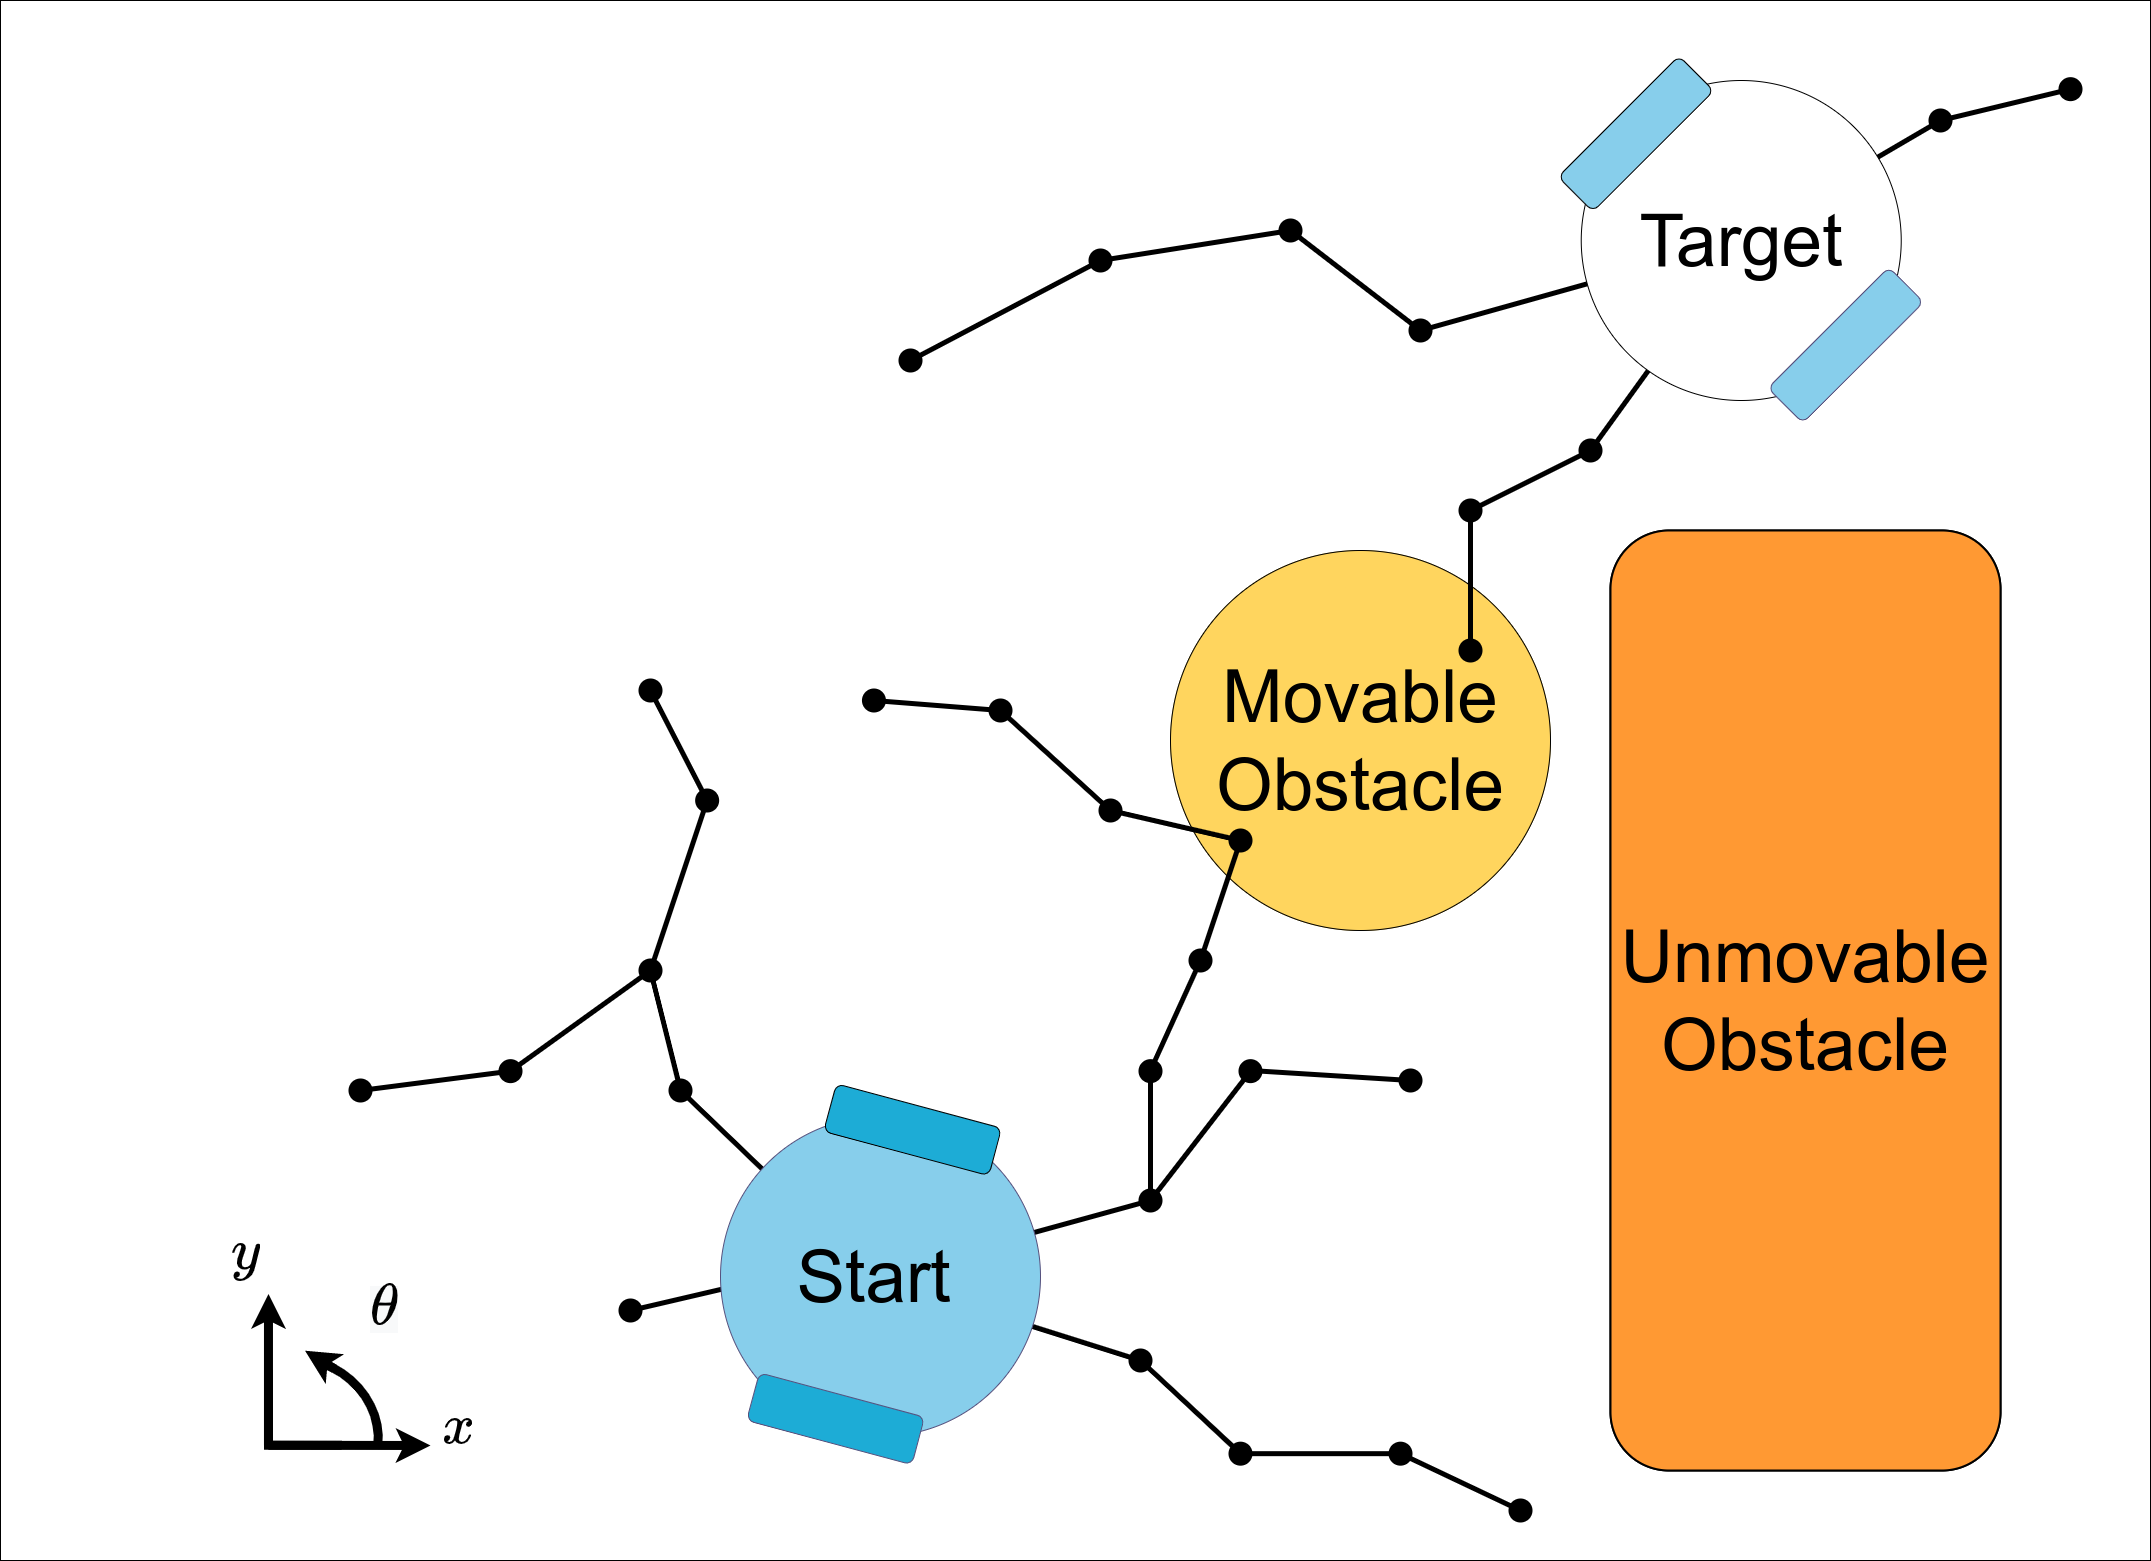
\includegraphics[width=0.93\textwidth, cfbox=my_grey 5pt 0pt]{figures/mp/1mp_init.drawio.png}
    \caption{Snapshot of the configuration space during a search\\from start to the target configuration.}
    \end{subfigure}
    \begin{subfigure}{.49\textwidth}
    \centering
    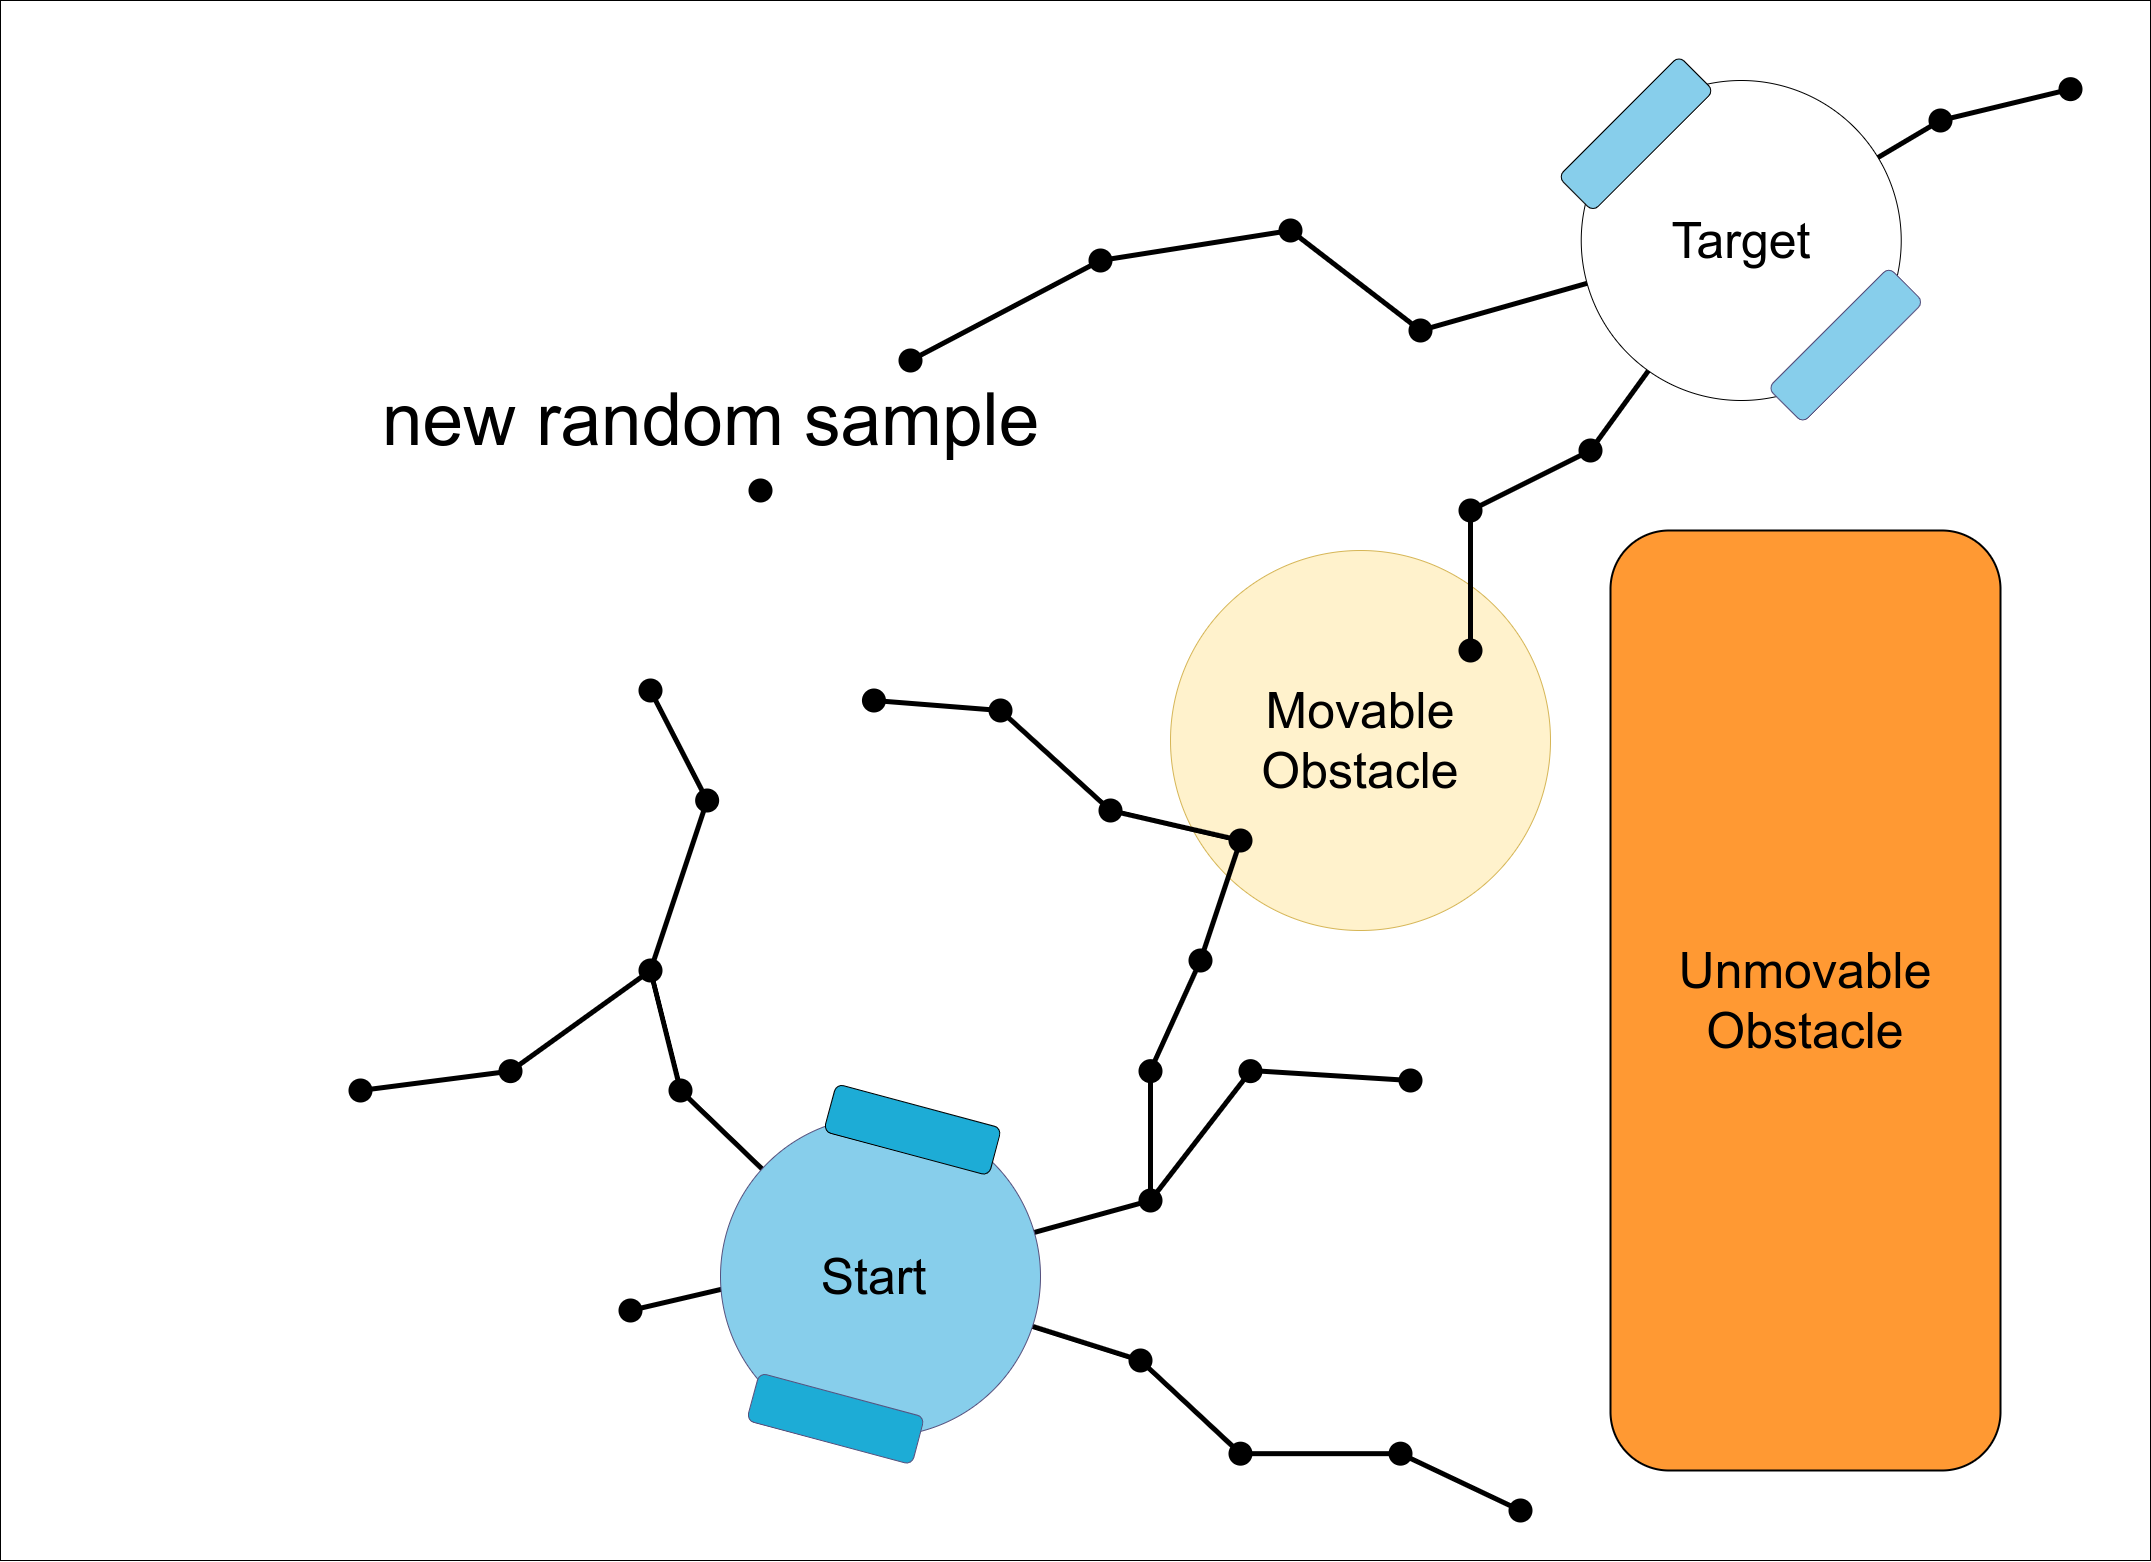
\includegraphics[width=0.93\textwidth, cfbox=my_light_blue 5pt 0pt]{figures/mp/2mp_new_rand_sample.drawio.png}
    \caption{A new random sample is generated.\bs}
    \end{subfigure}

    \begin{subfigure}{.49\textwidth}
    \centering
    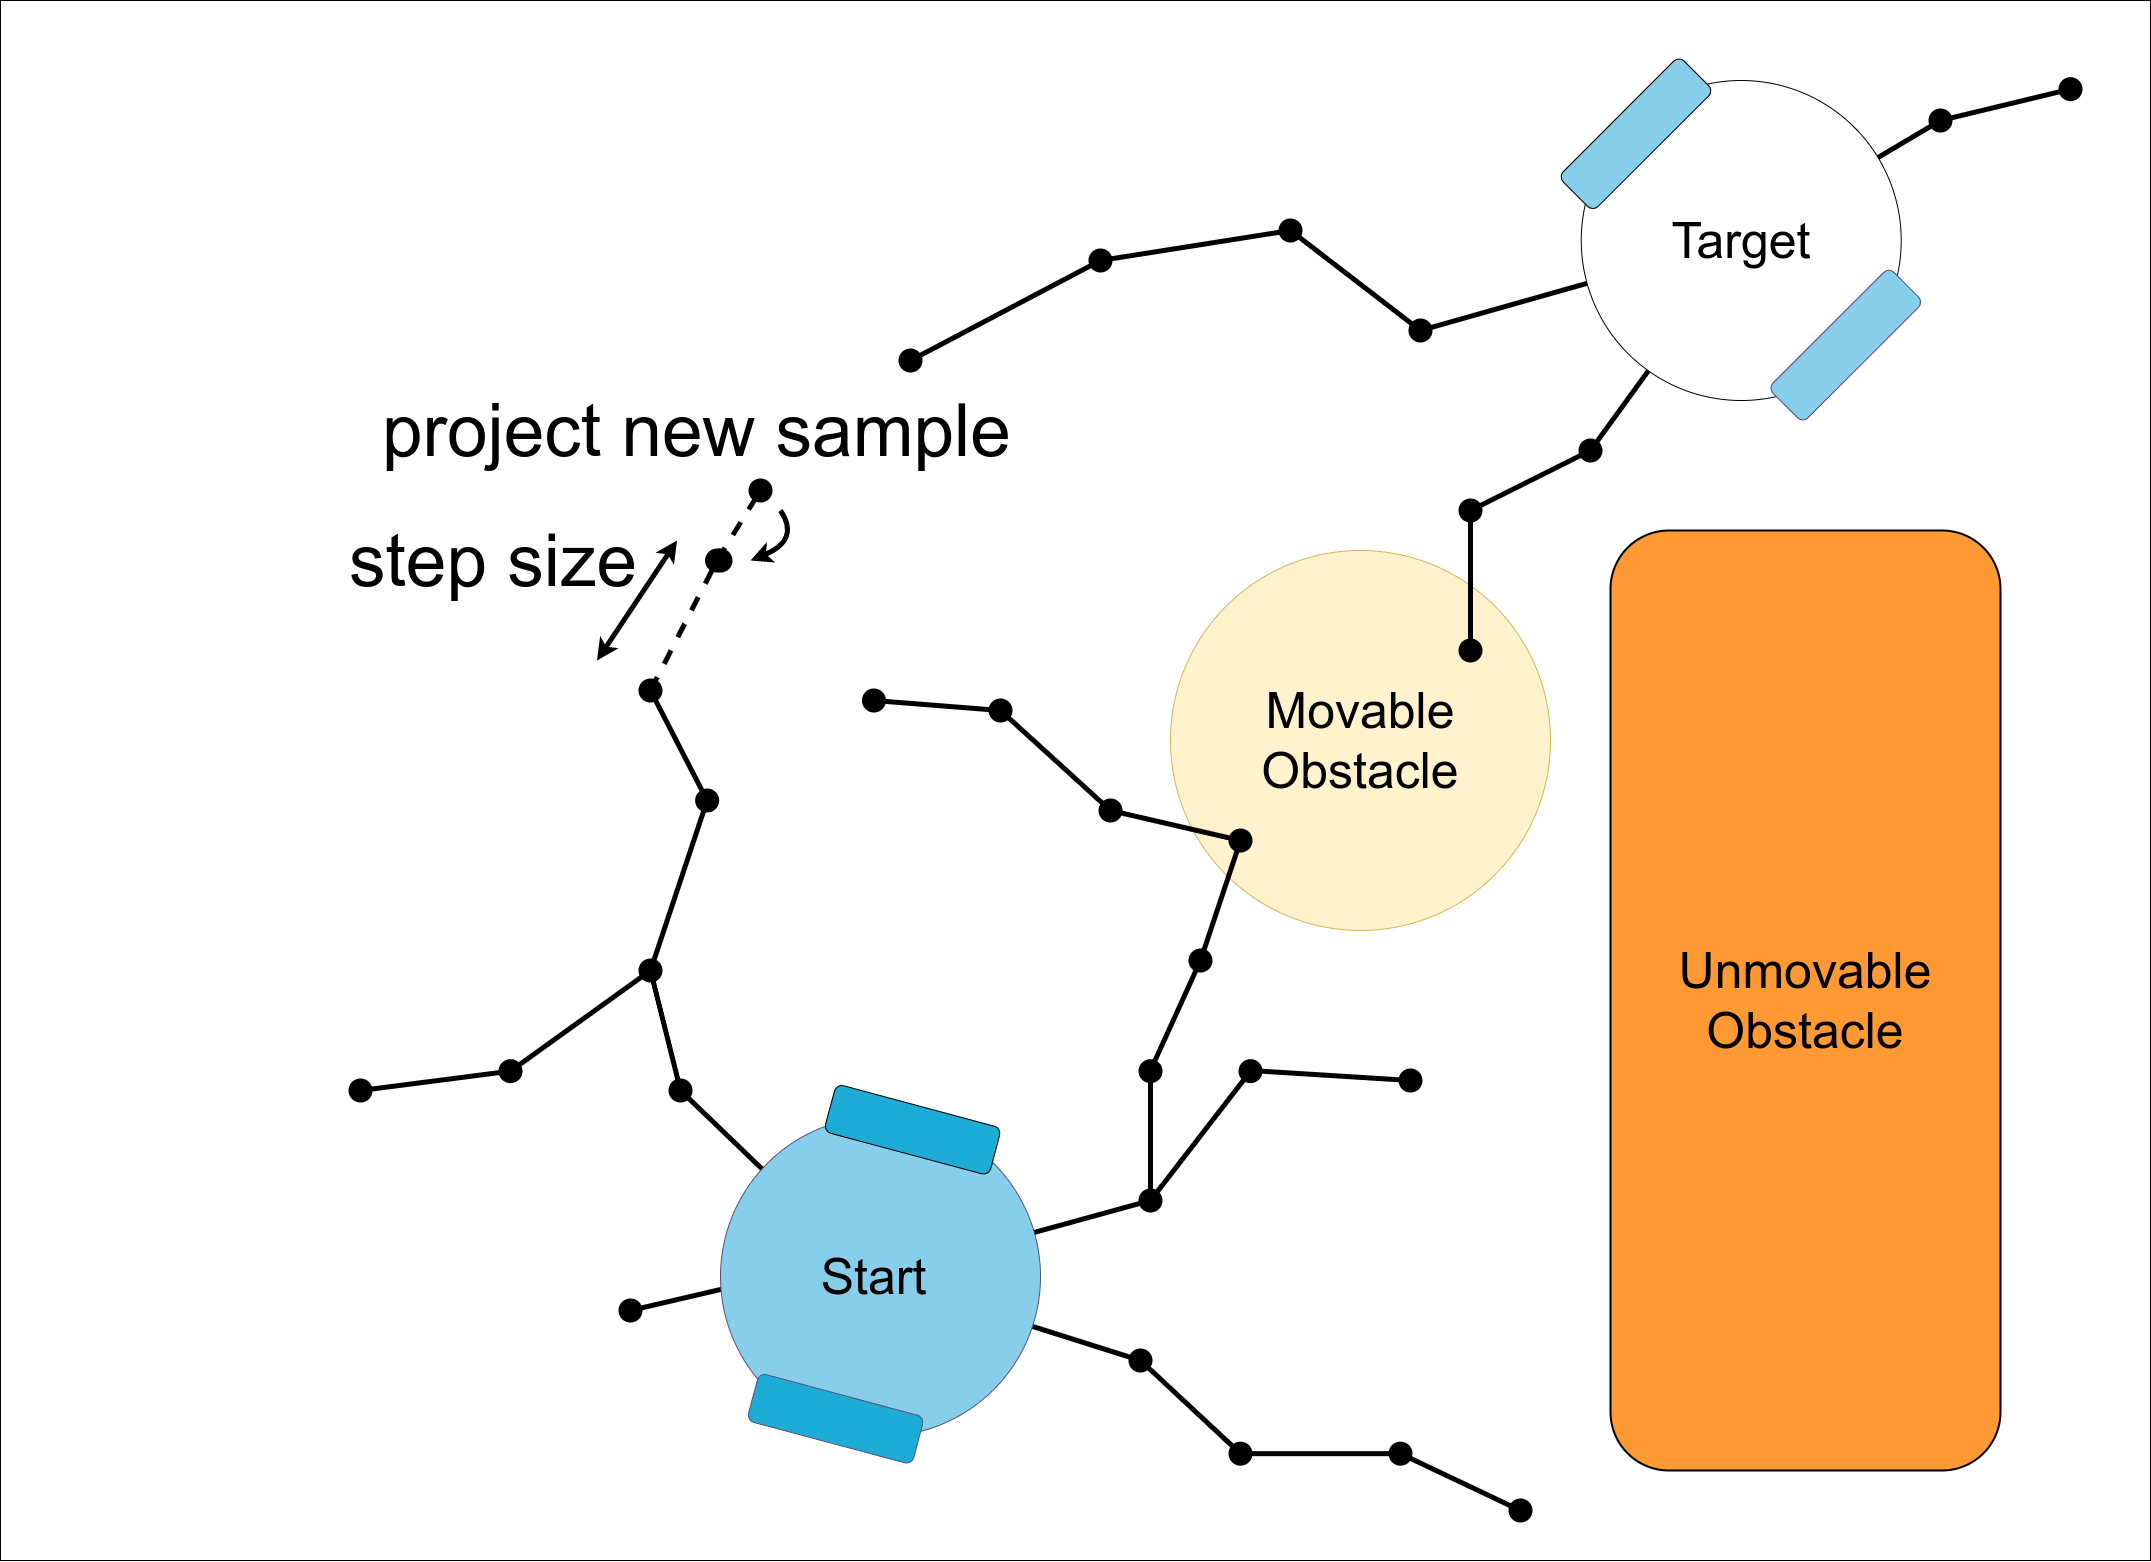
\includegraphics[width=0.93\textwidth, cfbox=my_light_blue 5pt 0pt]{figures/mp/3mp_project_sample.drawio.png}
    \caption{The new sample is projected toward the closest sample.\bs}
    \end{subfigure}
    \begin{subfigure}{.49\textwidth}
    \centering
    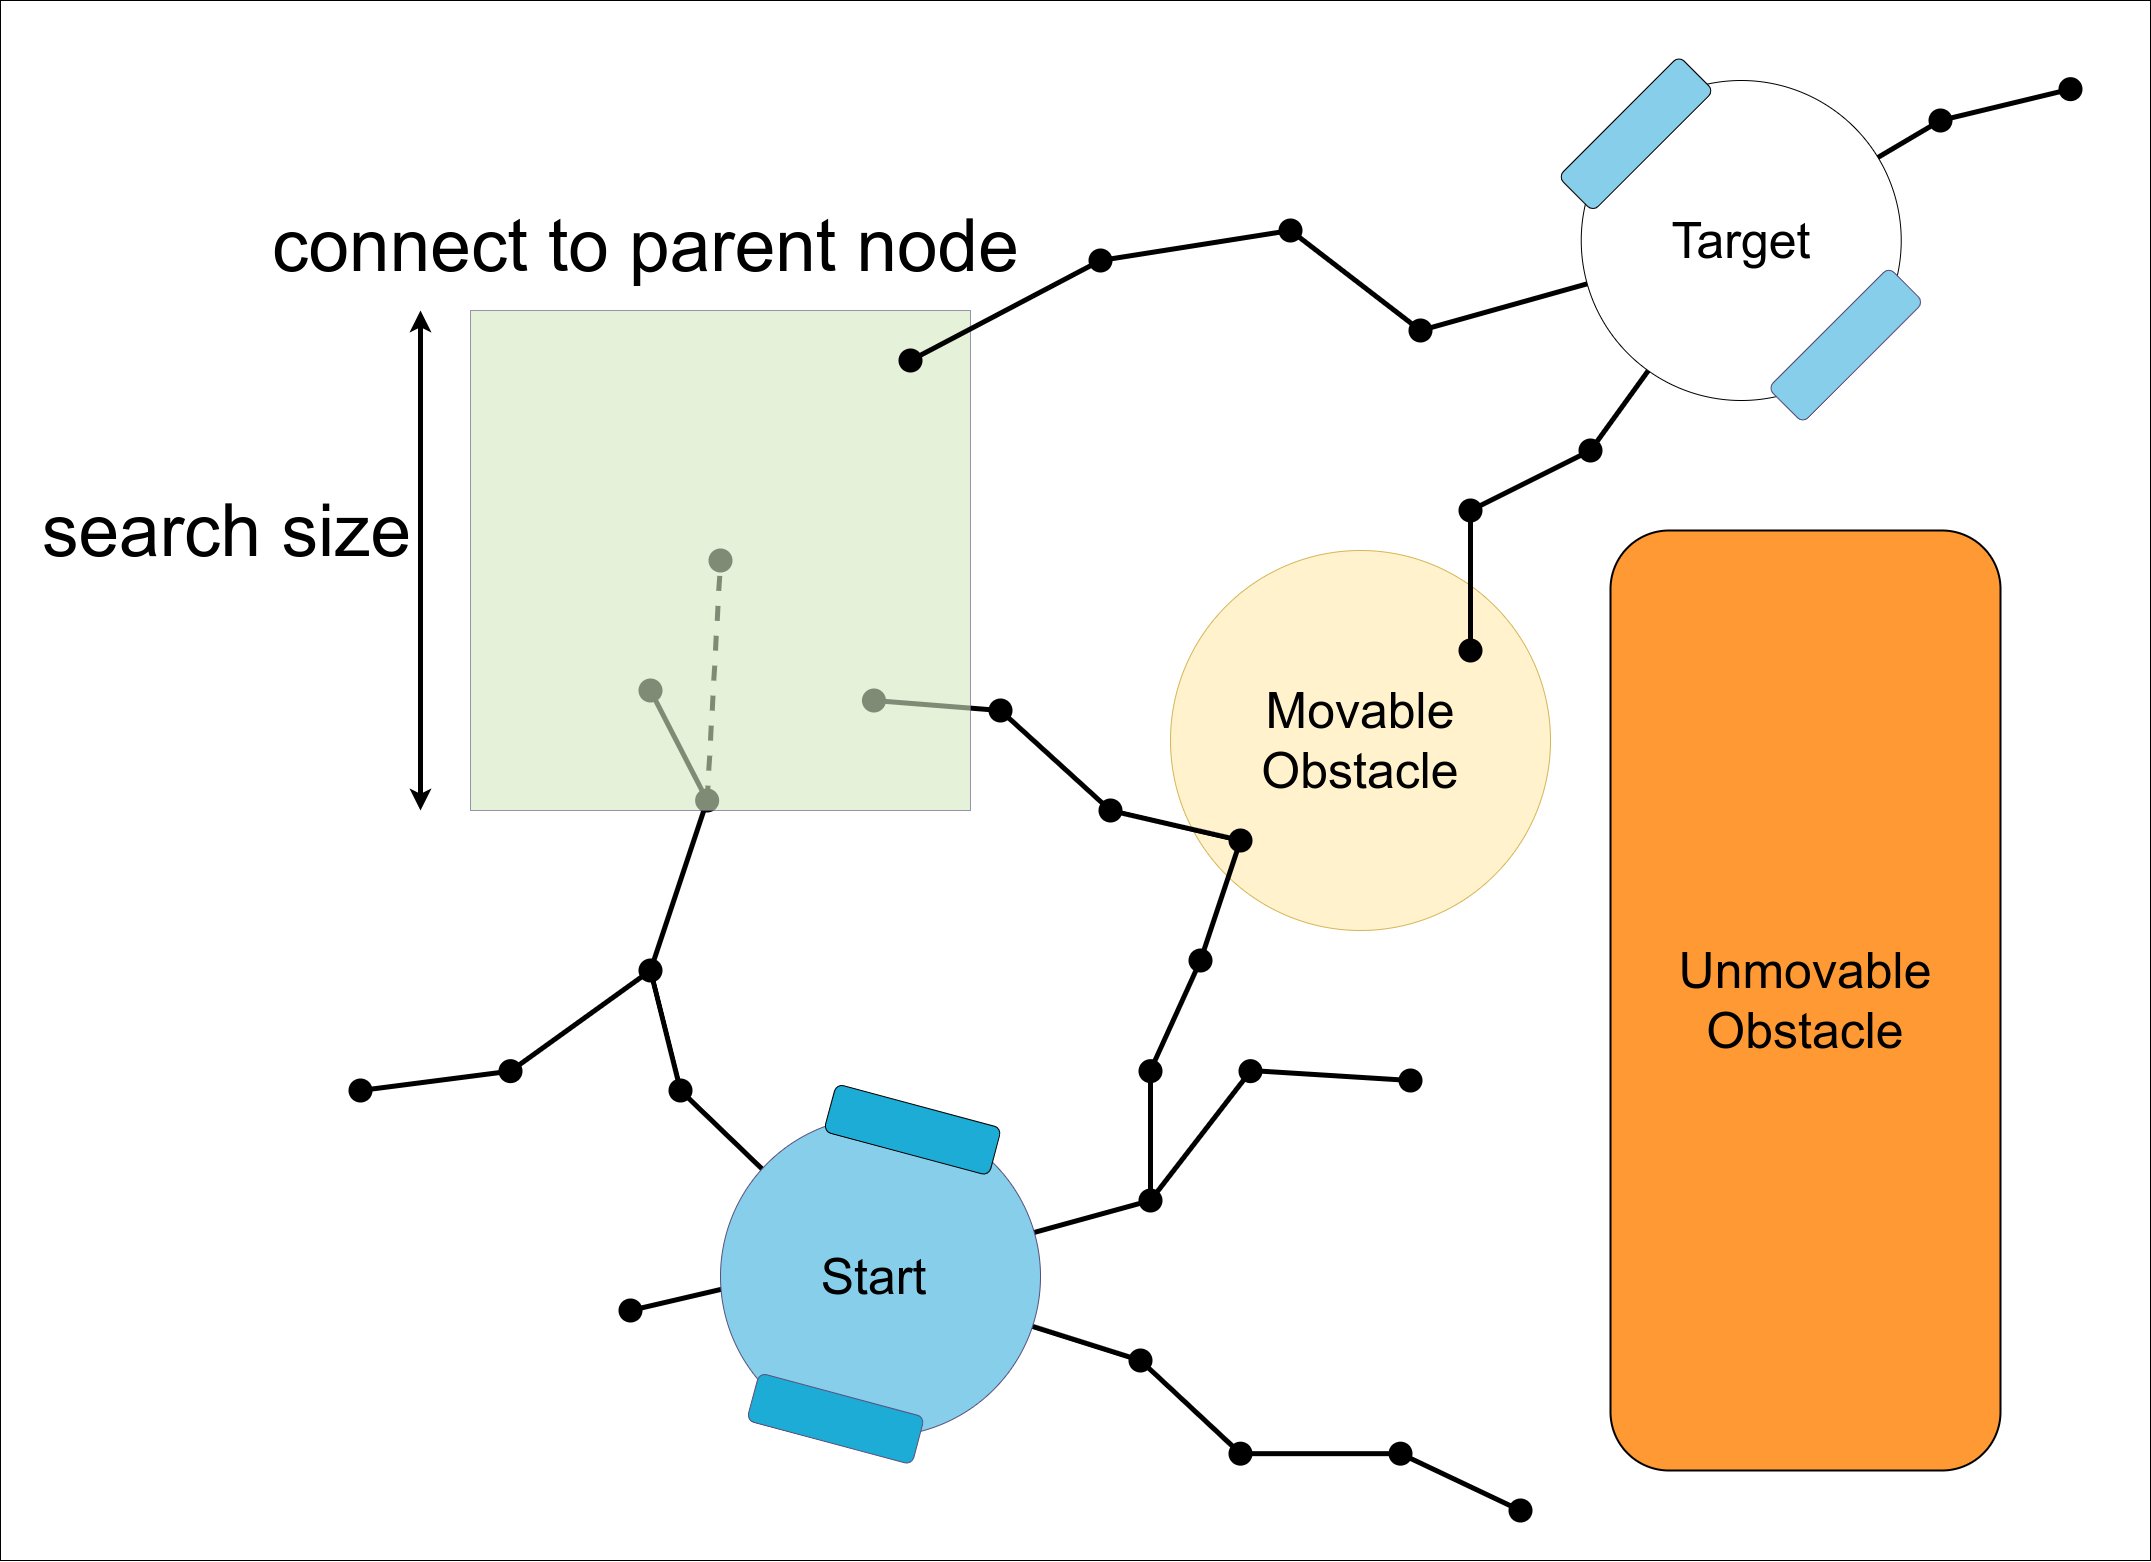
\includegraphics[width=0.93\textwidth, cfbox=my_yellow 5pt 0pt]{figures/mp/4mp_connect_to_tree.drawio.png}
    \caption{The new sample is connected to the node in search space\\that results in the lowest cost.}
    \end{subfigure}

    \begin{subfigure}{.49\textwidth}
    \centering
    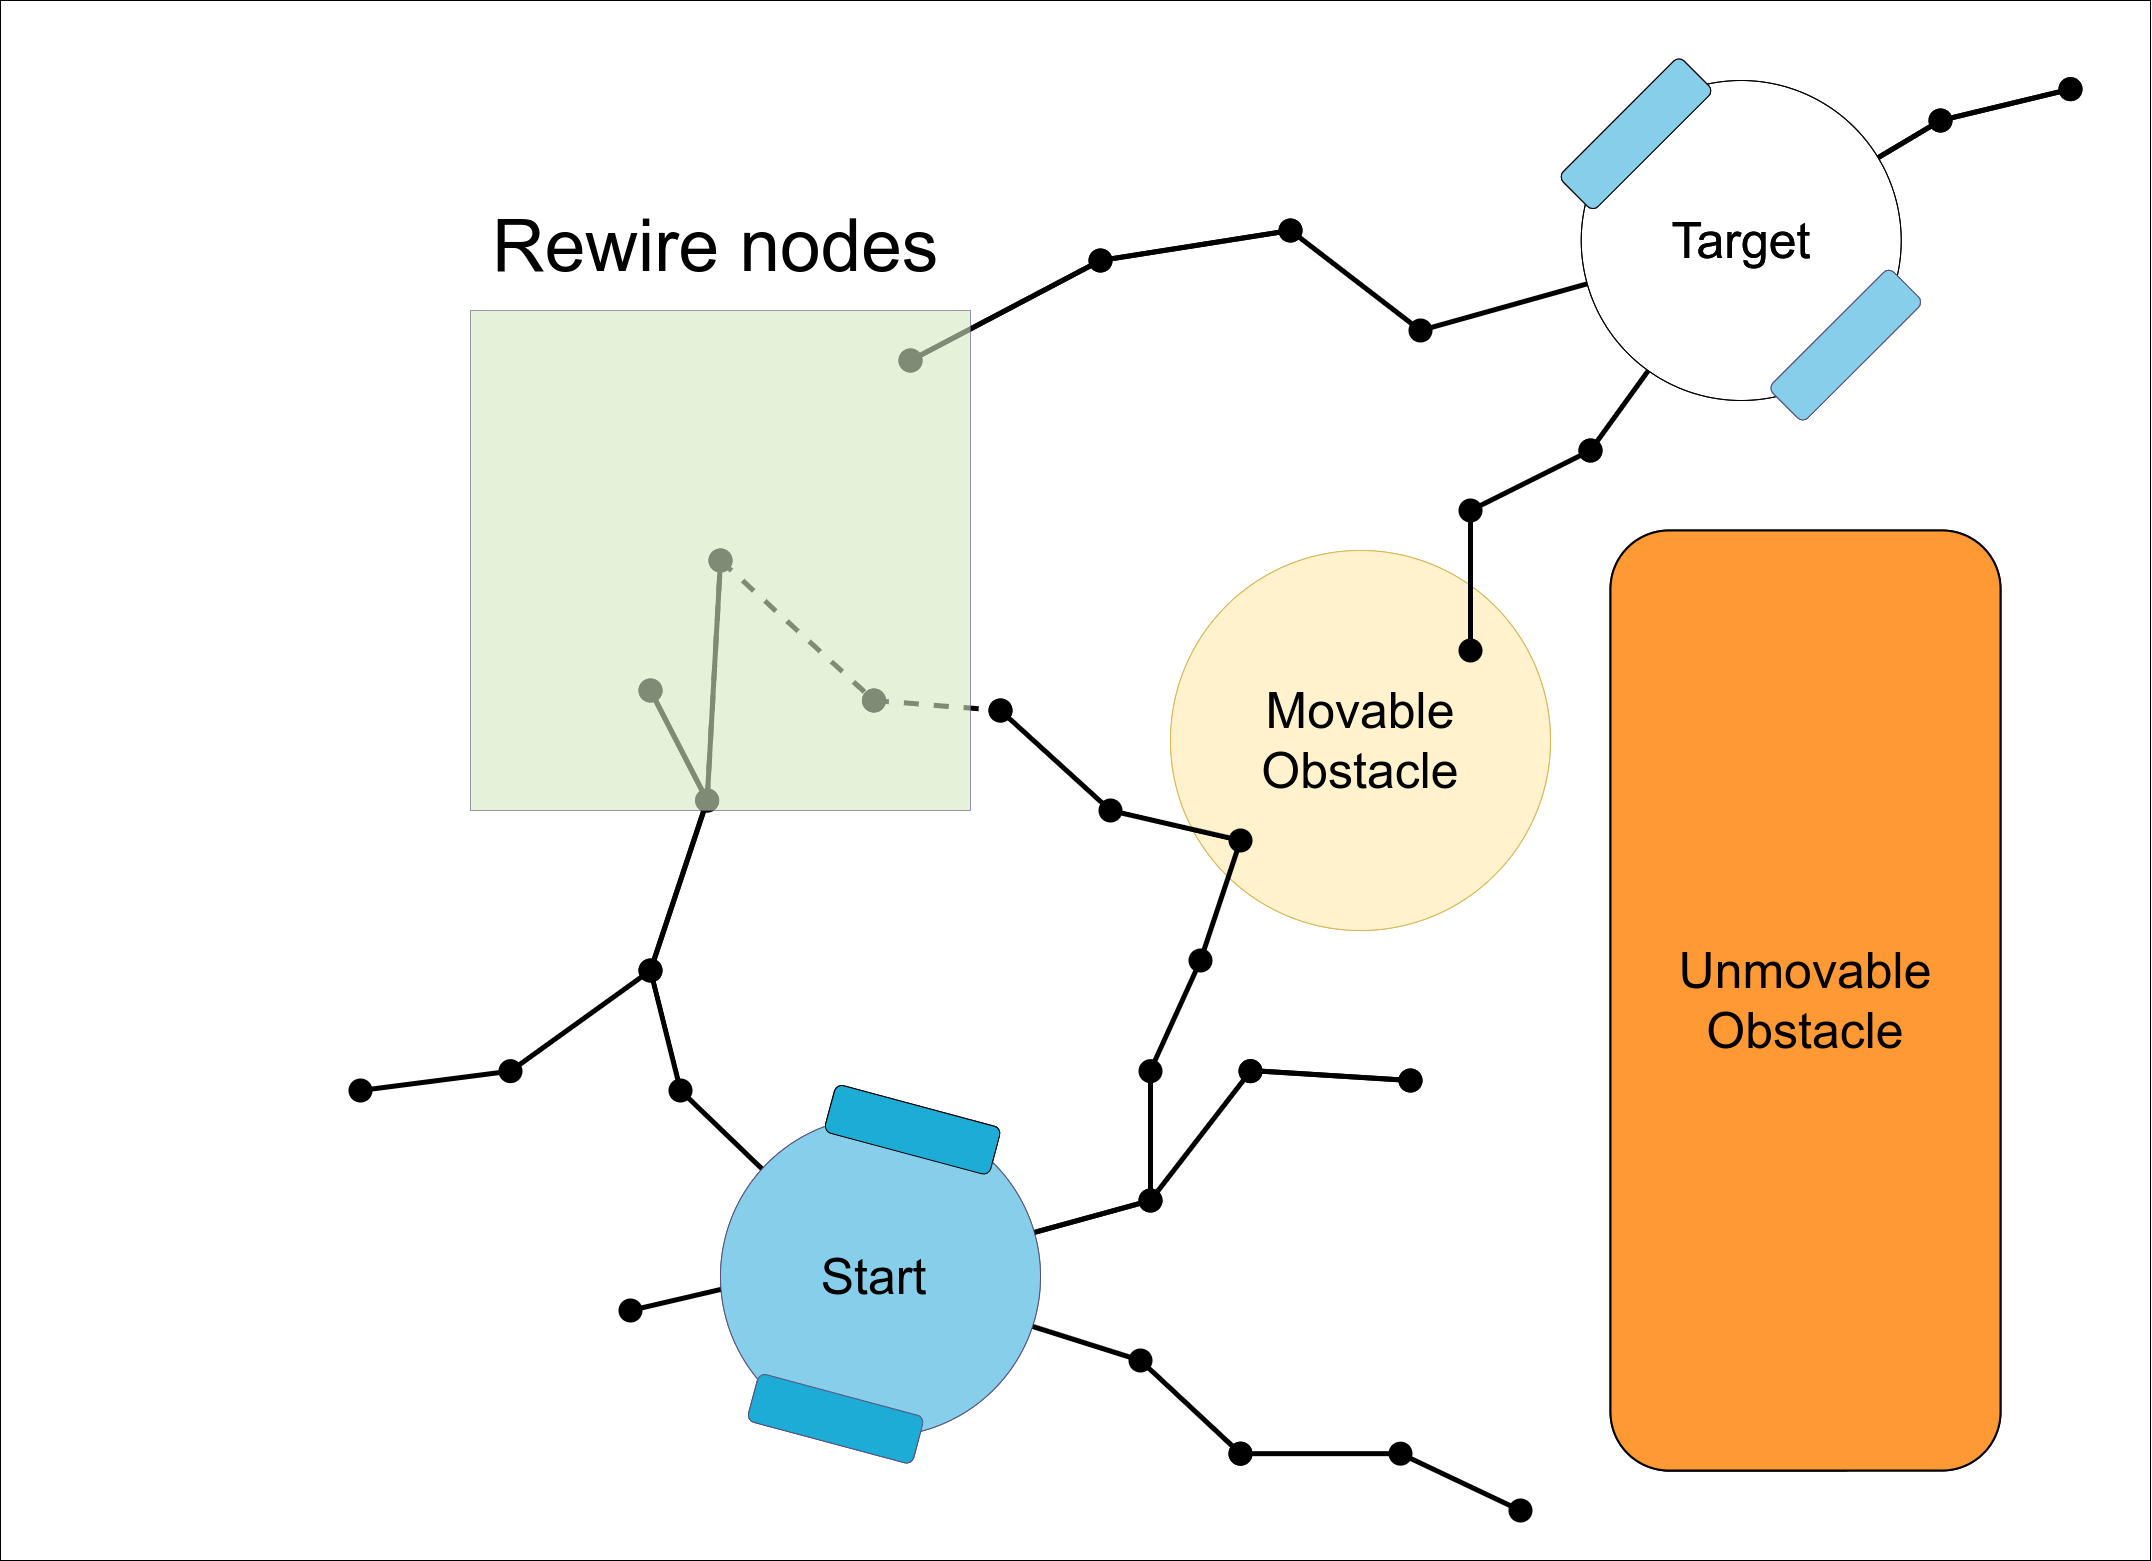
\includegraphics[width=0.93\textwidth, cfbox=my_green 5pt 0pt]{figures/mp/5mp_rewire.drawio.png}
    \caption{Nodes for which the cost can be lowered\\from the new sample are rewired.}
    \end{subfigure}
    \begin{subfigure}{.49\textwidth}
    \centering
    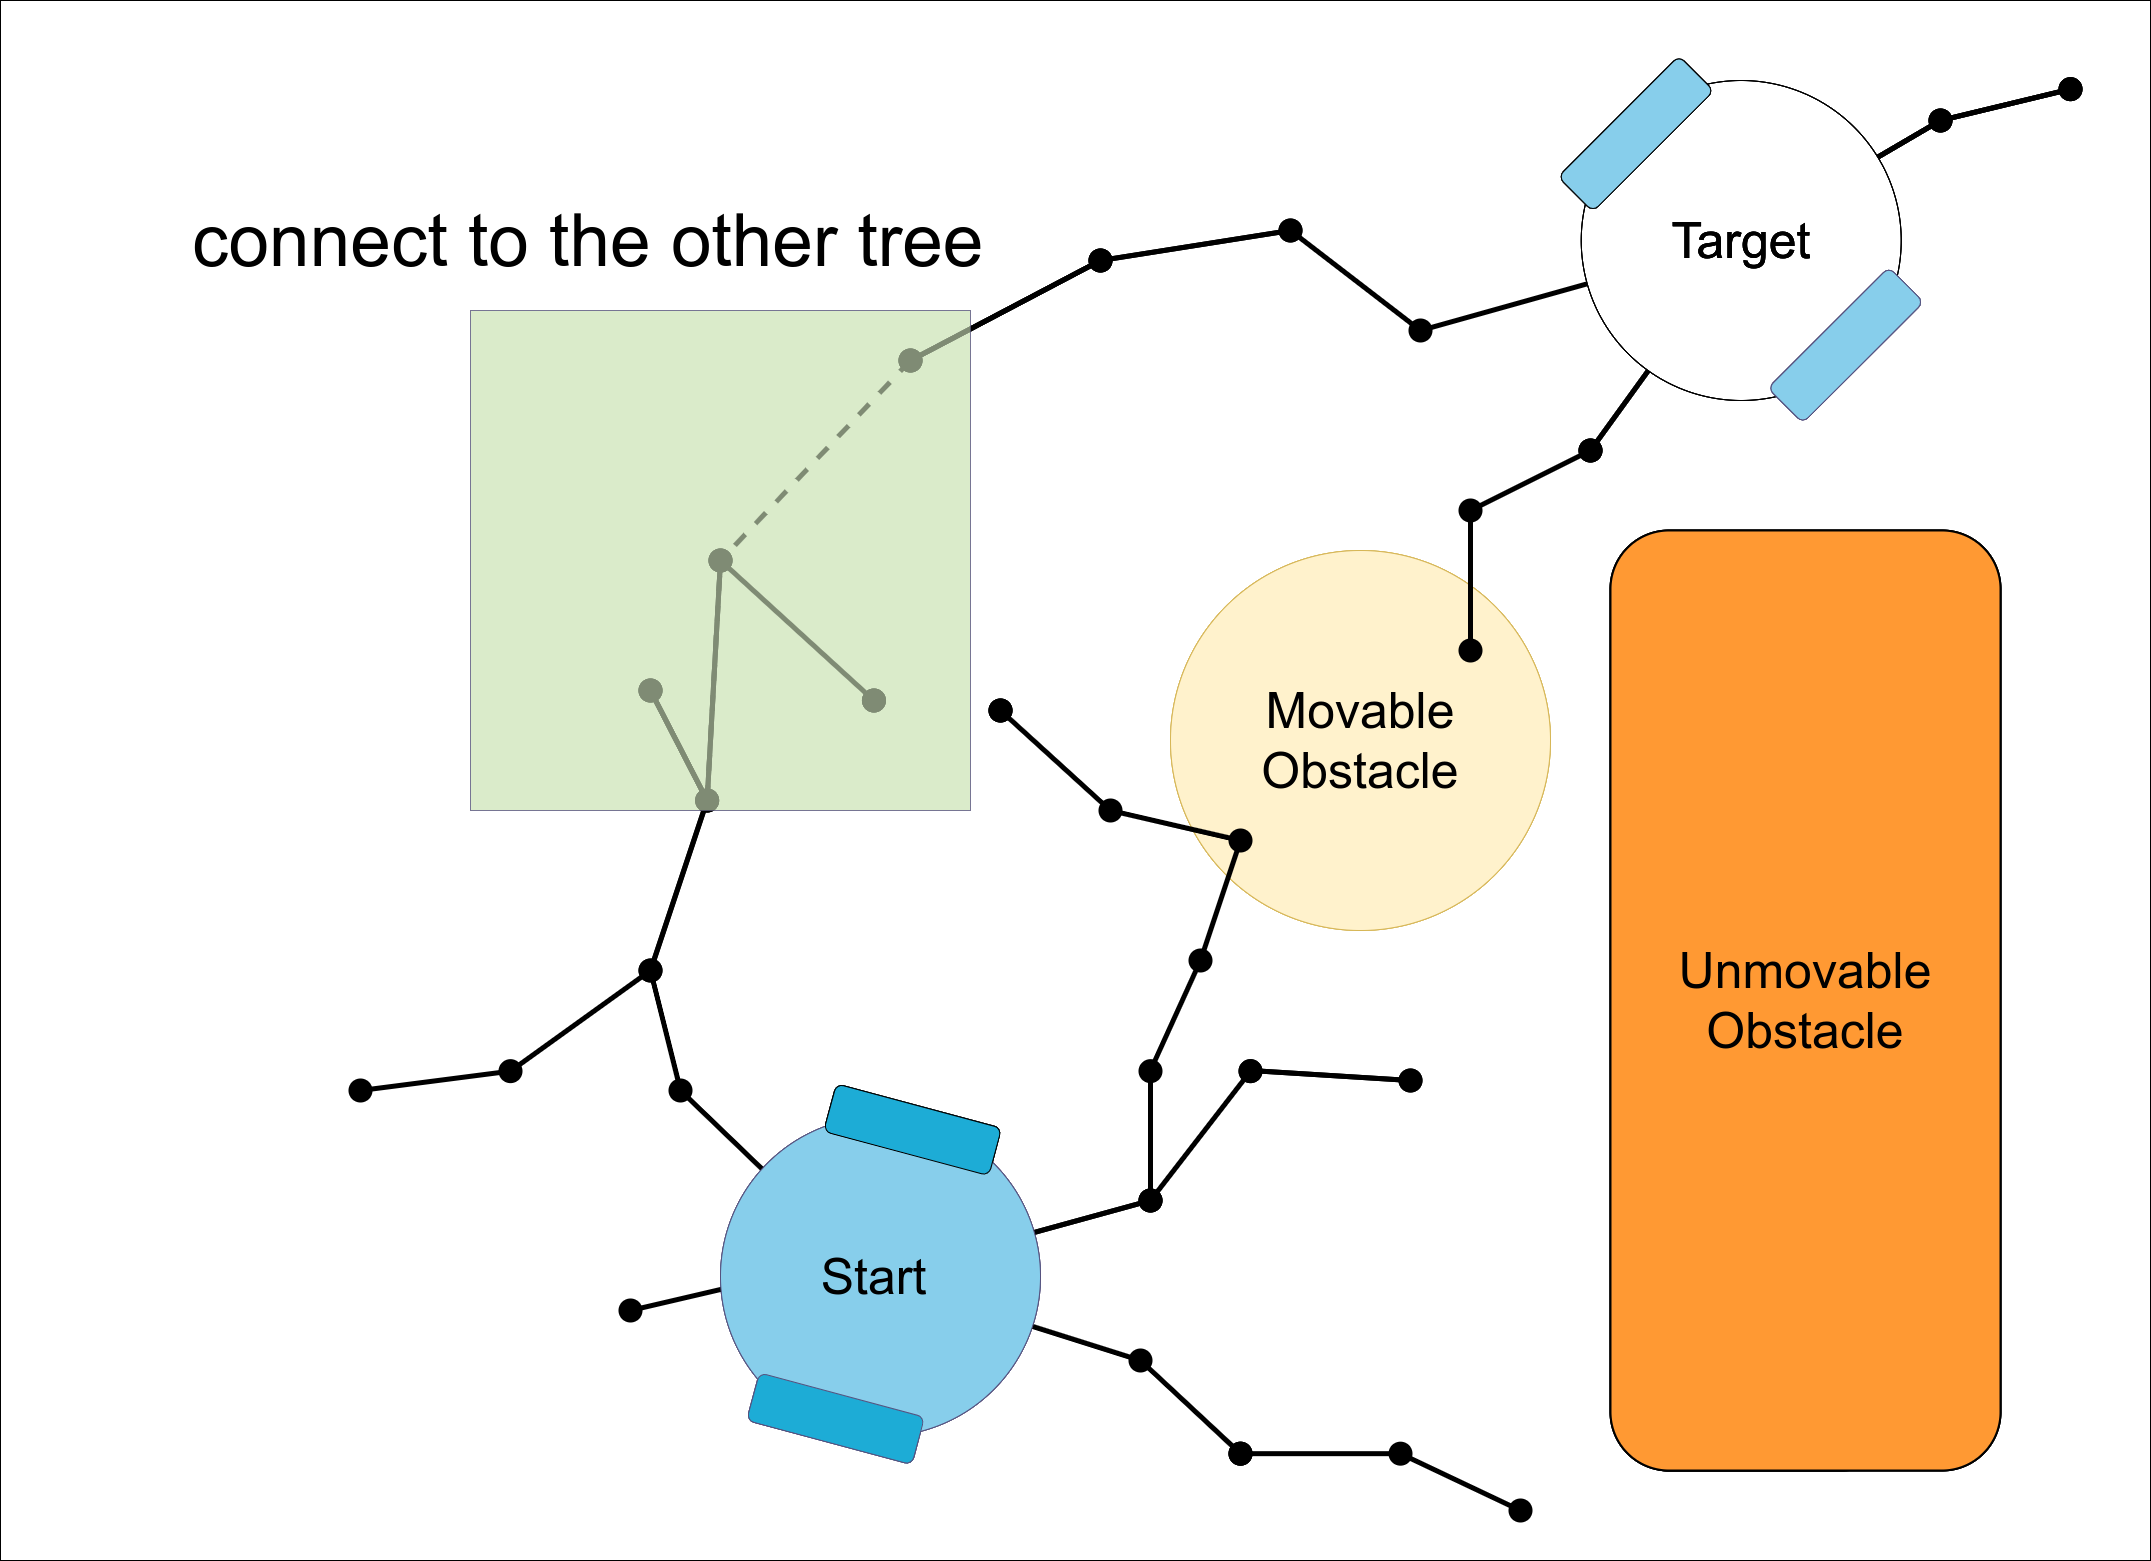
\includegraphics[width=0.93\textwidth, cfbox=my_green 5pt 0pt]{figures/mp/6mp_search_other_tree.drawio.png}
    \caption{A path from start to target configuration is found. \bs}
    \end{subfigure}

    \caption{Visualisation of the Double tree \acs{RRT*} motion planner that adds a single sample to the connectivity graph. The colour of the box surrounding subfigures corresponds to the coloured sections in \cref{pseudocode:proposed_rrt_star}. 3-dimensional configuration space displayed as 2-dimensional configuration space ($x$ and $y$ are visible, $\theta$ is not visible).}
    \label{fig:motion_planner_adding_one_sample}
\end{figure}


\begin{figure}[H]
    \centering
    \begin{subfigure}{.5\textwidth}
    \centering
    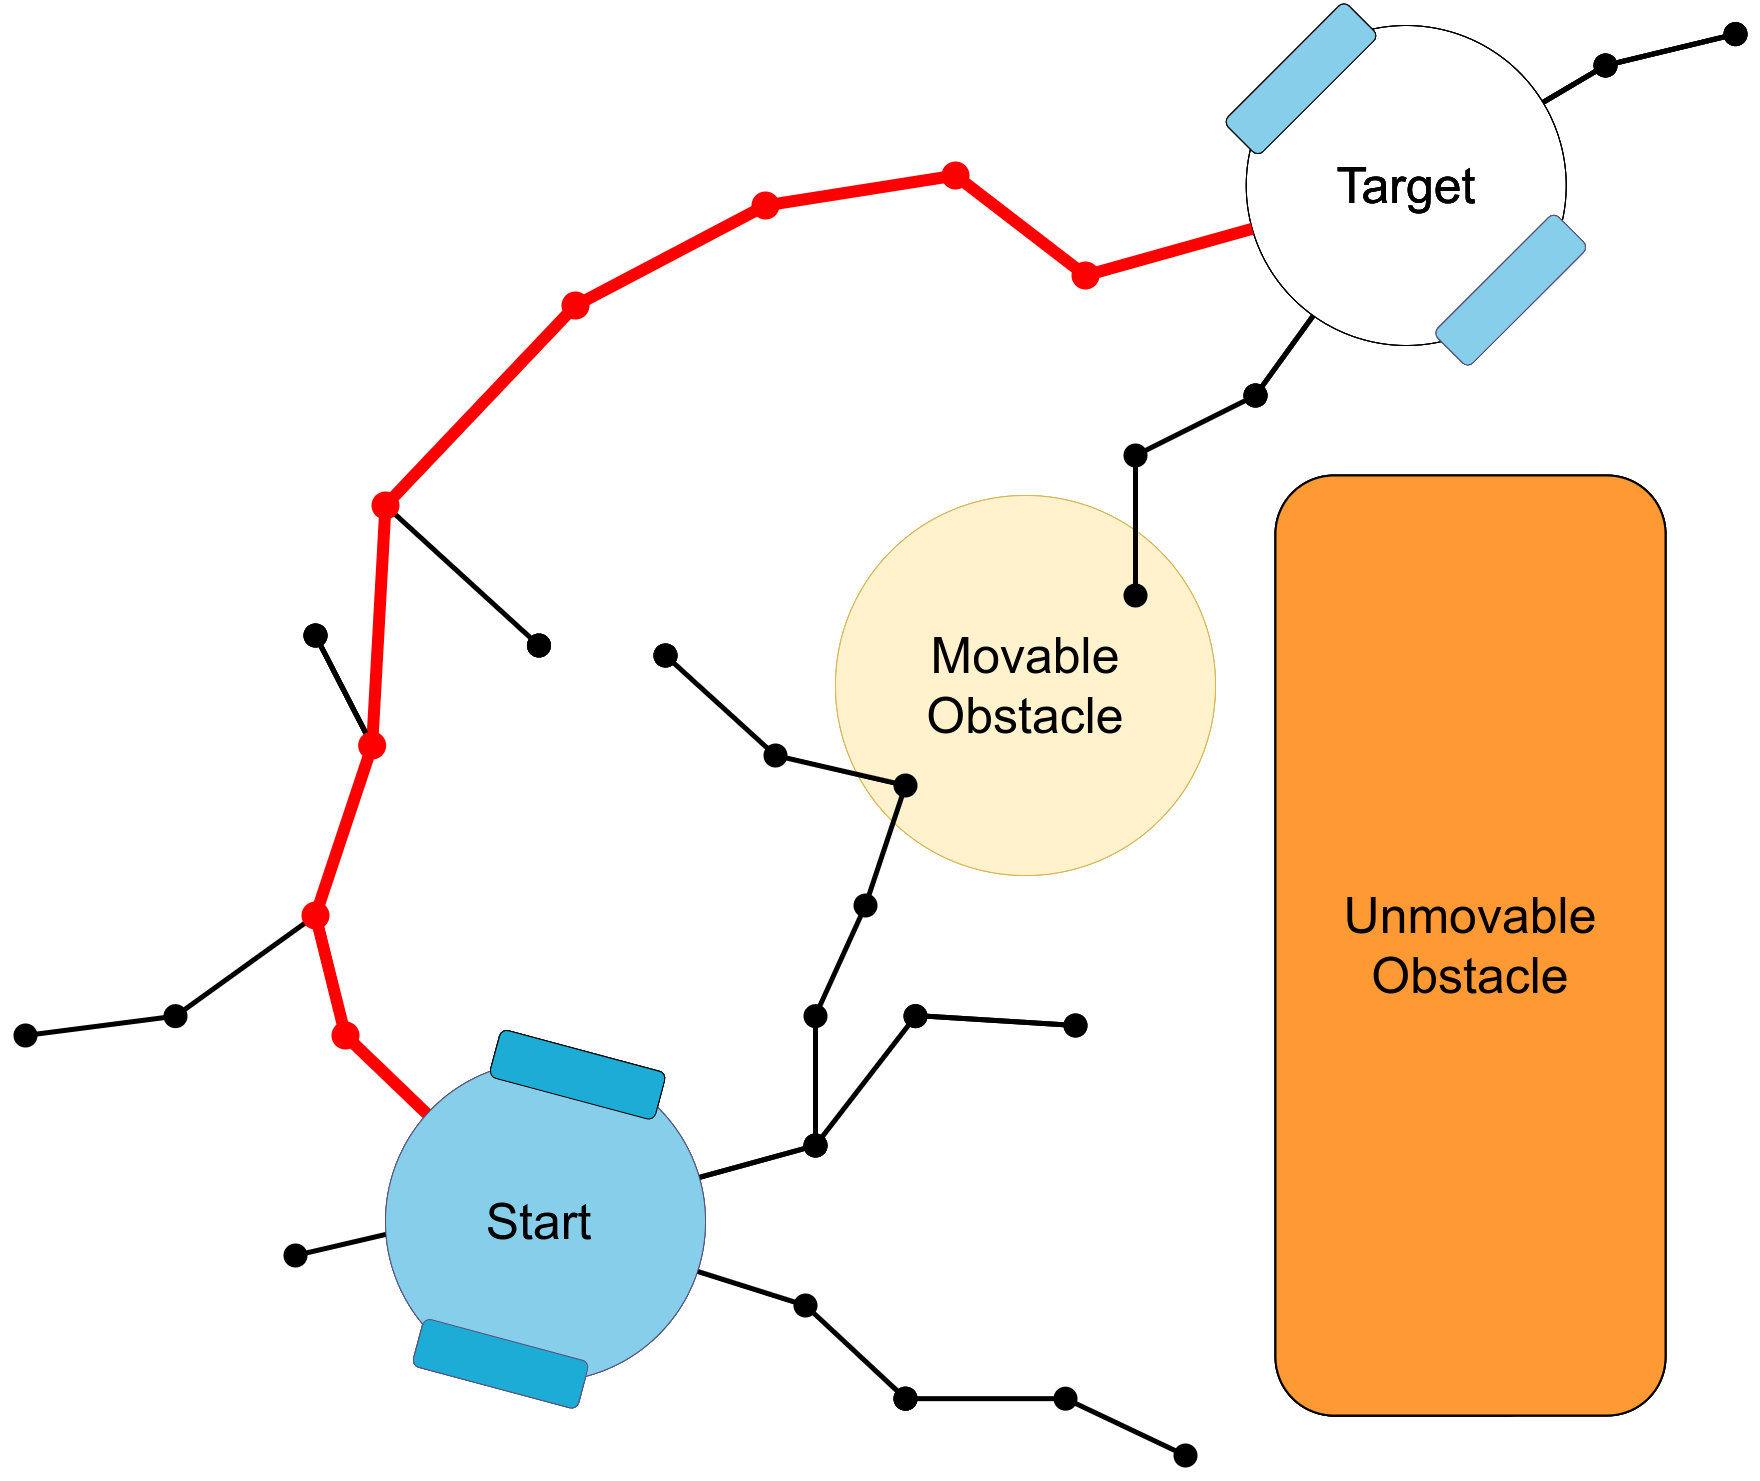
\includegraphics[width=0.75\textwidth]{figures/mp/7mp_path_found.drawio.png}
    \caption{The resulting configuration space after sample in \cref{fig:motion_planner_adding_one_sample}\\ was added. The path found is marked in red}
    \end{subfigure}%
    \begin{subfigure}{.5\textwidth}
    \hspace{-0.7cm}
    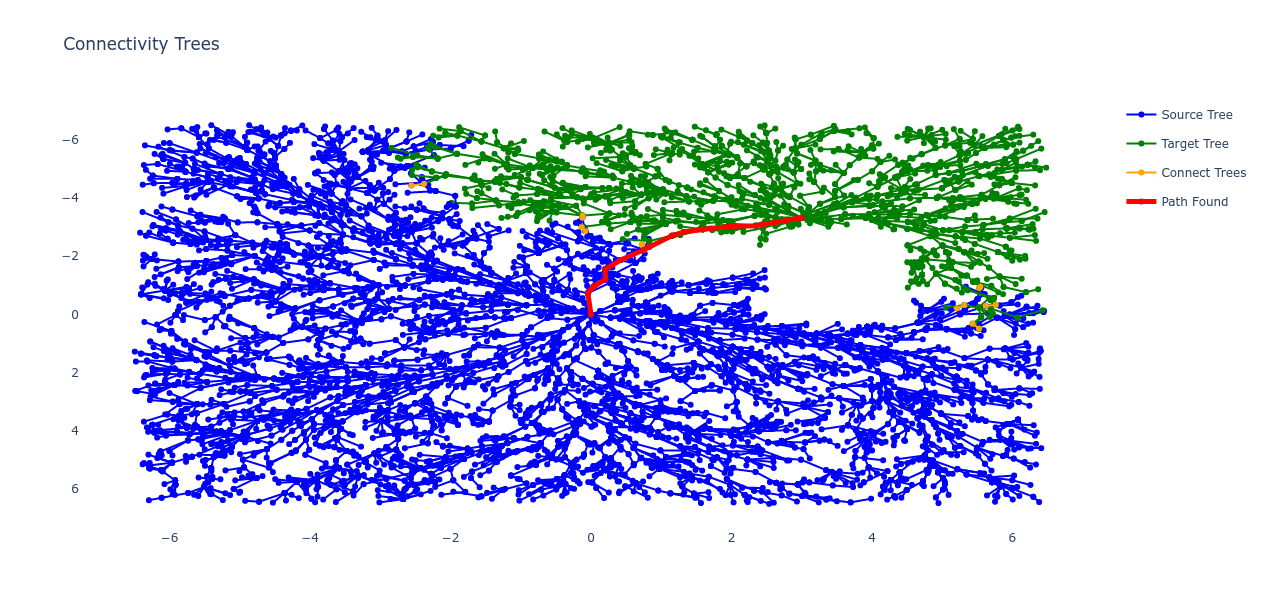
\includegraphics[width=1.1\textwidth]{figures/mp/mp_the_real_deal.png}
    \caption{A visualisation of the implemented \acs{RRT*} algorithm\\after a search from start to target}
    \end{subfigure}
    \label{fig:motion_planner_comparison}%
    \caption{Comparing schematic example to a visualisation of the real algorithm.}
\end{figure}

The result of adding an extra penalty for crossing unknown or movable subspace is that such subspaces are avoided if possible. If it is not possible to find a valid path, then movable or unknown subspaces are crossed, displayed in~\cref{fig:double_rrt_alg}. A path cannot be tracked by a controller if it crosses movable or unknown spaces, first, the object must be moved, and then the original path can be tracked. In~\cref{fig:double_rrt_alg} it can be seen that the motion planner cannot find a path around the movable object and is forced to add the cost to move the object. The added fixed cost for a path crossing through a movable or unknown object motivates the motion planner to find the shortest path around objects but prefers moving an object over making a large detour.\bs

\begin{figure}[H]
    \centering
    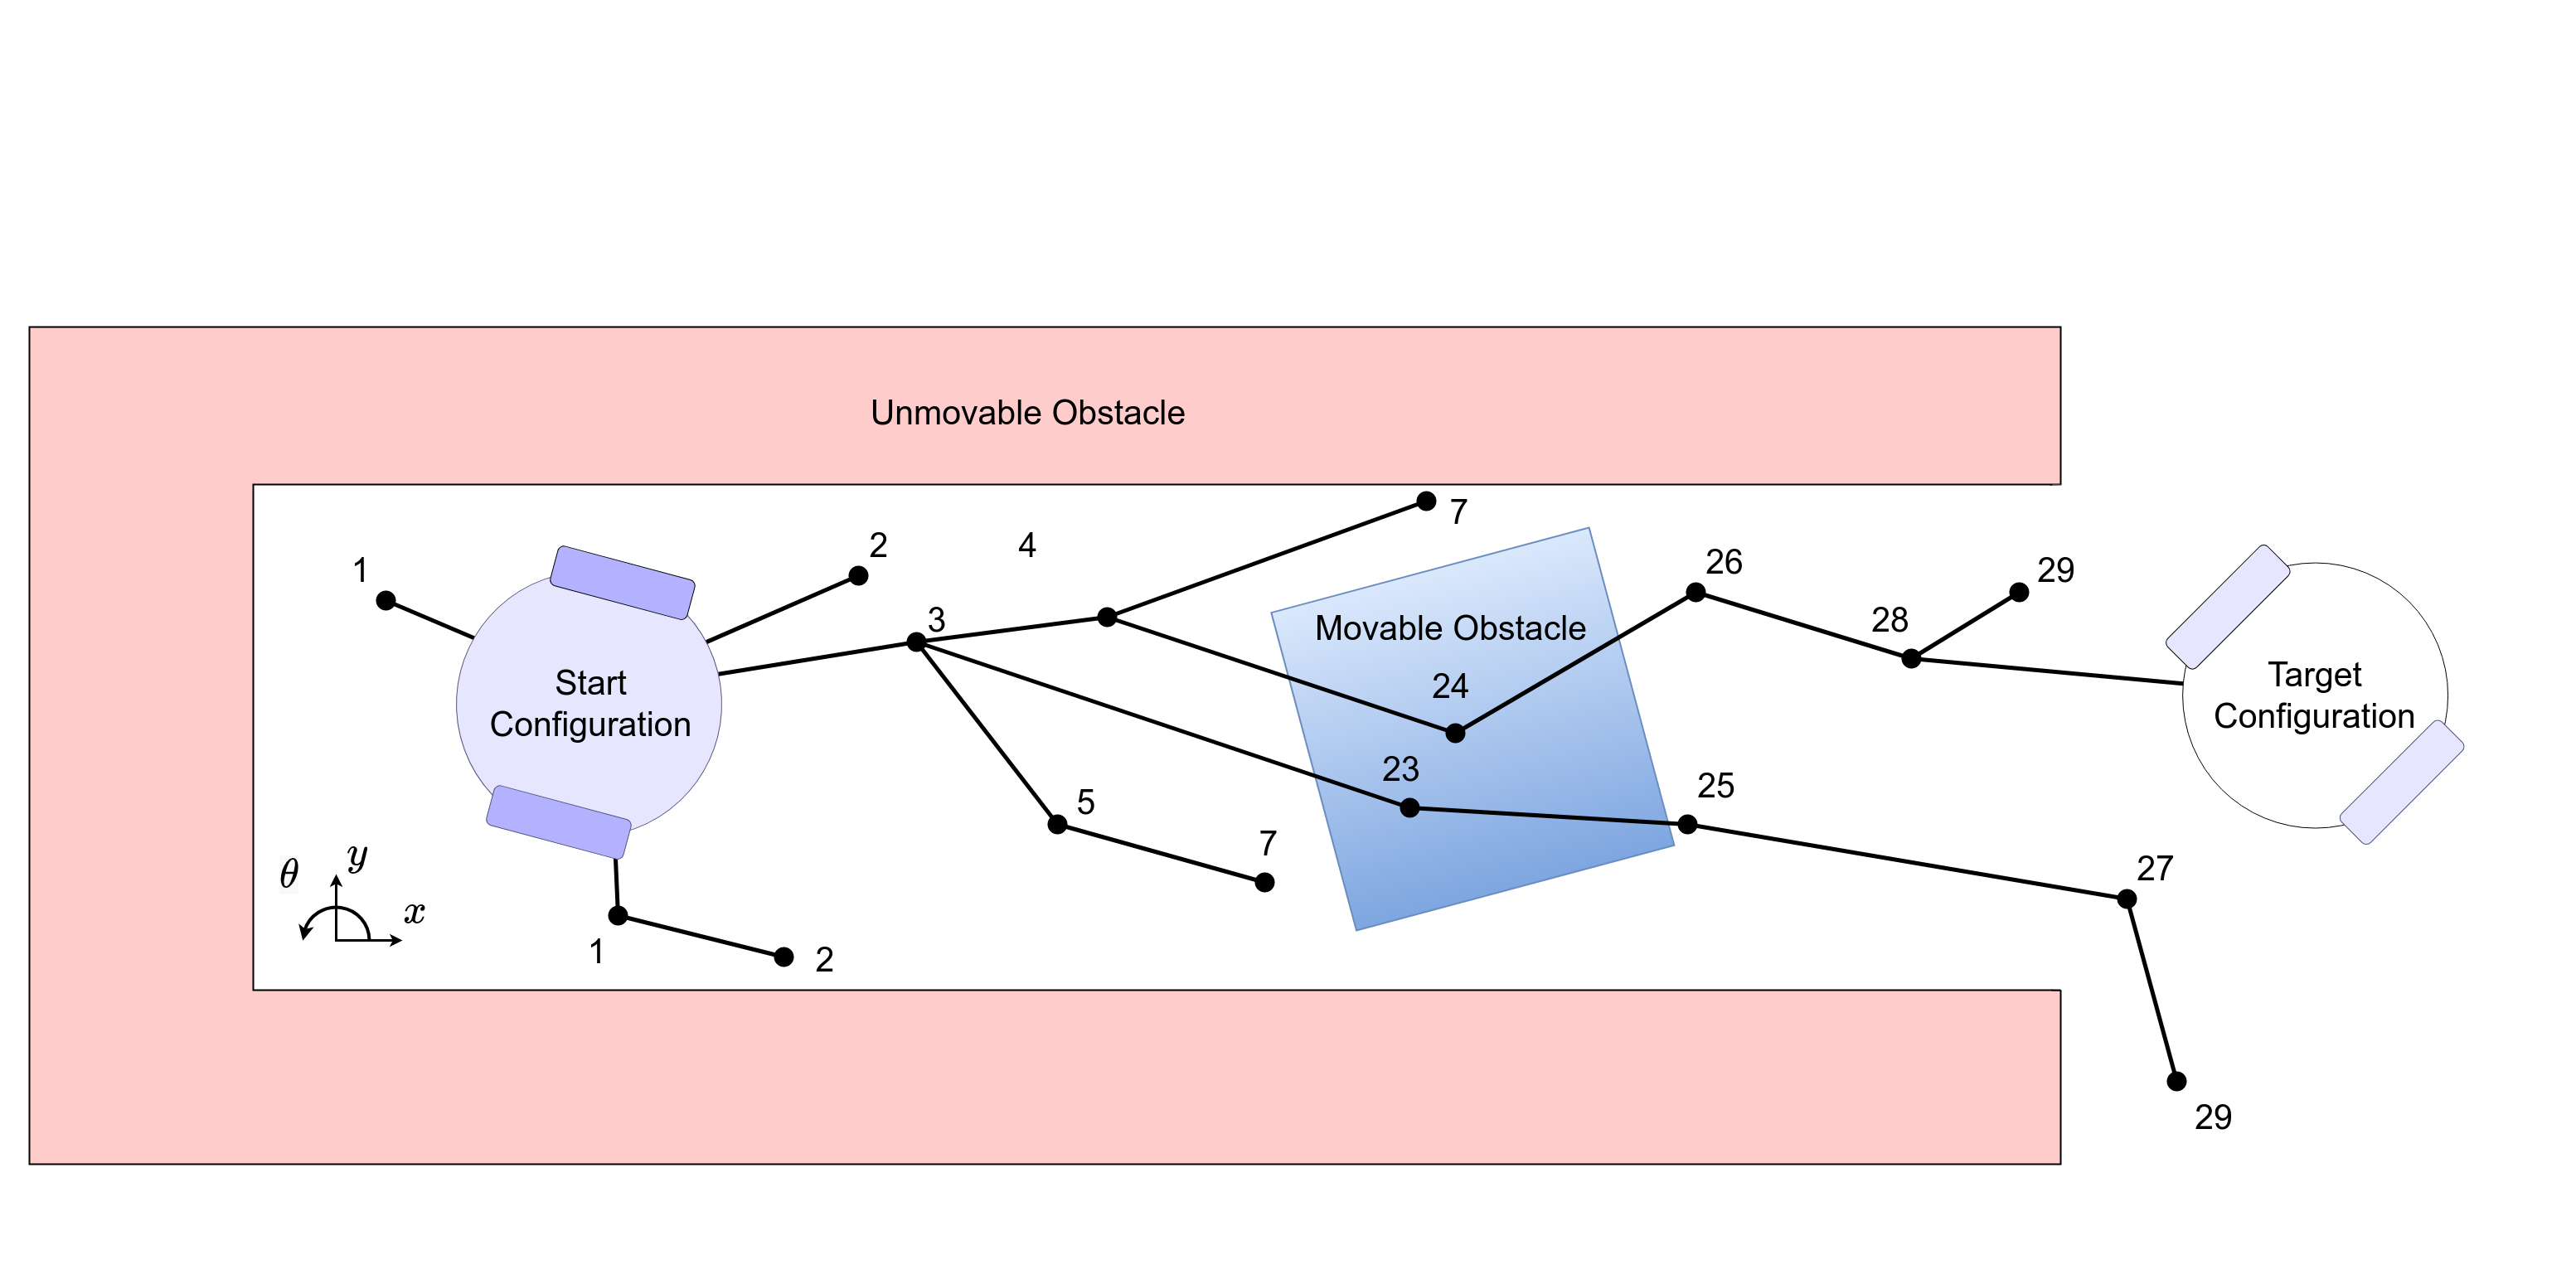
\includegraphics[width=0.9\textwidth]{figures/rrt_with_costs.png}
    \caption{Schematic view of the proposed double $\text{RRT}^*$ tree taking movable and\\unknown objects into account with cost to reach a sampled configuration displayed.}
    \label{fig:double_rrt_alg}
\end{figure}

The proposed motion planning algorithm searches the configuration space from the start connectivity tree and the target connectivity tree. Exploring faster compared to the single tree \ac{RRT*} algorithm. The proposed algorithm rewires nodes, resulting in lowering cost for existing paths. The proposed algorithm finds the optimal lowest-cost path with infinite sampling because of its ability to rewire nodes. The $LocalPlannerCheck$ provides feasible paths, such that the proposed algorithm yields paths that respect the system constraints. After all later on the system will be controlled to track the path. Now motion planning is discussed, manipulation will be discussed.

\subsection{Manipulation Planning}%
\label{subsec:manipulation_planning}
% Extending upon motion planning manipulation planning keeps track of 2 objects.
\todo[inline]{explain the manipulation planning extensions with a figure, no one is going to understand you otherwise.}
\todo[inline]{create manipulation planning subsection after implementation, code first, then write. Because writing is harder than coding}


\begin{figure}[H]
    \centering
    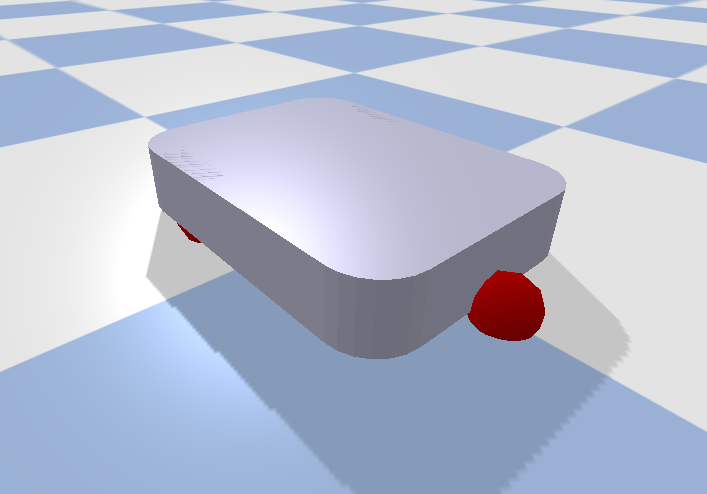
\includegraphics[width=5cm]{figures/boxer_robot}
    \caption{Speed comparison of increasingly difficult tasks}
    \label{fig:speed_comparison_planning}
\end{figure}

\section{Fault Detection}%
\label{sec:fault_detection}
During execution time, the \ac{hgraph} is unable to perform any action, such as motion planning or finding new hypotheses. This blocking behaviour has some implications, especially when an edge steers the system toward a target state and is blocked, for example, the controller steers the system to a target state, and meets an unmovable object. In such cases, the controller will never reach the target state and the system remains in a local minimum forever. Giving complete control to an edge is thus not desired because of the blocking behaviour of edges. More examples can be given such as system identification or push manipulation on an object that is cornered can be provided. However, instead of thinking of all possible options for how the robot could get stuck a more automated approach is sought.  A central coordinator who can step in and terminate the edge is desired. Detecting controller faults is a large robotic topic~\cite{khalastchi_fault_2019} properly implementing a fault detection and diagnosis module is out of the scope of this thesis. Instead, the two simple metrics will be monitored during execution. \ac{PE} where the predicted position is compared with the measured position of the system, and \ac{TE} where the path provided for the robot to track is compared with the trajectory that the robot made during tracking such a path. Definitions of \ac{PE} and \ac{TE} are now given, in \cref{table:monitoring_edge_metrics} insight is provided why a metric would catch certain faulty behaviour.

\todo[inline]{define \ac{PE}}
% Every time step a prediction one step into the future is made with the use of the dynamic model. Also, every time step the \ac{PE} is calculated, which is the difference between the one-step-ahead predictor of the previous timestep and the measurement of where the object currently is.
\todo[inline]{define \ac{TE}}

\subsection{Monitoring Metrics}

\begin{table}[htb!]
\centering
\begin{tabular}[t]{l p{10cm}}
  \acf{PE}&  During executing a sudden high \ac{PE} indicates unexpected behaviour occurs, such as when the robot has driven into an object which is was not expecting. A high \ac{PE}, which persists indicates that the robot is continuously blocked. Single collisions are allowed, but when the \ac{PE} exceeds a pre-defined threshold and persists over a pre-defined time, the \ac{hgraph} concludes that there was an error during execution and the edge failed.\\
  \acf{TE}& The system should not diverge too far from to path it is supposed to track, if the robot diverges more than a pre-defined threshold the \ac{hgraph} concludes that there was an error during execution and the edge fails. \\
\end{tabular}
\caption{Monitor metrics used to monitor if a fault occurred during execution of an edge}%
\label{table:monitoring_edge_metrics}
\end{table}



\chapter{The Hypothesis and Knowledge graph}%
\label{chap:hgraph_and_kgraph}

\textit{This chapter is dedicated to introducing and defining the proposed method, the proposed method consist of the \acl{halgorithm}, the \acl{hgraph} and the \acl{kgraph}. The \textbf{\acl{halgorithm}} acts on the \textbf{\acl{hgraph}} is responsible for searching the joint configuration space for action sequences to complete a specified task, \cref{subsec:hgraph_definition} is dedicated to the \ac{halgorithm} and the \ac{hgraph}. The \ac{halgorithm} additionally is responsible for collecting new knowledge of the environment. Gathered new environment knowledge is stored in the \textbf{\acl{kgraph}}, defined in \cref{subsec:kgraph_definition}. Collected knowledge is rated and ordered from \quotes{good} to \quotes{bad} experiences using various metrics. Such an ordering within collected knowledge makes the \ac{kgraph} a knowledge base that can be queried for action suggestions. \Cref{tikz:flowchart_proposed_method} presents a schematic overview of the interconnection of the knowledge-, hypothesis graph and the robot environment. A more in depth analysis of the hypothesis graph is given in~\cref{sec:hgraph}, and for the knowledge graph in~\cref{sec:kgraph}.}

\vspace{-0.2cm}
\begin{figure}[H] \centering
\begin{tikzpicture}[node distance = 2cm, auto]
    % Place nodes
    \node[draw=gray, rounded corners, inner sep=3ex, line width=7pt, fill=gray, fill opacity=0.4, minimum height=11.0cm, minimum width=5.8cm, yshift=3.25cm] (focusbox) {}; 
    \node[yshift=5.8cm, xshift=-1.5cm, align=left] at (focusbox) {\textbf{Thesis focus}};
   
   \node [outer sep=0cm] (environment) at (0,0)  {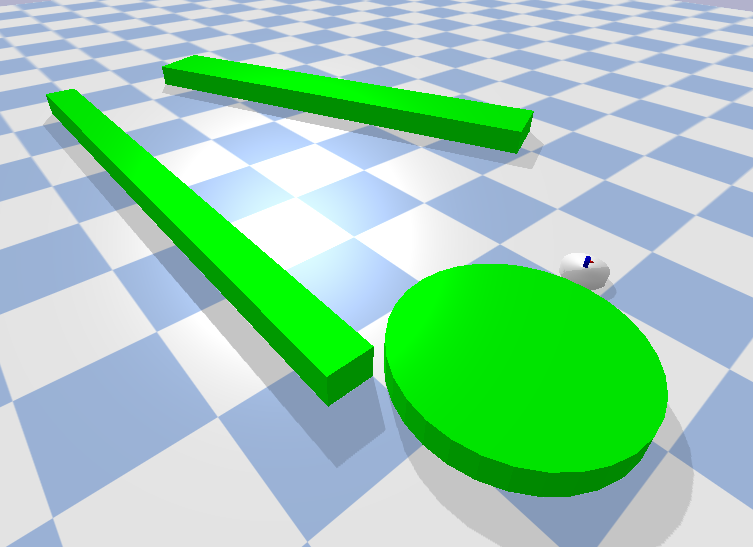
\includegraphics[width=4.6cm]{figures/example_environment.png}}; 

   \node [below, xshift=0.4cm, yshift=-.1cm, text width=5cm, align=left, outer sep=0cm] at (environment.north) {\textbf{Robot Environement}};
   
    \draw [myEvenLighterColor,
    rounded corners=0.3cm, 
    line width=0.3cm]  
    (environment.north west) -- 
    (environment.north east) --
    (environment.south east) --
    (environment.south west) -- cycle  ;
    
    \node [block,
    above of=environment,
    minimum height=2cm,
    minimum width=5cm,
    node distance=4.1cm,
    outer sep=0cm] (hgraph) {Hypothesis Algorithm};
   
    \node [block, 
    above of=hgraph, 
    node distance=3.3cm, 
    minimum width=5cm,
    minimum height=2.0cm] (kgraph) {Knowledge Graph};
      
    \node [rectangle, draw, 
    fill=myEvenLighterColor, 
    text width=5em, text centered, rounded corners, 
    right of=kgraph, 
    minimum width=4cm,
    minimum height=2cm,
    node distance=7.2cm] (ontology) {Ontology};
     
    \node [rectangle, draw, 
    fill=myEvenLighterColor, 
    text width=5em, text centered, rounded corners, 
    right of=hgraph, 
    minimum width=4cm,
    minimum height=2cm,
    node distance=7.2cm] (planner) {High-level planner};
    
    % Draw edges
    \draw[-stealth] ([yshift=0.155cm, xshift=0.4 cm]environment.north) -- node [xshift=-.05cm, right] {\shortstack[]{sensor\\measurements}}([xshift=0.4 cm]hgraph.south) ;
    \draw[-stealth] ([xshift=-0.4 cm]hgraph.south) -- node [left] {robot input}([yshift=0.155cm, xshift=-0.4 cm]environment.north) ;
    \draw[-stealth] (planner.west) -- node [pos=0.37, above] {task}(hgraph.east);
    \draw[-stealth] ([xshift=-0.4cm]kgraph.south) -- node [left] {\shortstack[]{action\\suggestions}}([xshift= -0.4cm]hgraph.north) ;
    \draw[stealth-] ([xshift=0.4cm]kgraph.south) -- node [right] {\shortstack[]{action\\feedback}}([xshift= 0.4cm]hgraph.north) ;
    \draw[-stealth] (kgraph.east) -- node [xshift=-0.1cm, above, pos=0.63] {\shortstack[]{environment\\knowledge}}(ontology.west);
    \draw[stealth-] ([xshift=0.4cm]ontology.south) -- node [right] {\shortstack[]{query}}([xshift=0.4cm]planner.north);
    \draw[-stealth] ([xshift=-0.4cm]ontology.south) -- node [left] {\shortstack[]{output}}([xshift=-0.4cm]planner.north);
    \draw[stealth-] (planner.south) |- ++ (2,-1) node[near end, above] {\shortstack[]{High-level\\task}};
    \end{tikzpicture}
\caption{Flowchart representation of the proposed method.}%
\label{tikz:flowchart_proposed_method}
\end{figure}

As the above figure shows, the thesis focus could be augmented with an ontology and high-level planner. Such an augmentation would create a framework capable of completing high-level tasks such as cleaning or exploring.\bs 

This chapter has terminology that is conveniently grouped in the following table.

\begin{table}[H]
\centering
\begin{tabular}[t]{l p{10cm}}
Task:   &  Tuple of objects and target configurations.\\
        & $\text{task} = \gls{task} = \left\langle \gls{objSet}_{\mathit{task}}, C_{\mathit{targets}} \right\rangle$\\
Subtask:& A single object, and a single target configuration.\\
        & $\text{subtask} = \gls{subtask}= \left\langle \mathit{obj}_{\mathit{subtask}}, \gls{c}_{\mathit{target}} \right\rangle$\\
Object Class & Classification assigned to an object.\\
             & $\gls{objectClass} = \textrm{Unknown}\vee \textrm{Obstacle}\vee \textrm{Movable}$\\
Node Status:& Status of a node indicates if a node is initialised, the \ac{halgorithm} was able to bring the object to the configuration or whether the \ac{halgorithm} fails to bring the object to its configuration.\\
            & \[\gls{nodeStatus} = \mathrm{Initialised} \vee \mathrm{Completed} \vee \mathrm{Failed} \]\\
Node:   & A node in the \acs{hgraph}, represents an object in a configuration with reachability indicated with a node status.\\
        & $\textrm{node} = \gls{node} = \left\langle \textrm{status}, \mathit{obj}, c \right\rangle$\\
Edge Status:& Status of a edge, elaborate information on the statuses can be found in \cref{tikz:status_action_edge}.\\
            & \[\gls{edgeStatus} = \mathrm{Initialised} \vee \mathrm{Path Exists} \vee \mathrm{System Model} \vee \] \[\mathrm{Path Planned} \vee \mathrm{Executing} \vee \mathrm{Completed} \vee \mathrm{Failed}\]\\
Edge:   & Edge connecting a node to another node in the \acs{hgraph} or \ac{kgraph}.\\
        & $ \textrm{edge} = \gls{edge} = \left\langle \textrm{status}, id_{\mathit{from}}, id_{\mathit{to}}, \textrm{verb}, \textrm{controller},\textrm{dynamic model}, \textrm{path}\right\rangle$\\
Hypothesis:& Sequence of successive edges in the \ac{hgraph}, an idea to put a object at it's target configuration. If executed and successfully completed, a subtask is completed.\\
           & $ \textrm{hypothesis} = \gls{hypothesis} = \left[\ \gls{edge}_{1}, \gls{edge}_{2}, \gls{edge}_{3}, \dots \gls{edge}_{m} \right]\ $, \hspace{0.5cm} $m>0$\\
Hypothesis Algorithm:& Graph based algorithm that searches for hypothesis in the \ac{hgraph} to complete subtasks eventually completing a task.\\
Hypothesis Graph:& Collection of nodes and edges. For every subtask a start and target node exist in the \ac{hgraph}, the \ac{halgorithm} searches for a path through nodes and edges to connect start to target node.\\
        & $ \textrm{\ac{hgraph}} = \gls{hgraph} = \left\langle \gls{nodesG}, \gls{edgesG} \right\rangle $\\
Knowledge Graph:& Collection of nodes and edges.  The \ac{kgraph} acts as a knowledge base and can be queried for an action suggestion.\\
        & $ \textrm{KGraph} = \gls{kgraph} = \left\langle \gls{nodesG}, \gls{edgesG} \right\rangle $\\
\end{tabular}
\caption{Terminology of terms used}
\label{table:proposed_method_terminology}
\end{table}

\section{Hypothesis Graph}%
\label{sec:hgraph}
The \ac{halgorithm} is responsible for generating action sequences, called hypothesis. An hypothesis consists of a list of successive edges in the \ac{hgraph} from start to target node in the \ac{hgraph}. When all subtasks in a task are completed, the \acf{halgorithm} halts and concludes the task successfully completed. A search in the joint configuration space is avoided because an edge only operates in a single mode of dynamics, such as driving or pushing. When an object cannot directly be steered toward its target location new nodes are generated which need to be completed before the original object can be steered toward its target location. An example of when an object cannot directly be steered toward its target state is because the path is blocked by another object. A hypothesis, consisting of a list of edges that represent actions in the robot environment might succeed or fail. \Cref{tikz:flowchart_hgraph} displays a flowchart explaining how new nodes and edges are generated in the \ac{hgraph}. Successfully completed edges eventually result in completed subtasks, failed edges trigger replanning that will restart the search to a hypothesis.\bs

The \ac{halgorithm} with the \ac{hgraph} have a familiar structure compared to some recent literature~\cite{ellis_navigation_2022,wang_affordancebased_2020}. An important distinction is that the proposed method in this thesis aims to combine the 3 topics: learning object dynamics, solving \ac{NAMO} problems and nonprehensile pushing. Recent literature is able to only combine one or two topics of the three.\bs

In the upcoming section the \ac{hgraph} is defined and discussed in \cref{subsec:hgraph_definition}. The \ac{halgorithm} is then discussed and in \cref{subsec:halgorithm}, where an explanation is provided on how the \ac{halgorithm} searches for a solution in the joint configuration space. The section is concluded with an extensive example.\bs

\subsection{Definition}%
\label{subsec:hgraph_definition}%
Before defining the \ac{hgraph}, some definitions are defined on which the \ac{hgraph} depends. First, recall the \textbf{state} defined in the \cref{sec:problem_description}.\bs

An object holds the information about an object.\\Formally, a \textbf{object},  $obst_{id}(k) = \left\langle s(k), shape \right\rangle $\bs

where $shape$ is linked to a 3D representation of the object which is used to construct the configuration space.\bs

An object node represents an object in a state.\\Formally, a \textbf{objectNode}, $V^{obst}_{id} =\left\langle \textrm{status}, obst(k)\right\rangle $\\where status indicates if the node has been visited in the \ac{hgraph}. $\textrm{status} = (Initialised, Completed, Failed)$\bs

An edge describes the details of how a node transitions to another node in the \ac{hgraph}. In the robot environment, an edge represents a change of state for an object. System identification and performing an action such as pushing or driving both change the state of objects in the robot environment, but because are very different, the edges are split into 2 categories. IdentificationEdges that collect system \ac{IO} data and convert that into a system model. And actionEdges that plan and track a motion from a start to a target state. Formally:\bs

A \textbf{identificationEdge},
\todo[inline]{define identificationEdge, currently hard coded models are used in the implementation}

A \textbf{actionEdge}, $\tau_{(from, to)} = \left\langle \textrm{status}, id_{from}, id_{to}, \textrm{verb}, \textrm{controller},\textrm{dynamic model}, \textrm{path}\right\rangle$\bs

with $id_{from}$ and $id_{to}$ indicating the node id of the node in the \ac{hgraph} where the edge start from and point to respectively, $verb$ an English verb describing the action the edge represents, the controller contains the controller used for driving the robot, the dynamic model is the dynamic model used by the controller, path a list of configurations indicating the path connecting a start- to target node.\bs
\todo[inline]{Martijn: what does this mean: "the controller contains the controller..."?}

A $verb = \{\textrm{driving, pushing}\}$.\bs

Now the nodes and edges have been defined, the \ac{hgraph} can be defined.\bs

Formally, a \textbf{hypothesis graph}, $G^{hypothesis} = \left\langle V, E \right\rangle $ 
\\comprising $V = \{V^{ob}_{i}\}$, \quad $E \in \{\tau_{(i,j)}| V_i, V_j \in \{V^{ob} \}, i \neq j\}$.\bs

Most \ac{hgraph} components have now been defined. The status of an identification edge or action edge still remains undefined and requires some further explanation.\bs

\paragraph{Status, Types and Lifetime of edges}
Because system identification and tracking a path are so very different, the edges are split into two categories, identification edges and action edges. An identification edge, which is responsible for sending an input sequence to the system and recording the system output. That input/output sequence and assumptions on the system are the basis for system identification, techniques on various system identification methods are discussed in \cref{sec:sys_iden}. The goal is to create a dynamical model which is augmented with a corresponding controller is closed-loop stable.\bs

An identificationEdge, the status can be visualised in \cref{tikz:status_identification_edge}.\bs

\begin{figure}[H]
\centering
\begin{tikzpicture}[node distance = 2cm, auto, initial]
    \node [state, fill=my_dark_blue] (init_test_num) {IT\#t};
    \node [state, fill=my_light_blue, below of=init_test_num] (completed_test_num) {CT\#t};
    \node [state, accepting, fill=my_green, below of=completed_test_num] (completed) {CO};
    \node [state, accepting, fill=my_red, right of=completed_test_num, node distance=6cm] (failed) {FAIL};

 % arrows
    \draw [-stealth] ([xshift=-2cm]init_test_num.west) to node[near start,above]{\shortstack[]{select compatible\\sys. iden. method}} (init_test_num.west);
    \draw[-stealth] (init_test_num) edge[bend right] node[left]{Collect \ac{IO} data} (completed_test_num)
(completed_test_num) edge node[left]{create system model} (completed);
    \draw [-stealth] (completed_test_num) edge[bend right] node[right]{goto next start state} (init_test_num);
    \draw [-stealth] (completed_test_num) to node[]{Unable to reach next start state}  (failed.west);
    \draw [-stealth] (init_test_num) [out=0, in=90] to node[above]{Unable to reach next pos}  (failed.north);

\end{tikzpicture}
\caption{\acs{FSM} displaying the status of an identification edge}%
\label{tikz:status_identification_edge}
\end{figure}

\todo[inline]{some explainer on this status of iden edge}

The second type of edge is an actionEdge, containing a drive or push action. An actionEdge ready for execution contains all the necessary information to send input to the robot resulting in an object being steered toward it's target state. Before an edge is ready for execution it should be initialised properly, more specifically: initialised, path estimated should be performed, a system model must be initiated and path planning must be performed. Then finally the edge is ready to be executed and send input toward the robot, an \ac{FSM} of the actionEdge's status can be visualised in \cref{tikz:status_action_edge}.\bs

\begin{figure}[H]
\centering
\begin{tikzpicture}[node distance = 2cm, auto, initial]
    % \node [state, fill=lavenderIndigo] (init) {IN};
    \node [state, fill=my_purple] (init) {IN};
    \node [state, fill=my_dark_blue, below of=init] (path_exist) {PE};
    \node [state, fill=my_light_blue, below of=path_exist] (system_model) {SM};
    \node [state, fill=my_green, below of=system_model] (path_planned) {PP};
    \node [state, fill=my_yellow, below of=path_planned] (executing) {EX};
    \node [state, accepting, fill=my_orange, below of=executing] (completed) {CO};
    \node [state, accepting, fill=my_red] (failed) at ([xshift=4cm]$(system_model)!0.5!(path_planned)$) {FAIL};
    
 % arrows
    \draw [-stealth] ([xshift=-2cm]init.west) to node[near start,above]{select controller} (init.west);
    \draw[-stealth] (init) edge node[left]{graph-based path estimation} (path_exist)
      (path_exist) edge[bend right] node[left]{load in system model} (system_model)
(system_model) edge[bend right] node[left]{motion planning} (path_planned)
(path_planned) edge[bend right] node[left]{goto execution loop} (executing)
(executing) edge[bend right] node[left]{completed} (completed);

    \draw [-stealth] (init.east) [out=0, in=90] to node[xshift=0.1cm, right]{path non-existence proven}  ([yshift=-0.03cm,xshift=0.2cm]failed.north);
    \draw [-stealth] (path_exist.east) [out=0, in=90] to node[xshift=-0.6cm,yshift=0.55cm, above]{\shortstack[l]{system\\identification\\error}}  ([yshift=-0.03cm,xshift=-0.2cm]failed.north);
    \draw [-stealth] (system_model.east) [out=0, in=180] to node[xshift=0.1cm, yshift=0.3cm, above]{\shortstack[l]{motion\\planning\\error}} (failed.west);
    node[right]{motion planning error}  
    ([yshift=-0.3cm]failed.west);
    \draw [-stealth] (executing.east) [out=0, in=-90] to node[xshift=0.1cm,right]{fault detected}(failed.south);

\end{tikzpicture}
\caption{\acs{FSM} displaying the state of an action edge}%
\label{tikz:status_action_edge}
\end{figure}

% \par\smallskip\noindent
\centerline{\begin{minipage}{0.8\textwidth}
\begin{enumerate}
  \item[INITIALISED (IN)] The edge is created with a source and target node which are present in the \ac{hgraph}. A choice of controller is made.
    \item[PATH EXISTS (PE)] A graph-based search is performed to validate if the target state is reachable assuming that the system is holonomic.
    \item[SYSTEM MODEL (SM)] A dynamics system model is provided to the controller residing in the edge.
    \item[PATH PLANNED (PP)] Resulting from a sample-based planner, a path from start to target state is provided. 
    \item[EXECUTING (EX)] The edge is currently receiving observations from the robot environment and sends back robot input. 
    \item[COMPLETED (COMPL)] The edge has driven the system toward its target state and its performance has been calculated.
    \item[FAILED (FAIL)] An error occurred, yielding the edge unusable. 
\end{enumerate}
\end{minipage}}
\par\smallskip

\Cref{tikz:status_action_edge} shows that many steps must successfully be completed before the robot can start executing. The performance of an edge during execution, measured in various metrics (\cref{sec:proposed_method_metrics} is dedicated to metrics) is dependent on many aspects. Such as the choice of controller, the path estimation, the system model yielded by the identification edge and the path yielded by motion planning. Now that he \ac{hgraph} is defined, let's see how it is generated in the upcoming section.\bs

\subsection{\acl{halgorithm}}%
\label{subsec:halgorithm}
This section will provide a mathematical description of the proposed \ac{halgorithm}, the search and execution loop are discussed. The section will finalise with 4 examples. First, let's look into the math of the \ac{halgorithm}.\bs

\todo[inline]{a mathematically solid describtion of your backward search algorithm}

During a backward search, edges are added pointing toward the target node (or to nodes that point toward the target node). Trying to connect the robot node through a list of succesive directed edges to a target node. If such a path has been found in the \ac{hgraph}, a hypothesis has been found and the robot can start executing edges.

A flowchart of the \ac{halgorithm} is presented in \cref{tikz:flowchart_hgraph}. Compared to the mathematical description of the \ac{halgorithm} the flowchart provides more detail, including an eleborate description for every block in the flowchart (see \cref{table:explainer_hgraph_figures_nodes}). The flowchart includes path estimation, planning and the behavior when failure occures. A connection point to the \ac{kgraph} and robot environment are included. The blocks in the flowchart indicate which action they take and where, such as the configuration space, the \ac{kgraph} or the \ac{hgraph}. With the flowchart is straigtforward to see how the \ac{halgorithm} connects to the status of edges, with the mathematical description of the \ac{halgorithm} that is harder so see. Compared to the flowchart the mathematical description is a abstacted version, leaving many details out that are related to the robot in this thesis. An abstracted mathematical description is simpler and encompasses a broader field of robots. So could the mathematical description also be applied to another robot such as a movable robot with robot arm and gripper. The flowchart encompasses to many details to be applied after such an change in robot hardware. 

\input{mainmatter/hypothesis_graph/hgraph_tikz_figure}

\begin{table}[H]
\centering
\rowcolors{2}{white}{myLightColor}
\begin{tabular}[t]{>{\raggedright}p{3.5cm}>{\raggedright\arraybackslash}p{10.5cm}}
  \textbf{Node name} & \textbf{Description of actions taken}\\\toprule
  Task Finished & log all metrics for the \ac{hgraph}, then deconstruct \ac{hgraph}.\\
  Create Start and\newline Target Nodes & Generate a robot node and the start and target nodes for every subtask in the task.\\
Update Current Subtask & Select an unfinished subtask or update current subtask. Use the backward search technique. The \textit{current\_start\_node} and \textit{current\_target\_node} are updated. When all subtask have been addressed, conclude task is finished. \\
Estimate Path\newline Existence & Check if a path exists between \textit{current\_start\_node} and \textit{current\_target\_node} whilst assuming that the object is holonomic.\\
Add Node to\newline Drive to Object & Add a node before the \textit{current\_target\_node}.\\
Unfeasible Node & Update node's status to unfeasible because is can not be completed, log failed Edge.\\
Knowledge Available& Query the \ac{kgraph} for action suggestion to connect \textit{current\_target\_node} to \textit{current\_target\_node}\\
Knowledge Usable& Check if a suggested action is not on the blacklist.\\
Object Movable & Check if object is classified as movable\\
Robot Close to Object& Check if the object is inside directly reachable free space of the robot \\
Generate Random\newline Action& Randomly sample a controller with a compatible system identification method that is not on the blacklist. \\
All Possible Actions Failed & Every possible action is on the blacklist for the \textit{current\_target\_node}, update \textit{current\_target\_node} status to failed.\\
Add Drive System Identification Edge & Adds identification edge between a newly generated node and the drive action edge source node. \\
Model Available& Checks if the drive action edge contains a system model. \\
Action Type& Checks the action type. \\
Model Available& Checkif the push action edge containts a system model. \\
Add Push System\newline Identification Edge& Adds identification edge compatible with push action edge. \\
Motion Planning& Search a path for the \textit{current\_edge}, detect blocking objects. \\
Add Node to Free Path & Search closeby pose for object to free path. Create node to push object toward that pose. \\
Manipulation Planning & Search a path for the \textit{current\_edge}, detect blocking objects.\\
Add Node to Drive\newline to Push Pose& Create node to drive toward push pose, add before action edge. \\
Robot Close to\newline Push Pose & Check if the robot is overlapping with the best push position. \\
Path to Target& Is there a path from robot to target node in the \ac{hgraph}, then set first edge to \textit{current\_edge} otherwise update subtask.\\
First Action Planned&  Check if motion/manipulation planning was performed. \\
Execute& Execute the \textit{current\_edge}, update \ac{hgraph} after completion, log failed hypothesis if a fault is detected. \\
Subtask Succesfully\newline Completed& Log hypothesis metrics. \\
Target Node Reached& Check if the target node is reached.\\
\end{tabular}
\caption{Eleborate information on actions taken by blocks in \cref{tikz:flowchart_hgraph}.}%
\label{table:explainer_hgraph_figures_nodes}
\end{table}

When all tuning parameters are set, the \ac{hgraph} is initialized and a task is provided, there is only a single access point toward the \ac{hgraph}. A function \textit{respond(observation)} that provides the \ac{halgorithm} with sensor measurements of the environment with the argument \textit{observation}. The function \textit{respond($\cdot$)} returns control in put for the robot. In this theses, the sensor measurements are the configuration of objects in the environment. Recall that the perfect-sensor assumption, assumption~\ref{assumption:perfect_object_sensor} that makes access to the exact configuration of every object possible.\bs


\paragraph{The Blacklist}%
Undesirable behavior is to generate an edge that fails, only to regenerate and fail again. This infinite behavior is prevented by the blacklist. When the \ac{halgorithm} connects two nodes with an action edge, the possible parameterizations (controller and system model) are filtered. Thus any parameterisation that is on the blacklist for this specific node (to which the action edge would point toward) cannot be created again for the lifetime of the \ac{hgraph}. An example where the blacklist can be seen in action is \cref{fig:failure_in_hgraph}.\bs

\todo[inline]{math def for blacklist on the nodes}


\subsection{The Search and the Execution loop}%
\label{subsec:two_loops}
In \cref{tikz:flowchart_hgraph} two main loops can be identified, see \Cref{fig:two_loops_identified}. These loops are the search loop, and the execution loop.\bs

\begin{figure}[H]
    \centering
    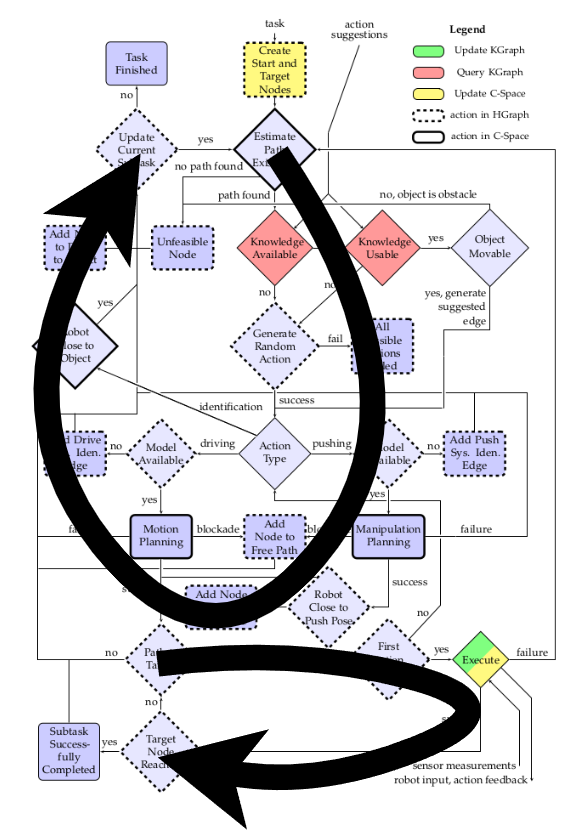
\includegraphics[width=7cm]{figures/two_loops_identified}
    \caption{The search (above) and execution (below) loop.}%
    \label{fig:two_loops_identified}
\end{figure}

Whilst the \ac{halgorithm} resides in the search loop, hypotheses are formed. Forming a hypothesis generates nodes, edges, and progressing their status as described in \cref{tikz:status_identification_edge,tikz:status_action_edge}. In the execution loop \textit{an edge is being executed}, a phrase to describe that the controller residing in an edge is sending control input toward the robot. The \ac{halgorithm} operates synchronously, thus at any point in time, the \ac{halgorithm} resides in a single block within \cref{tikz:flowchart_hgraph}. The result is that the robots cannot operate whilst the \ac{halgorithm} resides in the search loop, and during execution, no hypothesis can be formed or updated. Assumption~\ref{assumption:closed_world} guarantees that the robot environment does not change causing existing hypotheses to be outdated.\bs

\subsection{Examples}%
\label{subsec:hgraph_example}

Before displaying example \ac{hgraph}'s a legend is now presented.\bs

\begin{figure}[H]
    \centering
    \begin{subfigure}{0.2\textwidth}
    \centering
    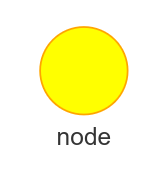
\includegraphics[width=0.7\textwidth]{figures/connecting_nodes/legend/node}
    \caption{Regular node created by the \ac{halgorithm}.\newline}%
    \end{subfigure}
    \begin{subfigure}{0.2\textwidth}
    \centering
    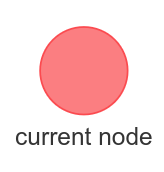
\includegraphics[width=0.7\textwidth]{figures/connecting_nodes/legend/current_node}
    \caption{Current node indicates that it's outgoing edge is now or is next to be executed.}%
    \end{subfigure}
    \begin{subfigure}{0.2\textwidth}
    \centering
    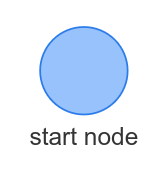
\includegraphics[width=0.7\textwidth]{figures/connecting_nodes/legend/starting_node}
    \caption{Starting node, one is generated at for every subtask.}%
    \end{subfigure}
    \begin{subfigure}{0.2\textwidth}
    \centering
    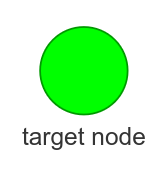
\includegraphics[width=0.7\textwidth]{figures/connecting_nodes/legend/target_node}
    \caption{Target node, one is generated for every subtask.\newline}%
    \end{subfigure}

    \begin{subfigure}{0.33\textwidth}
    \centering
    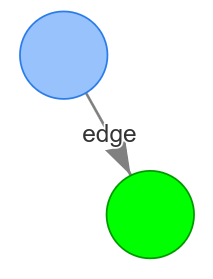
\includegraphics[width=0.7\textwidth]{figures/connecting_nodes/legend/edge}
    \caption{Edge with status IN, PE, SM, PP or EX.}%
    \end{subfigure}
    \begin{subfigure}{0.33\textwidth}
    \centering
    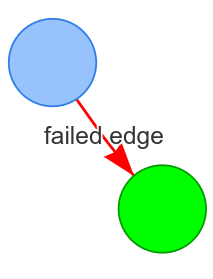
\includegraphics[width=0.7\textwidth]{figures/connecting_nodes/legend/failed_edge}
    \caption{Edge with status FAILED (FAIL)}%
    \end{subfigure}
    \begin{subfigure}{0.33\textwidth}
    \centering
    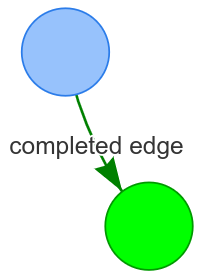
\includegraphics[width=0.7\textwidth]{figures/connecting_nodes/legend/completed_edge}
    \caption{Edge with status COMPLETED (CO)}%
    \end{subfigure}
    \caption{Legend for \ac{hgraph}'s nodes an edges}%
    \label{fig:hgraph_legend}
\end{figure}

\paragraph{Driving and Pushing} Four examples are presented, starting with a driving task in \cref{fig:robot_drive_hgraph}, then a pushing task in \cref{fig:robot_push_hgraph}.\bs

\begin{figure}[H]
    \centering
    \begin{subfigure}{.3\textwidth}
    \centering
    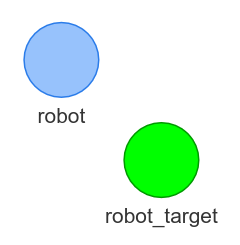
\includegraphics[width=0.7\textwidth]{figures/connecting_nodes/robot_to_target/robot_to_target}
    \end{subfigure}
    \begin{subfigure}{.3\textwidth}
    \centering
    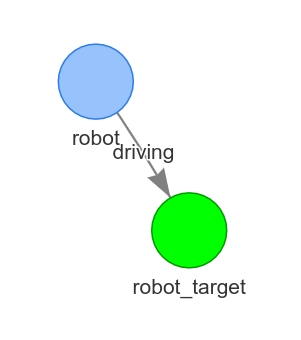
\includegraphics[width=0.9\textwidth]{figures/connecting_nodes/robot_to_target/robot_drive_target}
    \end{subfigure}
    \begin{subfigure}{.3\textwidth}
    \centering
    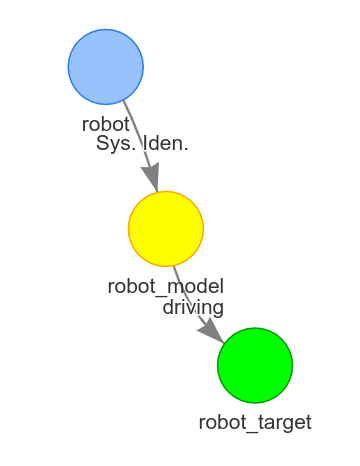
\includegraphics[width=\textwidth]{figures/connecting_nodes/robot_to_target/robot_iden_drive_target}
    \end{subfigure}
    \caption{\ac{hgraph} generated by the \ac{halgorithm} to drive the robot to a target configuration}%
    \label{fig:robot_drive_hgraph}
\end{figure}

The robot does not have a system model of itself, thus first system identification must be performed before it can drive to the specified target configuration. The \ac{kgraph} that will be discussed in \cref{subsec:kgraph_definition} can suggest an action that includes a system model. In that case, system identification is not needed. The following figure displays succesfully executing the hypothesis found in \cref{fig:robot_drive_hgraph}.\bs

\begin{figure}[H]
    \centering
    \begin{subfigure}{.3\textwidth}
    \centering
    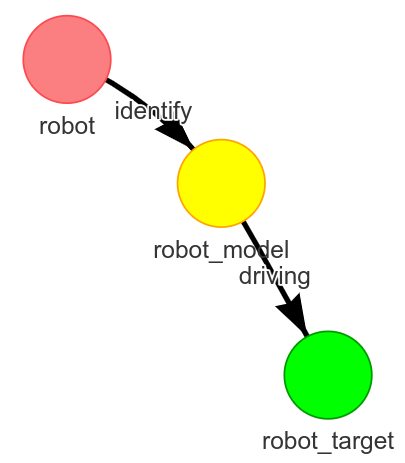
\includegraphics[width=0.8\textwidth]{figures/connecting_nodes/robot_to_target/execute_robot_to_target_1}
    \end{subfigure}
    \begin{subfigure}{.3\textwidth}
    \centering
    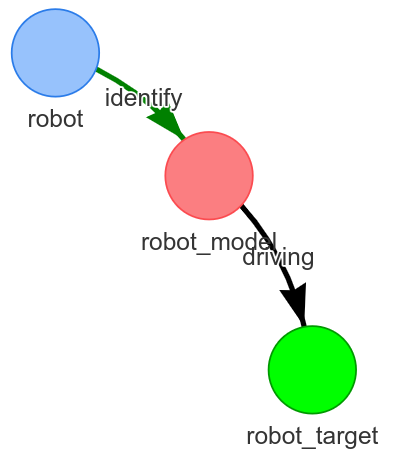
\includegraphics[width=0.8\textwidth]{figures/connecting_nodes/robot_to_target/execute_robot_to_target_2}
    \end{subfigure}
    \begin{subfigure}{.3\textwidth}
    \centering
    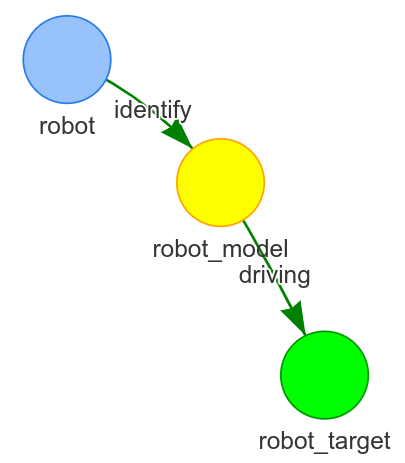
\includegraphics[width=0.8\textwidth]{figures/connecting_nodes/robot_to_target/execute_robot_to_target_3}
    \end{subfigure}
    \caption{Executing the hypothesis found in \cref{fig:robot_drive_hgraph}.}
    \label{fig:execute_robot_to_target}
\end{figure}

Upcoming figure will display the hypothesis generated to push an object to a target position. Both generating a hypothesis and executing the hypothesis are intertwined, this is because certain information should first be collected from the environment before the full hypothesis can be generated. An example is the \textit{best\_push\_position} that can be found in \cref{subfig:robot_push_7,subfig:robot_push_8,subfig:robot_push_9}. The \textit{best\_push\_position} can be found after manipulation planning for the pushing edge is completed. For motion planning a system model is required, thus the corresponding system identification edge should be completed before manipulation planning can start, and than the \textit{best\_push\_position} can be determined.\bs

\begin{figure}[H]
    \centering
    \begin{subfigure}{.3\textwidth}
    \centering
    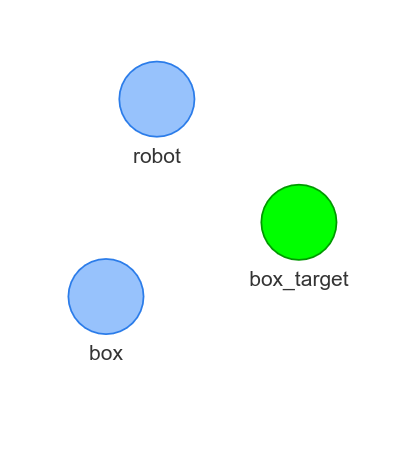
\includegraphics[width=0.8\textwidth]{figures/connecting_nodes/robot_push/robot_push_1}
    \caption{}
    \end{subfigure}
    \begin{subfigure}{.3\textwidth}
    \centering
    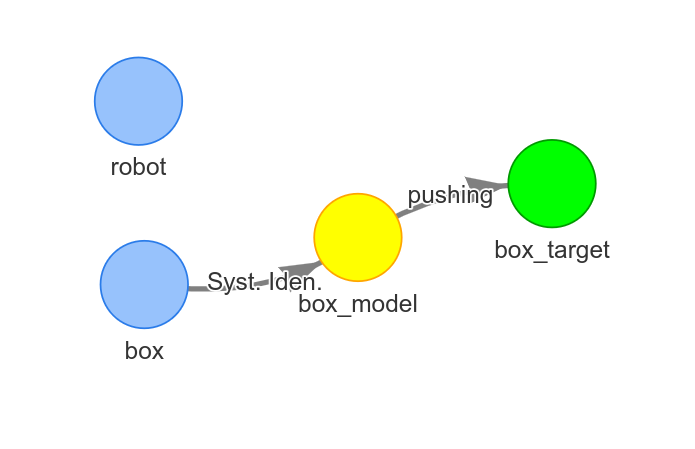
\includegraphics[width=1.1\textwidth]{figures/connecting_nodes/robot_push/robot_push_2}
    \caption{}\label{subfig:robot_push_2}
    \end{subfigure}
    \begin{subfigure}{.3\textwidth}
    \centering
    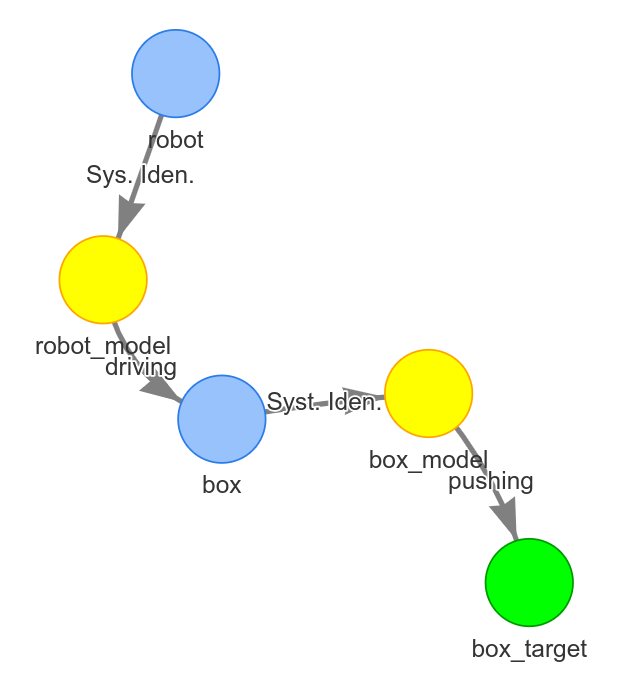
\includegraphics[width=1\textwidth]{figures/connecting_nodes/robot_push/robot_push_3}
    \caption{}\label{subfig:robot_push_3}
    \end{subfigure}

    \begin{subfigure}{.3\textwidth}
    \centering
    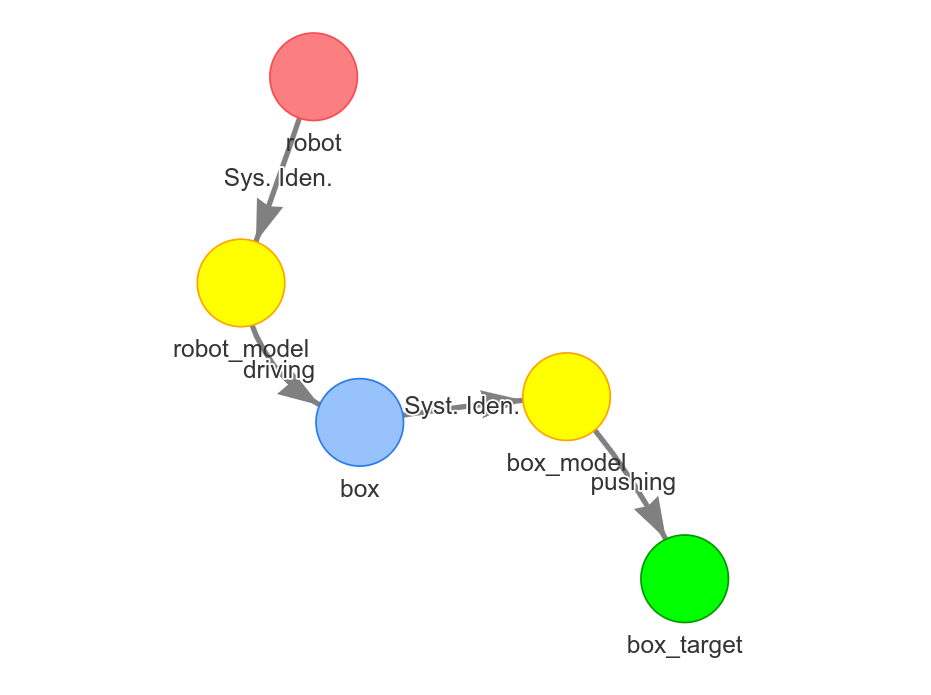
\includegraphics[width=1\textwidth]{figures/connecting_nodes/robot_push/robot_push_4}
    \caption{}\label{subfig:robot_push_4}
    \end{subfigure}
    \begin{subfigure}{.3\textwidth}
    \centering
    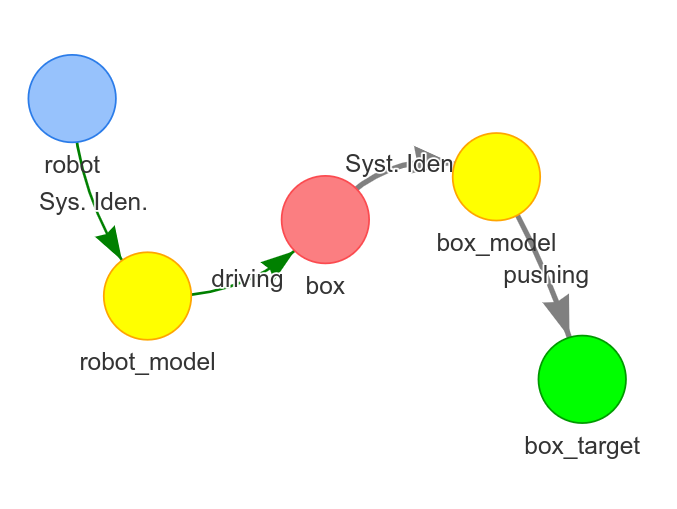
\includegraphics[width=1.05\textwidth]{figures/connecting_nodes/robot_push/robot_push_5}
    \caption{}\label{subfig:robot_push_5}
    \end{subfigure}
    \begin{subfigure}{.3\textwidth}
    \centering
    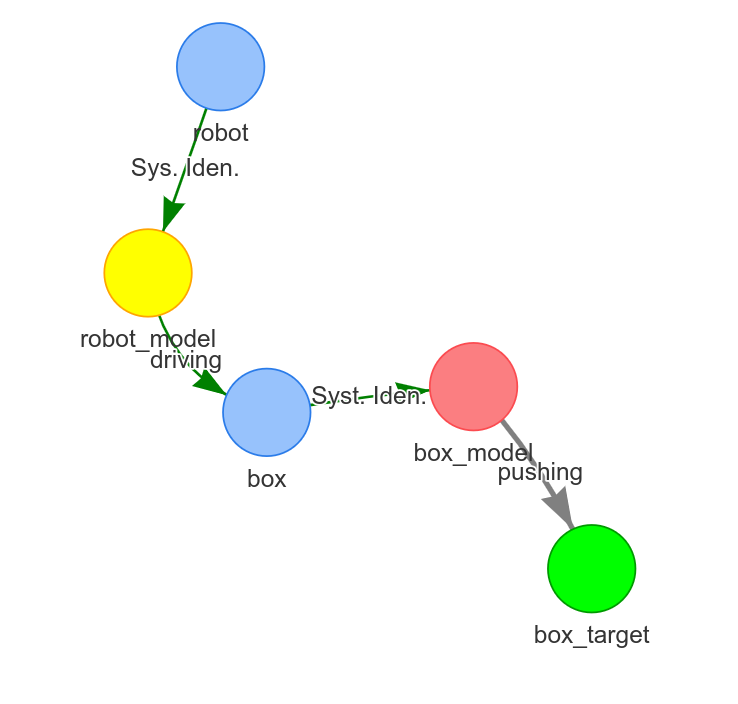
\includegraphics[width=1.05\textwidth]{figures/connecting_nodes/robot_push/robot_push_6}
    \caption{}\label{subfig:robot_push_6}
    \end{subfigure}

    \begin{subfigure}{.3\textwidth}
    \centering
    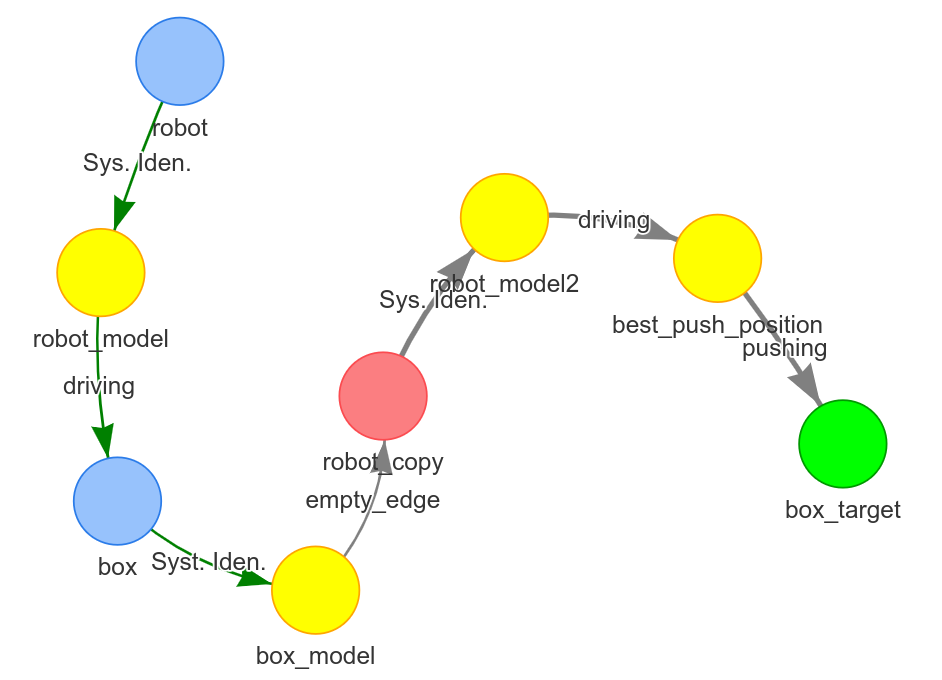
\includegraphics[width=1\textwidth]{figures/connecting_nodes/robot_push/robot_push_7}
    \caption{}\label{subfig:robot_push_7}
    \end{subfigure}
    \begin{subfigure}{.3\textwidth}
    \centering
    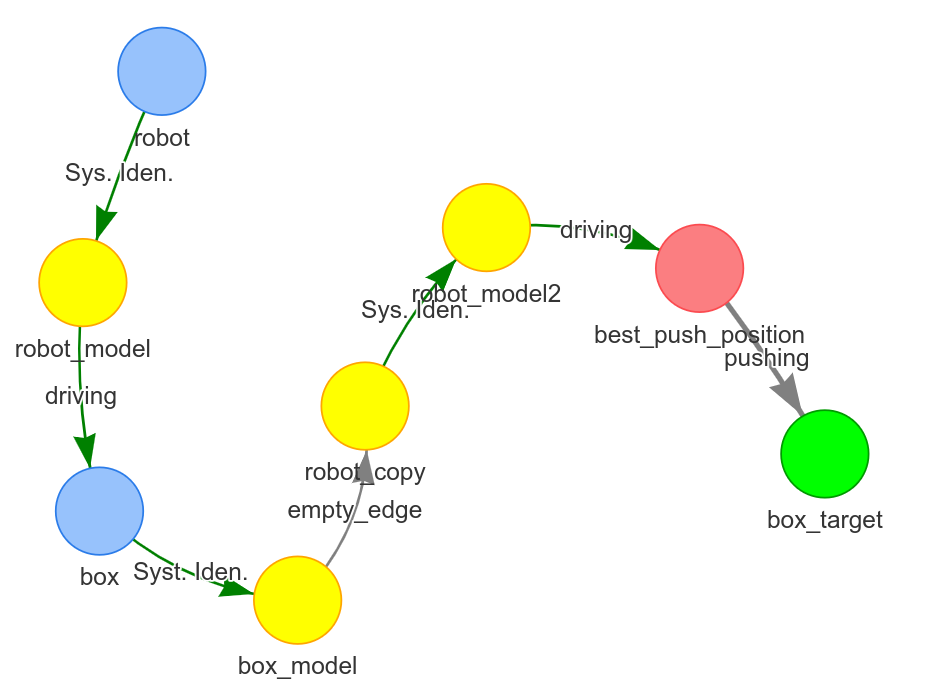
\includegraphics[width=1.05\textwidth]{figures/connecting_nodes/robot_push/robot_push_8}
    \caption{}\label{subfig:robot_push_8}
    \end{subfigure}
    \begin{subfigure}{.3\textwidth}
    \centering
    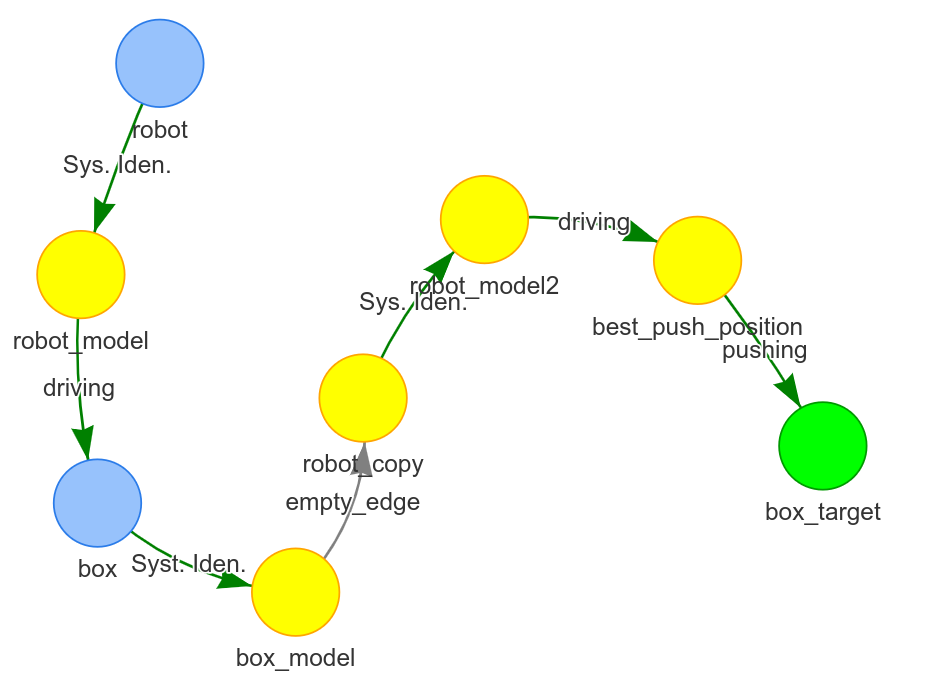
\includegraphics[width=1.05\textwidth]{figures/connecting_nodes/robot_push/robot_push_9}
    \caption{}\label{subfig:robot_push_9}
    \end{subfigure}
    \caption{\ac{hgraph} for pushing the green box to the target configuration}%
    \label{fig:robot_push_hgraph}
\end{figure}
Especially in \cref{subfig:robot_push_2,subfig:robot_push_3} the backward search is clearly visible, the \ac{halgorithm} searches from target node to the robot node. \Cref{fig:robot_push_hgraph} is extensive because every nessecary steps is included whilst some could be skipped. First, identifying a system model for robot driving twice, if the system model created in edge Sys. Iden. pointing toward node robot\_model is reused, then the edge Sys. Iden. pointing toward robot\_model\_1 would be unnecessary. Second, if system models would already be availeble for driving and pushing, no single system identification edge would be required. A \textit{empty\_edge} can be seen in \cref{subfig:robot_push_7,subfig:robot_push_8,subfig:robot_push_9}, the empty\_edge serves to connect a node to another node (box\_model to robot\_copy in \cref{fig:robot_push_hgraph}). The empty\_edge can be traversed without execution, holds no controller, system model or status.\bs

\paragraph{Encountering a Blocked Path}%
During propagation of an action edge's status, motion or manipulation planning occurs. If an object is blocking the path, planning will detect it and the \ac{halgorithm} tries to free the path. In the next example the \ac{halgorithm} detects a blocking object and frees the path by pushing the blocking object to a new configuration, and can be visulised in \cref{fig:blocking_obj_hgraph}.\bs

\begin{figure}[H]
    \centering
    \begin{subfigure}{.3\textwidth}
    \centering
    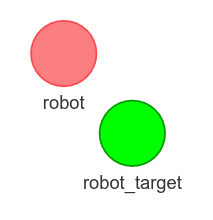
\includegraphics[width=0.5\textwidth]{figures/connecting_nodes/blocking_obj/blocking_obj_1}
    \caption{}
    \end{subfigure}
    \begin{subfigure}{.3\textwidth}
    \centering
    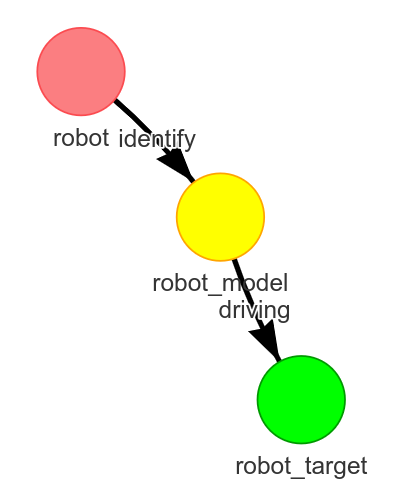
\includegraphics[width=\textwidth]{figures/connecting_nodes/blocking_obj/blocking_obj_2}
    \caption{}\label{subfig:blocking_obj_2}
    \end{subfigure}
    \begin{subfigure}{.3\textwidth}
    \centering
    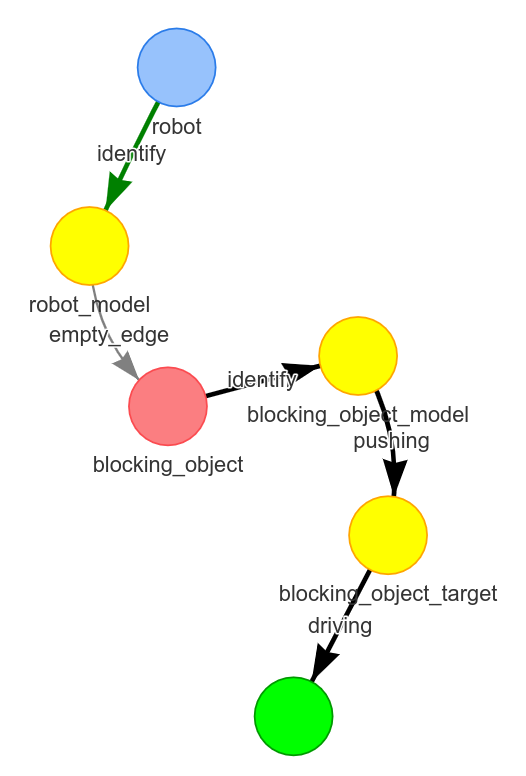
\includegraphics[width=\textwidth]{figures/connecting_nodes/blocking_obj/blocking_obj_3}
    \caption{}\label{subfig:blocking_obj_3}
    \end{subfigure}

    \begin{subfigure}{.3\textwidth}
    \centering
    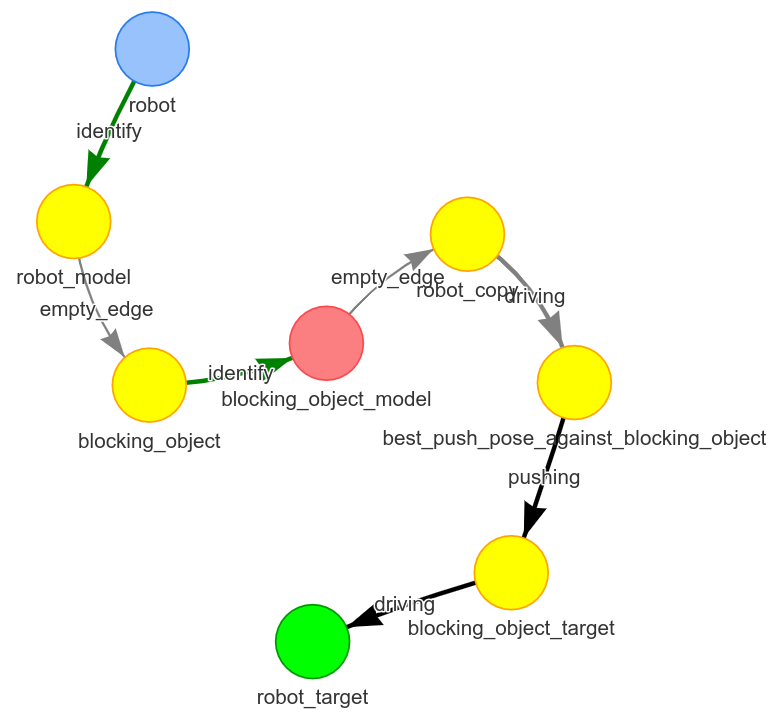
\includegraphics[width=1.3\textwidth]{figures/connecting_nodes/blocking_obj/blocking_obj_4}
    \caption{}\label{subfig:blocking_obj_4}
    \end{subfigure}
    \begin{subfigure}{.3\textwidth}
    \centering
    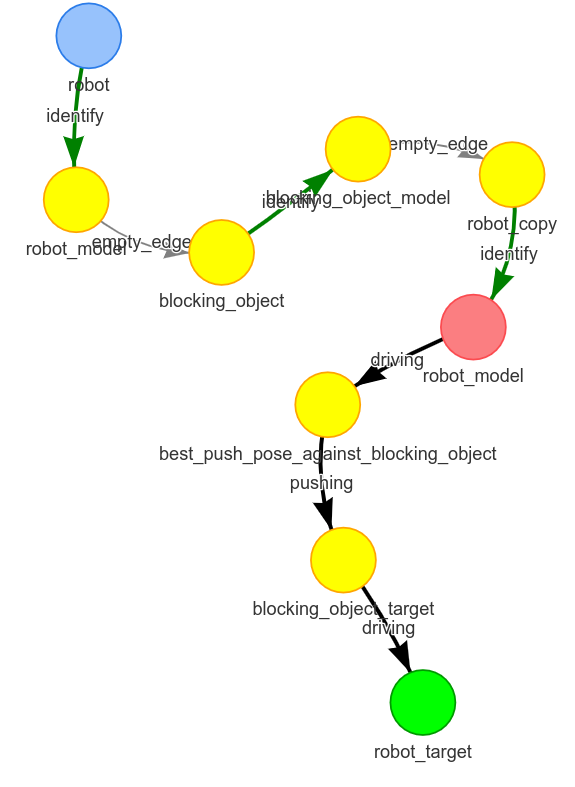
\includegraphics[width=\textwidth]{figures/connecting_nodes/blocking_obj/blocking_obj_5}
    \caption{}\label{subfig:blocking_obj_5}
    \end{subfigure}
    \begin{subfigure}{.3\textwidth}
    \centering
    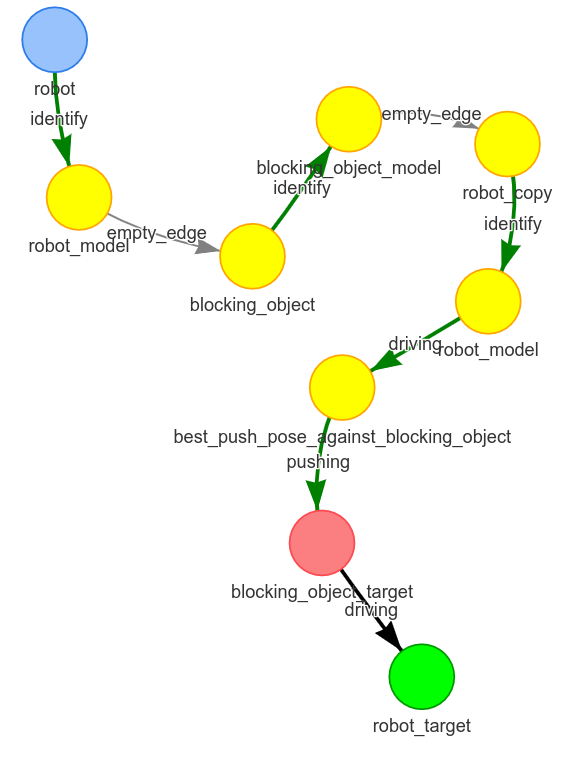
\includegraphics[width=\textwidth]{figures/connecting_nodes/blocking_obj/blocking_obj_6}
    \caption{}\label{subfig:blocking_obj_6}
    \end{subfigure}
    \caption{\ac{hgraph} for driving to target configuration and encountering a blocked path}%
    \label{fig:blocking_obj_hgraph}
\end{figure}

\paragraph{Encountering Failure}%
In the last example, the first hypothesis fails to complete and the \ac{halgorithm} tries to generate a new hypothesis that also fails to complete. Several faults and failures are modelled, the \ac{halgorithm} response to faults and failure is the same. If during the propagation of an edge's status any kind of failure arises, the failed edge and corresponding edges are marked as failed. Equally during execution, if a fault is detected, the execution halts and the edge and corresponding edges are marked as \quotes{failed}, the procedure can be seen in \cref{fig:failure_in_hgraph}.\bs

\begin{figure}[H]
    \centering
    \begin{subfigure}{.3\textwidth}
    \centering
    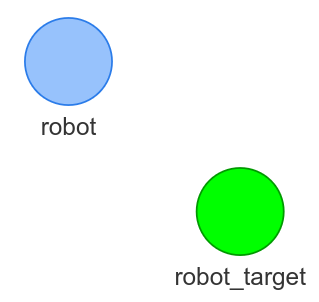
\includegraphics[width=0.8\textwidth]{figures/connecting_nodes/failure/fail_1}
    \end{subfigure}
    \begin{subfigure}{.3\textwidth}
    \centering
    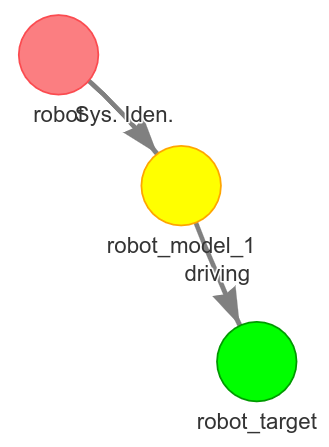
\includegraphics[width=1.1\textwidth]{figures/connecting_nodes/failure/fail_2}
    \end{subfigure}
    \begin{subfigure}{.3\textwidth}
    \centering
    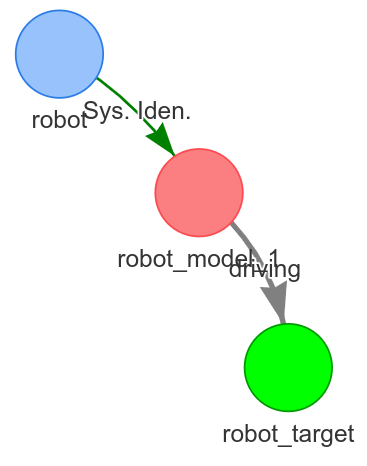
\includegraphics[width=1\textwidth]{figures/connecting_nodes/failure/fail_3}
    \end{subfigure}

    \begin{subfigure}{.3\textwidth}
    \centering
    \includegraphics[width=1\textwidth]{figures/connecting_nodes/failure/fail_4}
    \end{subfigure}
    \begin{subfigure}{.3\textwidth}
    \centering
    \includegraphics[width=1\textwidth]{figures/connecting_nodes/failure/fail_5}
    \end{subfigure}
    \begin{subfigure}{.3\textwidth}
    \centering
    \includegraphics[width=1\textwidth]{figures/connecting_nodes/failure/fail_6}
    \end{subfigure}

    \begin{subfigure}{.3\textwidth}
    \centering
    \includegraphics[width=1\textwidth]{figures/connecting_nodes/failure/fail_7}
    \end{subfigure}
    \hfill
    \caption{Executing two hypothesis, both failing to complete because a fault of failure emerged.}%
    \label{fig:failure_in_hgraph}
\end{figure}

In \cref{fig:failure_in_hgraph} only two parameterisations of drive controller and system model were available. Thus after two failed hypothesis the \ac{halgorithm} concludes it cannot complete this task.\bs


What by now hopefully became clear to the reader is that the \ac{hgraph} autonomously searches for hypotheses to solve the task, one subtask at a time. The \ac{hgraph} switches between the search and execution loop. Switching from the search loop toward the execution loop when a hypothesis is found, and switching back when a hypothesis is completed or an action failed to complete.\bs

The limited number of possible edges (every combination of a system identification method with a compatible control method) guarantees that the robot tries to connect 2 nodes, but concludes that it cannot reach a node if all possible edges have failed. Eventually running out of nodes to connect and conclude that a subtask cannot be completed.\bs

In the next section, the edges that are executed will be reviewed and stored in a knowledge base. The knowledge base will suggest edges when faced with similar nodes to connect.
\

\section{Knowledge Graph}%
\label{sec:kgraph}
The \ac{hgraph} discussed in previous section has a lifetime that spans over a single task, learned system models are not stored for \ac{hgraph} that are created for future tasks. Storing learned environment knowledge is the \ac{kgraph}'s responsibility. Another responsibility of the \ac{kgraph} is to make an ordering in the stored environment knowledge. The ordering is made with a proposed success factor, a metric that combines multiple metrics such as prediction error, tracking error and the success-fail ratio of a edge parameterization (controller and system model). 

\todo[inline]{explainer of the name \ac{kgraph}, Gijs: this is still an open question: Is the name "knowledge graph" correctly chosen? Some comments are that is it misleading because it hints to a knowledge base for which standarts are set. The knowledge graph does not follow these standarts. It is more an ordered list of edge reviews that are bound to a single object.}

\subsection{Definition}
\label{subsec:kgraph_definition}


\todo[inline]{this section}

\subsection{Edge Metrics}
\label{subsec:edge_metrics}
\subsection{Example}
\label{subsec:kgraph_example}



\subsection{Example}%
\label{subsec:kgraph_example}
An example \ac{kgraph} can be visualized in \Cref{fig:kgraph_example}, the parameterization of edges is displayed and the object that the edge controls as image. For clarification, the connected left part with image of the point robot on the center node has 3 outgoing edges that describe robot driving. The connected part on the right with an image of the point robot and the green box on the center node has 2 outgoing edges that describe robot pushing against the green box.\bs

\begin{figure}[H]
    \centering
    \includegraphics[width=10cm]{figures/kgraph_example}
    \caption{\ac{kgraph} with 3 edges on robot driving, and 2 edges for pushing the green box.}%
    \label{fig:kgraph_example}
\end{figure}

The edges in the figure above display only the edge parameterization, but store more information, mainly the success factor. The blue nodes serve a small purpose, making sure edges can point to a node. The blue nodes could fulfill a larger purpose, that is describing which actuators the edge can control. For example, a mobile robot with robot arm attached can have a set of controllers that only drive the base, a set of controllers that only steer the robot arm and a set that controls both the base and robot arm. In such cases the blue nodes describe which part can of the robot can be actuated. The controllers considered in this thesis control every actuator of the robot, resulting in the blue nodes serving such a small purpose.\bs

\subsection{Edge Metrics}%
\label{subsec:edge_metrics}
The \ac{kgraph} keeps an ordered list of `good' and `bad' edge arguments (controller and system model). `Good' and `bad' are defined by edge metrics, these metrics are created after the completion of an edge, regardless of whether the edge was successfully completed or failed. An indication is given on why certain metrics matter in \cref{table:review_edge_metrics}.

\noindent
\begin{table}[H]
\centering
\begin{tabular}%
{>{\raggedright\arraybackslash}p{0.25\textwidth}%
>{\raggedright\arraybackslash}p{0.65\textwidth}}
\acf{PE}&  To better compare prediction errors the \ac{PE} is summarised and average \ac{PE}. The average \ac{PE} is an indicator of an accurate system model but can give misleading results since \ac{PE} is also an indicator of unexpected collisions. Prediction error should thus only be used if there are no collisions detected. The average \ac{PE} comes with more flaws since the average is mostly determined by outliers, some unfortunate outliers in the \ac{PE} might for the largest part determine the average \ac{PE}. The average \ac{PE} will thus not be used because it is not robust enough.\\
\acf{TE}& For a low \ac{TE} the system model must be close to the real motion equations to yield a feasible path, the controller must be well tuned to be able to track that path and the controller and system model must be in collaboration, because the controller uses the system model to calculate system input. A low \ac{TE} tells multiple things, whilst a high \ac{TE} would indicate improvements could be gained in the controller, the system model or their collaboration.\\
ratio num\_succesfully completed edges and num\_total edges & Over time the \ac{kgraph} can recommend the same edge arguements multiple times. Logging the ratio of succeeding edges vs total edges builds an evident portfolio. Still, this metric has to be taken with a grain of salt because edges with equal edge arguments perform similar actions e.g.~pushing an object through a wide corridor is compared to pushing the same object through a narrow corridor. One could say \quotes{comparing apples with pears}.\\
the final position and \newline displacement error & The quality of the result is measured in the final position and displacement error. The importance should thus be stressed when ordering edge arguments.\\
planning time& With system identification, path estimation, motion or manipulation planning the planning time can vary in orders of magnitude between simple or more complex approaches. Planning time mainly serves to rank the slowest planners low, whilst not influencing the rank of fast and average planners.\\
runtime& Also known as execution time would be a quality indicator if start and target states would be equal. Edges are recommended to solve similar tasks, where the path length between the start and target state is different. Thus planning time is not of any use to rank edges.\\
completion time = \newline runtime + planning time & With the same arguementation as runtime, completion time is not of any use to rank edges.\\
\end{tabular}
\caption{Edge metrics used to rank control methods from `good' to `bad'}
\label{table:review_edge_metrics}
\end{table}


\todo[inline]{GIJS: hey, the conclusion for the kgraph is still missing!}



\chapter{Results}%
\label{chap:results}
\textit{This chapter presents the test results that test and challenge the proposed method. Three types of test are introduced which are custom made benchmark tests, randomisation tests and test taken including and excluding the \ac{kgraph}. The test results provide evidence that support the effectiveness of the proposed method. This chapter starts by introducing \textbf{method metrics} that indicate how a task has been executed by the proposed method in \cref{sec:proposed_method_metrics}. Then the three types of test are presented in \cref{sec:benchmark_tests,sec:randomisation,sec:kgraph_on_off}. A comparison is made with the state-of-the-art methods in \cref{sec:compare_with_related_papers}, the chapter is finalised with a discussion about the results in \cref{sec:discussion}.\bs}

\paragraph{The Simulation Environment}
Testing in a simulation environment has been done using the URDF Gym Environment~\cite{spahn_urdfenvironment_2022}, a 100\% python environment build upon the PyBullet library~\cite{coumans_pybullet_2016}. The code created during the thesis can be found on \href{https://gitlab.tudelft.nl/airlab-delft/msc_projects/msc_gijs_groote}{GitLab} and \href{https://github.com/GijsGroote/semantic-thinking-robot}{GitHub}. Experiments ran on standard TU Delft laptop: HP ZBook Studio x360 G5, running OS: Ubuntu 22.04.1 LTS x86\_64, CPU: Intel i7-8750H (12) @ 4.100GHz, GPU: NVIDIA Quadro P1000 Mobile.\bs
The simulation environment provides many different robots, 2 simple robots are selected to perform tests, they are displayed in \cref{fig:example_robots}, and various objects are displayed in \cref{fig:example_objects}.


\todo[inline]{The results will be made in a while, wait for a moment while we try to make sense of the almost-existing results}

\section{Proposed Method Metrics}%
\label{sec:proposed_method_metrics}
The results are measured in method metrics, not to be confused with the monitoring metrics in \cref{sec:monitoring_metrics} or the edge metrics in \cref{subsec:edge_metrics}. The results are interseting, but most interesting is the progression of the method metrics over time. As will be shown, the effect of learning can be measured by investigating tracking the method metrics over time. Furthermore, the method metrics will be used to compare the proposed method to relative state-of-the-art papers. First the method metrics are presented in~\cref{table:proposed_method_metrics} with corresponding argumentation on the relevance of the metric.\bs

\begin{table}[htb!]
\centering
\begin{tabular}[t]{p{4cm} p{10cm}}
Total Average\newline \acl{PE} & The total average \ac{PE} is created by averaging over every hypothesis' average \ac{PE} in a \ac{hgraph}. Since the \ac{PE} is high when unexpected behaviour occurs, seeing the total average \ac{PE} lower would indicate the robot encounters less unexpected behaviour, indicating the robot is learning.\\
Total Average\newline \acl{TE}& The total average \ac{TE} is created by averaging over every hypothesis' average \ac{TE} in a \ac{hgraph}. Seeing the total average \ac{TE} lower over time would indicate the robot is selecting better suitable controllers and system models, indicating the robot is learning.\\
Final positions and\newline displacement errors & The final position and displacement error is a metric which how a controller performs. This thesis does not create or investigate controllers, but it is interesting to see why different controllers are preferred for different objects. The final position and displacement error could be the cause.\\
The ratio between the nubmer of hypothesis and the number of tasks & Expected is that whilst learning system models, the hypothesis created will be more effective. Thus the ratio between the total number of hypotheses and the total number of tasks is expected to lower with new knowledge.\\
The ratio between the number of successfull and the nubmer of total edges in \ac{kgraph} & When the \ac{kgraph} improves recommending a controller and system model, the ratio between successful edges and total edges is expected to increase because, with better recommendations, more edges will be succesfully completed.\\
task completion time =\newline runtime + planning time& If equal tasks are given multiple times, the total task completion time should drop pretty drastically. Multiple factors help to lower the task completion time, firstly system identification has to be performed only once, and there is no need to lose time on redoing system identification. Secondly, the \ac{hgraph} is expected to improve generated hypothesis, or better said, the same mistake should not be made multiple times, resulting in fewer failing hypotheses and lowering task completion time.\\
\end{tabular}
\caption{Proposed method metrics used to compare the proposed method with the state-of-the-art methods.}\label{table:proposed_method_metrics}
\end{table}

\newpage
\section{Benchmark Tests}%
\label{sec:benchmark_tests}
Three benchmark test are now presented, starting with the blockade task. A large part of the proposed method is system identification, for testing however no system identification is performed. Instead a number of hardcoded system models are used, the \ac{kgraph} finds which system model is the best choice for an object over time. Where the best choice is defined using the edge metrics discussed in \cref{subsec:edge_metrics}. Now these hardcoded system models are shortly discussed.\bs

\todo[inline]{define nonlinear-drive-model}
\todo[inline]{define lti-drive-model}
\todo[inline]{define nonlinear-push-model-2}
\todo[inline]{define nonlinear-push-model-2}

\paragraph{Blockade}
\begin{figure}[H]
    \centering
    \includegraphics[width=13cm]{figures/tests/blockade}
    \caption{The blockade environment with the target ghost position for the blue box.}%
    \label{fig:benchmark_blockade}
\end{figure}

The blockade task neatly shows that the \ac{halgorithm} uses the backward search technique. First the \ac{halgorithm} plans to push the box directly to the target position, then it realises a blocking object must first be moved to free the path. It makes the mistake of pushing the unmovable wall, then it succeeds in pushes the movable cylinder out of the way. The \ac{kgraph} then ensures that this mistake will not occur again because is remebered that the wall is immovable. Over time the \ac{kgraph} indicates that it prefers to use the \ac{MPPI} controller with the nonlinear-push-model-2 to push both the box and the cylinder object.\bs
\todo[inline]{is nonlinear-push-model-2 still the preferred model?}

\todo[inline]{results for running the blockade environment multiple times}

\todo[inline]{duck or cylinder, you've told the reader that there would only be boxes and cylinders}
\todo[inline]{tell the reader there also is a duck now, because that duck is really nice I think}

\paragraph{Swap}
\begin{figure}[H]
    \centering
    \includegraphics[width=13cm]{figures/tests/swap}
    \caption{The swap environment, the robot is tasked with swapping the positions of the cylinder and the box.}%
    \label{fig:benchmark_swap}
\end{figure}


\paragraph{Surrounded}
\begin{figure}[H]
    \centering
    \includegraphics[width=13cm]{figures/tests/surrounded}
    \caption{The surround environment, the robot should escape the surrounding enclosure. All box objects are unmovable obstacles with the exception of the green box.}%
    \label{fig:benchmark_surround}
\end{figure}

\section{Randomisation}%
\label{sec:randomisation}
The Randomised environment.\bs
\todo[inline]{write some rand env intro}

\begin{figure}[H]
    \centering
    \begin{subfigure}{\textwidth}
    \centering
    \includegraphics[width=1.0\textwidth]{figures/tests/random_1}
    \end{subfigure}
    \begin{subfigure}{\textwidth}
    \centering
    \includegraphics[width=1.0\textwidth]{figures/tests/random_2}
    \end{subfigure}
    \caption{Two random environment with target ghost configurations for a task that contains 2 subtasks.}%
    \label{fig:random_environnment}
\end{figure}

\begin{figure}[H]
    \centering
    \begin{subfigure}{.49\textwidth}
    \centering
    \includegraphics[width=\textwidth]{figures/tests/random1}
    \end{subfigure}
    \hfill
    \begin{subfigure}{.49\textwidth}
    \centering
    \includegraphics[width=\textwidth]{figures/tests/random2}
    \end{subfigure}

    \vspace{0.2cm}
    \begin{subfigure}{.49\textwidth}
    \includegraphics[width=\textwidth]{figures/tests/random3}
    \end{subfigure}
    \hfill
    \begin{subfigure}{.49\textwidth}
    \centering
    \includegraphics[width=\textwidth]{figures/tests/random4}
    \end{subfigure}
    \caption{A random environments that is reshuffled 4 times. Target ghost configurations are not shown.}
    \label{fig:random_environment_reshuffle}
\end{figure}

% \section{Knowledge Graph On/Off}%
% \label{sec:kgraph_on_off}

\section{Comparison with related papers}%
\label{sec:compare_with_related_papers}

The papers to compare with:\newline

\citefield{sabbaghnovin_model_2021}{title}\\

\cite{sabbaghnovin_model_2021}, 
\todo[inline]{See the paper for tests to reproduce with my hgraph}


\citefield{novin_dynamic_2018}{title}\\
\cite{novin_dynamic_2018}
The following \cite{novin_dynamic_2018} citation is here because it is a refered to from \cite{sabbaghnovin_model_2021} many times




\section{Discussion}%
\label{sec:discussion}

\chapter{Discussion or Conclusions}


Recall the \hyperref[researchquestion:main]{main research question}. \vspace{0.5\baselineskip}\\
\textit{\indent\quotes{How do objects' system models learned by a nonprehensile manipulation robot during task \\ \indent execution improve global task planning?}}\vspace{\baselineskip}

\noindent Before answering the main research question, the two research subquestions are answered.\vspace{\baselineskip}

\noindent Recall \hyperref[researchsubquestion:does_it_work]{first research subquestion}:\vspace{0.5\baselineskip}\\
\textit{\indent\quotes{How does backtracing \cite{krontiris_dealing_2015} while remembering interactions with unknown obstacles compare to\\\indent not remembering learning interactions over time?}}\vspace{0.5\baselineskip}

\noindent The backwards search technique used by the hypothsis graph has shown to succesfully handle uncertain action sequences toward a task completion. Replanning occurs when edges fail to complete. To obtain a clear overview of the effect of learned system model, the effectiveness of the hgraph has been monitored over time in various metrics. Two cases have researched, task execution whilst remebering interaction in the knowledge graph versus task execution without a knowledge graph. The main difference was the time difference because system identification procedure was executed for every edge in the no KGraph case. Another difference was spotted, over time the KGraph case generates hypothesises which completed more often compared to the no KGraph case. \vspace{\baselineskip}


\noindent Recall the \hyperref[researchsubquestion:does_it_compare]{second research subquestion}:\vspace{0.5\baselineskip}\\
\textit{\quotes{Can the proposed method combine learning and planning for push en drive applications? Can the proposed method complete tasks, and how does it compare against the state of the art?}}\vspace{0.5\baselineskip}

The proposed hypothesis graph with assiciated knowledge graph was able to perform as good or better compared to teh state of the art. The proposed method was tested agains existing methods which only a subset of tasks, or 2 of the 3 topics. In comparinson with with\cite{sabbaghnovin_model_2021} the proposed method was shown to perform similar in prediction errors, final displacement error. The proposed method is not designed to optimise a global plan, thus unnessecary driving and pushing can occur. 
\vspace{\baselineskip}

\todo[inline]{anser the main research question}
Now the main question can be answered...


\section{Drawbacks}
\cite{vega-brown_asymptotically_2020} optimises a global path (let's say shortest path to complete a task), the proposed method takes a random subtask which does not even try to converte toward a global optimal path. 

\section{Future work}
\label{sec:future_work}
\todo[inline]{how could the closed-world assumption be removed to resample the real world more?}
\todo[inline]{how could the perfect obstacle sensor assumption be removed to resample the real world more?}
\todo[inline]{how could the task as commutative assumption be removed to resample the real world more?}
\todo[inline]{how could the obstacles do not tip over assumption be removed to resample the real world more?}


\chapter*{Glossary}
\addcontentsline{toc}{chapter}{Glossary}

\subsection*{List of Acronyms}
\vspace{1cm}
\begin{acronym}[]
\acro{MPPI}{Model Predictive Path Integral}
\acro{MPC}{Model Predictive Control}
\acro{NAMO}{Navigation Among Movable Objects}
\acro{NP-hard}{non-deterministic polynomial-time hard}
\acro{NP}{non-deterministic polynomial-time}
\acro{FSM}{Finite State Machine}
\acro{hgraph}{hypothesis graph}
\acro{kgraph}{knowledge graph}
\acro{IO}{Input-Output}
\acro{PE}{Prediction Error}
\acro{TE}{Tracking Error}
\acro{RRT}{Rapidly-exploring Random Tree}
\acro{RRT*}{optimised version of Rapidly-exploring Random Tree}
\acro{LTI}{Linear Time-Invariant}
\acro{LSTM}{Long Short-Term Memory}
\acro{PEM}{Prediction Error Methods}
\acro{IPEM}{Integrated Prediction Error Methods}
\end{acronym}
\vspace{1cm}



%% Prevent urls running into margins in bibliography
\setcounter{biburlnumpenalty}{7000}
\setcounter{biburllcpenalty}{7000}
\setcounter{biburlucpenalty}{7000}

%% Add bibliography
\printbibliography[heading=bibintoc,title=References]

\chapter{Appendix}%
\label{chap:appendix}

\appendix

\textit{This intro to chapter appendix.\bs}

% \section{System Identification Methods}
% \subsection{Prediction Error Minimisation}
% \subsection{Prediction Error Minimisation}
%
% \section{Control Methods}
% \subsection{\acs{MPC}}
% \subsection{\acs{MPPI}}

\chapter{Complexity Classes}%
\label{chap:appendix_complexity_classes}
Problems in class P have a solution which can be found in polynomial time, problems in \ac{NP} are problems for which a solution cannot found in polynomial time. For problems in \ac{NP}, when provided with a solution, verifying that the solution is indeed a valid solution can be done in polynomial time. \ac{NP-hard} problems are a class of problems which are at least as hard as the hardest problems in \ac{NP}. Problems that are \ac{NP-hard} do not have to be elements of NP. They may not even be decidable~\cite{pokharel_computational_2020}. This thesis or other recent studies in the references do not attempt to find an optimal solution. Instead, they provide a solution whilst guaranteeing properties such as near-optimality or probabilistic completeness. We conclude that the \ac{NAMO} problem combined with relocating objects to target positions fall in the category of \ac{NP-hard} problems because it can be reduced to the piano's mover problem.\bs

\chapter{Control Methods}%
\label{chap:appendix_control_methods}

\section{\ac{MPC} Control}
\todo[inline]{Go over this section and update to the standart of the thesis, now that is clearly lit study}
In recent literature involving predictive methods \acf{MPC} methods are dominating, before moving on to \ac{MPC} and variations of \ac{MPC}, \ac{MPC} will briefly be explained.  The basic concept of \ac{MPC} is to use a dynamic model to forecast system behaviour and optimise the forecast to produce the best decision for the control move at the current time. Models are therefore central to every form of \ac{MPC}. Because the optimal control move depends on the initial state of the dynamic system~\cite{rawlings_model_2020}. A dynamical model can be presented in various forms, let's consider a familiar differential equation. 
$$ \frac{dx}{dt} = f(x(t), u(t)) $$
$$ y = h(x(t), u(t)) $$ 
$$ x(t_0) = x_0 $$

In which $x \in \mathbb{R}^n $ is the state, $u \in \mathbb{R}^m$ is the input, $y \in \mathbb{R}^p$ is the output, and $t \in \mathbb{R}$ is time. The initial condition specifies the value of the state $x$ at $t = t_0$, and a solution to the differential equation for time greater than $t_0$, $t \in \mathbb{R}_{\geq 0}$ is sought. If little knowledge about the internal structure of a system is available, it may be convenient to take another approach where the state is suppressed, no internal structure about the system is known and the focus lies only on the manipulable inputs and measurable outputs. As shown in \cref{figure: mpc_block_diagam}, consider the system $G(t)$ to be
the connection between $u$ and $y$. In this viewpoint, various system identification techniques are used, in which $u$ is manipulated and $y$ is measured~\cite{rawlings_model_2020}. From the input-output relation, a system model is estimated or improved. The system model can be seen inside the \ac{MPC} controller block in \cref{figure: mpc_block_diagam}.\\

\begin{figure}[h]
\centering
\begin{tikzpicture}
% blocks
\node[draw,
    minimum width=2cm,
    minimum height=1.2cm,
    fill=myLightColor,
] (system) at (0,0){$G(t)$};
\node[draw,
    minimum width=5.5cm,
    minimum height=2cm,
    fill=myEvenLighterColor,
    below = 1cm of system,
    label=above:MPC controller,
] (controller) {};
% the blocks and arrows inside MPC
\node[draw, minimum width=2cm, below=3mm of controller.north, anchor=north, fill=myDarkColor] (optimisation) {Optimisation};
\node[draw, below=8mm of optimisation.south, anchor=south, fill=myDarkColor] (model) {System Model};
\path[-stealth]
        (model.east) edge[bend right=70] node[pos=0.5, right] {Predict} (optimisation.east)
        (optimisation.west) edge[bend right=70] node[pos=0.5, left] {Action}  (model.west);
% Arrows
\draw[-stealth] (controller.west) |- ($(controller.west) - (1,0mm) $) |- (system.west) 
node[near end, above]{$u(t)$};
\draw[stealth-] ([yshift=-0.3cm]controller.east) -- ++(3,0) node[midway, above](input){$y_{ref}(t)$, $p$, $\mathbb{X}$, $\mathbb{U}$, $\mathbb{Y}$};
\draw[-stealth] (system.east) -- ++ (5, 0) 
    node[midway](output){}node[midway,above]{$y(t)$};
    \draw [-stealth] (output.center) |- ([yshift=0.5cm]controller.east); 
\end{tikzpicture}
\caption{System $G(t)$ with input ${u}(t)$, output $y(t)$ and \acs{MPC} controller with input $y(t)$, reference signal $y_{ref}(t)$, parameterisation $p$ and constraint sets $\mathbb{X}$, $\mathbb{U}$, $\mathbb{Y}$} \label{figure: mpc_block_diagam} \end{figure}  

As indicated in the problem description in TODO, prior knowledge about the structure of the robot itself is known. Such structure can be specified in a parameterisable system model, in which the influence of inputs and current states describes the behaviour of states and outputs. Uncertain parameters have to be sought, such as the center of mass, mass, and diameter of wheels. These parameters reside in the parameterisation $p$, see TODO. \Cref{figure: mpc_block_diagam} shows the parameterisation $p$, for purely analytical system models the parameterisation is left empty. The following explanation about \ac{MPC} is best understood with the differential drive robot in mind from TODO, with single-body model TODO. Some states of the system might be inside an obstacle region, such a region is undesirable for the robot to be in or go toward. The robot states are allowed in free space, which is all space minus the obstacle region. The free space is specified as a state constrained set $\mathbb{X}$. Allowable input can be restricted by the input constraint set $\mathbb{U}$, a scenario in which input constraints are required is for example the maximum torque an engine produces at full throttle. Lastly, the set of allowed outputs is specified in the output constraint set $\mathbb{Y}$. State, input and output constraints must be respected during optimisation, the optimiser takes the state-, input- and output constraint sets $\mathbb{X}$, $\mathbb{U}$, $\mathbb{Y}$ and if feasible, finds an action sequence driving the system toward the reference signal while constraints are respected. The \ac{MPC} system model predicts future states where the system is steered toward as a result of input actions.\\

The optimisation minimises an objective function $V_{N}(x_{0}, y_{ref}, \mathbf{u}_{N}(0))$, where\\ $ \mathbf{u}_{N}(k) = (u_k, u_{k+1}, \dots , u_{k+N})$. The objective function takes the reference signal as an argument together with the initial state and the control input for the control horizon. The objective function then creates a weighted sum of some heuristic function. States and inputs resulting in outputs far from the reference signal are penalised more by the heuristic function than outputs closer to the reference signal. Because the objective function is a Lyapunov function, it has the property that, it has a global minimum for the optimal input $\mathbf{u}_{N}^*$. If the system output reaches the reference signal $y_{ref}$, $x_{ref}$ then $u_{ref}$ will be mapped to the output reference signal as such $y_{ref} = h(x_{ref}, u_{ref})$. As a result solving the minimisation problem displayed in \cref{equation: mpc_problem} gives the optimal input which steers the system toward the output reference signal while at the same time respecting the constraints. 

\begin{mini}
{u_k, u_{k+1}, \dots , u_{k+N}} {
V_{N}(x_{0}, y_{ref}, u_k, u_{k+1}, \dots , u_{k+N})
}
{}{}
\addConstraint{x(k+1) = f(x(k), u(k))}
\addConstraint{x \in \mathbb{X}}
\addConstraint{u \in \mathbb{U}}
\addConstraint{y \in \mathbb{Y}}
\addConstraint{x(0) = x_0}
\label{equation: mpc_problem}
\end{mini}

\Cref{figure: mpc_scheme_basic} displays the predicted output converging toward the constant output reference. After solving the minimisation problem, \cref{equation: mpc_problem}, the optimal input sequence is obtained $\mathbf{u}^*_N$ (given that the constraints are respected for such input), from which only the first input is executed for time step $k$ to $k+1$. Then all indices are shifted such that the previous time step $k+1$ becomes $k$, the output is measured and the reference signal, parameterisation, and constraints sets are updated and a new minimisation problem is created, which completes the cycle. Note that \cref{figure: mpc_block_diagam,figure: mpc_scheme_basic} is an example \ac{MPC} controller, which hardly scratched the surface of \ac{MPC}, there are many variations and additions such as deterministic and stochastic \ac{MPC}, stage and terminal cost, distributed \ac{MPC}, etc. which~\cite{rawlings_model_2020} visits extensively. 

\begin{figure}[h]
    \centering
    \includegraphics[width=0.8\textwidth]{figures/MPC_simple_diagram.png}
    \caption{A discrete \acs{MPC} scheme tracking a constant reference signal. $k$ indicates the discrete time step, $N$ the control horizon}
    \label{figure: mpc_scheme_basic}
\end{figure}

A major flaw for \ac{MPC} was the computation time required to solve a minimisation problem every time step. Because processors' power has increased, the \ac{MPC} framework can be applied in real time and is applicable for robotics. When applied to tracking a reference signal the \ac{MPC} framework outperforms classic control approaches such as PID control~\cite{nascimento_nonholonomic_2018}. Where \ac{MPC} excels at is tracking multiple objectives which can be weighted in the objective function. For example, \ac{MPC} can primarily track a robot path, while secondarily satisfying some additional dynamic specifications. This makes \ac{MPC} especially suitable in path tracking for nonholonomic robots. By restricting the state constraint set, obstacles can be avoided, such obstacles can even be avoided online  because the state constraint set may be changed during execution. It should however be feasible to find an input which satisfies all constraints. Because of its ease of tuning, handling multiple objectives, and flexibility in adding constraints, \ac{MPC} became the baseline standard to compare new control approaches with in control research. By now, linear \ac{MPC} theory is quite mature, and important issues
such as stability are well addressed in the last decade. Nevertheless, some systems are, in general,
inherently nonlinear. Therefore, especially in highly dynamic systems such as mobile robotics, linear
models are often inadequate to describe the process dynamics and nonlinear models have to be used. Thus nonlinear \ac{MPC} theory is required for which closed-loop stability proofs are lacking~\cite{nascimento_nonholonomic_2018}. \\


\section{\ac{MPPI} Control}
\todo[inline]{Go over this section and update to the standart of the thesis, now that is clearly lit study}
Introduced by~\cite{williams_model_2015} \ac{MPPI} control arose. Which was followed by \ac{MPPI} control combined with various system models, identification methods~\cite{abraham_modelbased_2020,cong_selfadapting_2020,arruda_uncertainty_2017}. The core idea is from the current state of the system with the use of a system model and randomly sampled inputs to simulate in the future a number of "rollouts" for a specific time horizon,~\cite{neuromorphictutorial_ltc21_2021}. These rollouts indicate the future states of the system if the randomly sampled inputs would be applied to the system, the future states can be evaluated by a cost function which penalised undesired states and rewards desired future states. A weighted sum over all rollouts determines the input which will be applied to the system. If a goal state is not reached, the control loop starts with the next iteration. An example is provided, see  \cref{figure: mppi_car_with_rollouts}. 

\begin{figure}[h]
    \centering
    \includegraphics[width=0.5\textwidth]{figures/MPPI_car_with_rollouts.png}
    \caption{\acs{MPPI} controlled race car using a control horizon of 3 time steps, with 3 rollouts all having their respected inputs as $u_{i,j}$ where $i$ is the rollout index and $j$ indicates the time step~\cite{neuromorphictutorial_ltc21_2021}.}
    \label{figure: mppi_car_with_rollouts}
\end{figure}

Here 3 rollouts are displayed, The objective function is designed to keep the car driving on the center of the road by penalising rollouts which are further away from the center of the road relatively more. resulting in a high cost for $\text{rollout}_1$ and $\text{rollout}_3$ compared to $\text{rollout}_2$. As a result, the input send to the system as a weighted sum of the rollouts is mostly determined by $\text{rollout}_2$. The weighted sum determining the input is displayed in \cref{equation: mppi_weighted_sum}, from~\cite{neuromorphictutorial_ltc21_2021}.

\begin{equation}
u(k+1)=u(k)+\frac{\sum_{i} w_{i} \delta u_{i}}{\sum_{i} w_{i}}
\label{equation: mppi_weighted_sum}
\end{equation}

Where $\delta u_i$ is the difference between $u(k)$ and the input for rollout $i$, the weight of $\text{rollout}_i$ is detemined as: $w_{i}=e^{-\frac{1}{\lambda} \text{cost}_{i}}$, $\lambda$ is a constant parameter. The reader is now somewhat familiar with the \ac{MPPI} concept, Now some applications with \ac{MPPI} and multi-object control are discussed.\bs

\chapter{Implementation in Python}%
\label{chap:code_implementation}


Code reproducibility in the scientific community is low~\cite{trisovic_largescale_2022}. That is bad, bad bad bad!

\todo[inline]{setup of the system (python version, ubuntu version etc.)}
\todo[inline]{reference to an install readme file}
\todo[inline]{Explain what can be changed easily}
\todo[inline]{Explain code folders (the thingies better to not touch)}
\todo[inline]{Explain code folders (the thingies better to not touch)}
\todo[inline]{What should be done again}

\end{document}
